\documentclass[a4paper, 11pt]{report}

\usepackage{psl-cover}
\usepackage[]{amsmath}
\usepackage[]{physics} % \bra, \ket etc
\usepackage{graphicx} %Pour les figures je crois
\usepackage{hyperref}
\usepackage[
    backend=biber, 
    natbib=true,
    style=numeric-comp,
    sorting=none, %Pour faire apparaitre les refs dans l'ordre
    hyperref=true
]{biblatex} %Imports biblatex package
\addbibresource{bib_thesis.bib} %Import the bibliography file

\usepackage{amssymb} %quelques symboles dont gtrsim /lesssim
\usepackage{subcaption} % package pour faire des subfigures
\usepackage{multirow} % package pour multirow/multicolumn
\usepackage{booktabs} % package pour top/mid/bottom rule
\usepackage{tcolorbox} % toujours plus de boites
\usepackage{xcolor} % Pour avoir des couleurs dans les équations

\title{Cross-relaxation in dense ensembles of NV centers and application to magnetometry \\ \medskip Relaxation croisées d'ensembles de centres NV et application à la magnétométrie}

\author{Clément Pellet-Mary}

\institute{ENS Paris}
\doctoralschool{EDPIF}{564}
\specialty{Physique}
\date{07 Décembre 2022}

\jurymember{1}{Dmitry Budker}{Professor JGU Mainz}{Rapporteur}
\jurymember{2}{Philippe Tamarat}{Professeur, Université de Bordeaux}{Rapporteur}
\jurymember{3}{Maria Chamarro}{Professeure, Sorbonne Université}{Examinateur}
\jurymember{4}{Vincent Jacques}{Directeur de recherche, CNRS}{Examinateur}
\jurymember{5}{Alexandre Tallaire}{Directeur de recherche, CNRS}{Examinateur}
\jurymember{6}{Gabriel Hétet}{Maître de conférences, ENS Paris}{Directeur de thèse}
% \jurymember{9}{Prénom NOM}{Titre, établissement}{Invité}
% \jurymember{10}{Prénom NOM}{Titre, établissement}{Invité}

\frabstract{
Le centre NV du diamant est un candidat prometteur pour de nombreuses technologies quantiques, que ce soit pour les communications quantiques, le calcul quantique ou la métrologie quantique. Grace aux progrès de synthétisation du diamant, des échantillons contenant une haute concentration en centres NV sont aujourd’hui réalisables. Cette augmentation de la densité de centres NV s’accompagne d’une augmentation des interactions entre ces derniers, ce qui donne lieu à une physique complexe et encore largement inexplorée. De nombreuses applications récentes, telles que l’hyper-polarisation en RMN, la bio-imagerie ou encore la spin-mécanique repose sur des ensembles denses de centres NV. Comprendre et maîtriser les propriétés d’ensemble de ces derniers est un point crucial pour l’établissement de ces technologies.

Cette thèse étudie les échanges de polarisation, par relaxation croisée, entre des ensembles denses de centres NV, ainsi que les interactions entre les centres NV et d’autres impuretés paramagnétiques présentes dans le diamant. Le but de ces travaux est de mieux comprendre les propriétés des ensembles de centres NV, et d’exploiter certaines de ces propriétés pour de nouvelles applications telles que la détection d’impuretés ou la magnétométrie.

Dans un premier temps, nous détaillerons les propriétés des centres NV et nous introduirons des concepts liés à l’interaction dipolaire entre spins et aux relaxations croisées. Nous verrons ensuite comment les relaxations croisées peuvent être utilisées pour détecter optiquement des résonances de spins qui ne sont pas optiquement actifs, en l’occurrence les défauts VH- et War1 dans des diamants CVD. Enfin nous étudierons les relaxations croisées entre différents sous-groupes de centre NV. Nous verrons d’abord leur influence sur la dynamique du spin et leur origine microscopique, puis nous étudierons leur dépendance avec le champ magnétique et leur potentielle utilisation pour la magnétométrie en champs faible.
}

\enabstract{
  The NV center in diamond is a promising candidate for emerging quantum technologies, including quantum communication, quantum computing and quantum metrology. Thanks to the recent progress in diamond synthesis, samples with high NV center concentration can now be created. This increase in the NV density comes with an increase of the interaction between them, which leads to a rich and complex physics. Numerous applications, such as NMR hyperpolarization, bio-imagery or spin mechanics rely on the use of dense NV ensembles. Understanding and mastering the properties of ensembles of NV centers will be a crucial point in the development of these technologies. 
  
This doctoral thesis focuses on cross-relaxation between dense ensembles of NV centers, as well as on the interaction between NV centers and other diamond paramagnetic impurities. The aim of this work is to better understand the properties of dense NV centers ensembles, and to exploit them for new applications such as the detection of impurities and magnetometry. 

In the first part, we will detail the properties of single NV centers and introduce notions regarding dipole-dipole spin coupling and cross-relaxations. We will then show how cross-relaxations can be used to optically detect dark spin resonances, in this case the VH- and War1 defects in CVD-grown diamond. Finally, we will present a study of cross-relaxations between subgroups of NV centers. We will first cover the influence of cross-relaxation on the spin dynamics and discuss its microscopic origin. We will then investigate the role of the magnetic field on cross-relaxations as well as their potential use in low field magnetometry.
}

\frkeywords{centre NV, dynamique de spin, magnétométrie}
\enkeywords{NV center, spin dynamics, magnetometry}

\begin{document}

\maketitle{}
\setcounter{tocdepth}{1}

\tableofcontents
 
\chapter*{Introduction}

Quantum mechanics was first developed at the beginning of the 20th century to explain physical observations such as the blackbody radiation \citep{planck1900theorie} or the photoelectric effect \citep{einstein1905erzeugung}. The quantum theory was subsequently developed in the first half of the 20th century and showed great success, in particular in giving a physical framework for chemistry \citep{pauling1931nature} and leading to a microscopic understanding of matter \citep{kittel1996introduction}. In the second half of the 20th century, technological development based on the new understanding of light and matter have led to what was retroactively called the first quantum revolution \citep{thew2019focus}. Technologies developed in the 50s and 60s include the semiconductor transistor \citep{bardeen1948transistor}, the laser \citep{maiman1960stimulated}, and nuclear magnetic resonance \citep{abragam1961principles} which have since revolutionized the fields of information science, global communications and medical imaging. 

A new field of quantum technology has emerged in the last two decades. This ``second quantum revolution" differs from the first one in the usage of individual quantum systems, such as single photons \citep{gleyzes2007quantum}, atoms \citep{neuhauser1980localized} or electrons \citep{peil1999observing}, which have properties that can not be emulated by larger classical systems. These properties include quantum entanglement, superposition or measurement and form the basis of the newly formed quantum information science \citep{nielsen2002quantum, vedral2006introduction, hayashi2006quantum}. 

Central to quantum information science is the idea of quantum bits or qubits \citep{schumacher1996sending}, which are the building blocks of quantum information in analogy to the bits of classical information theory. Physical implementation of a qubit could be any quantum system with two well defined quantum states, as long as these states can be initialized, manipulated and readout \citep{divincenzo2000physical}. Popular qubit candidates include superconducting circuits \citep{nakamura1999coherent, orlando1999superconducting}, photons \citep{bennett1992quantum, zhong2020quantum}, quantum dots \citep{veldhorst2014addressable, zajac2018resonantly}, trapped ions \citep{friis2018observation, wright2019benchmarking} and single crystal defects \citep{jelezko2006single, baranov2011silicon, zhong2015optically}.

Defects in large band gap crystals are sometimes referred to as artificial atoms \citep{buluta2011natural}, as the localized wave function of the electrons surrounding the impurity  give rise to discrete energy levels similar to that of an atom. Of all the possible crystals and defects, the most studied defect for quantum applications is the negatively charged nitrogen-vacancy center in diamond \citep{aharonovich2016solid, de2021materials}, often abbreviated to ``NV center". Although this defect had been known and correctly identified almost 50 years ago \citep{davies1976optical}, interest in the NV center really sparked after it was first isolated in 1997 \citep{gruber1997scanning}. The detection of single NV centers proved that NV centers fluoresce brightly \citep{gruber1997scanning}, are photostable \citep{kurtsiefer2000stable}, and that their electronic spin can be polarized and readout optically \citep{jelezko2004observation}, making them an promising solid state qubit.

Since then, single NV centers have been successfully used to create quantum entanglement over several km \citep{hensen2015loophole}, to store quantum information at room temperature for more than one second \citep{maurer2012room}, to detect single proteins via nuclear magnetic resonance \citep{lovchinsky2016nuclear}, and for many other applications in quantum communication \citep{wehner2018quantum}, quantum computing \citep{de2021materials} or quantum sensing \citep{degen2017quantum}.

As the interest in single NV center grew, diamond synthesis improved significantly \citep{achard2020chemical, barry2020sensitivity, edmonds2020generation}  which benefited not only single NV centers but also NV center ensemble. While single NV center are required for most quantum information processes \citep{ladd2010quantum}, several other applications benefit from a greater concentration of defects and are therefore more suited to operate with NV centers ensemble. Four of these applications are pictured in Fig. \ref{shema introduction}.

\begin{figure}[h!]
\centering
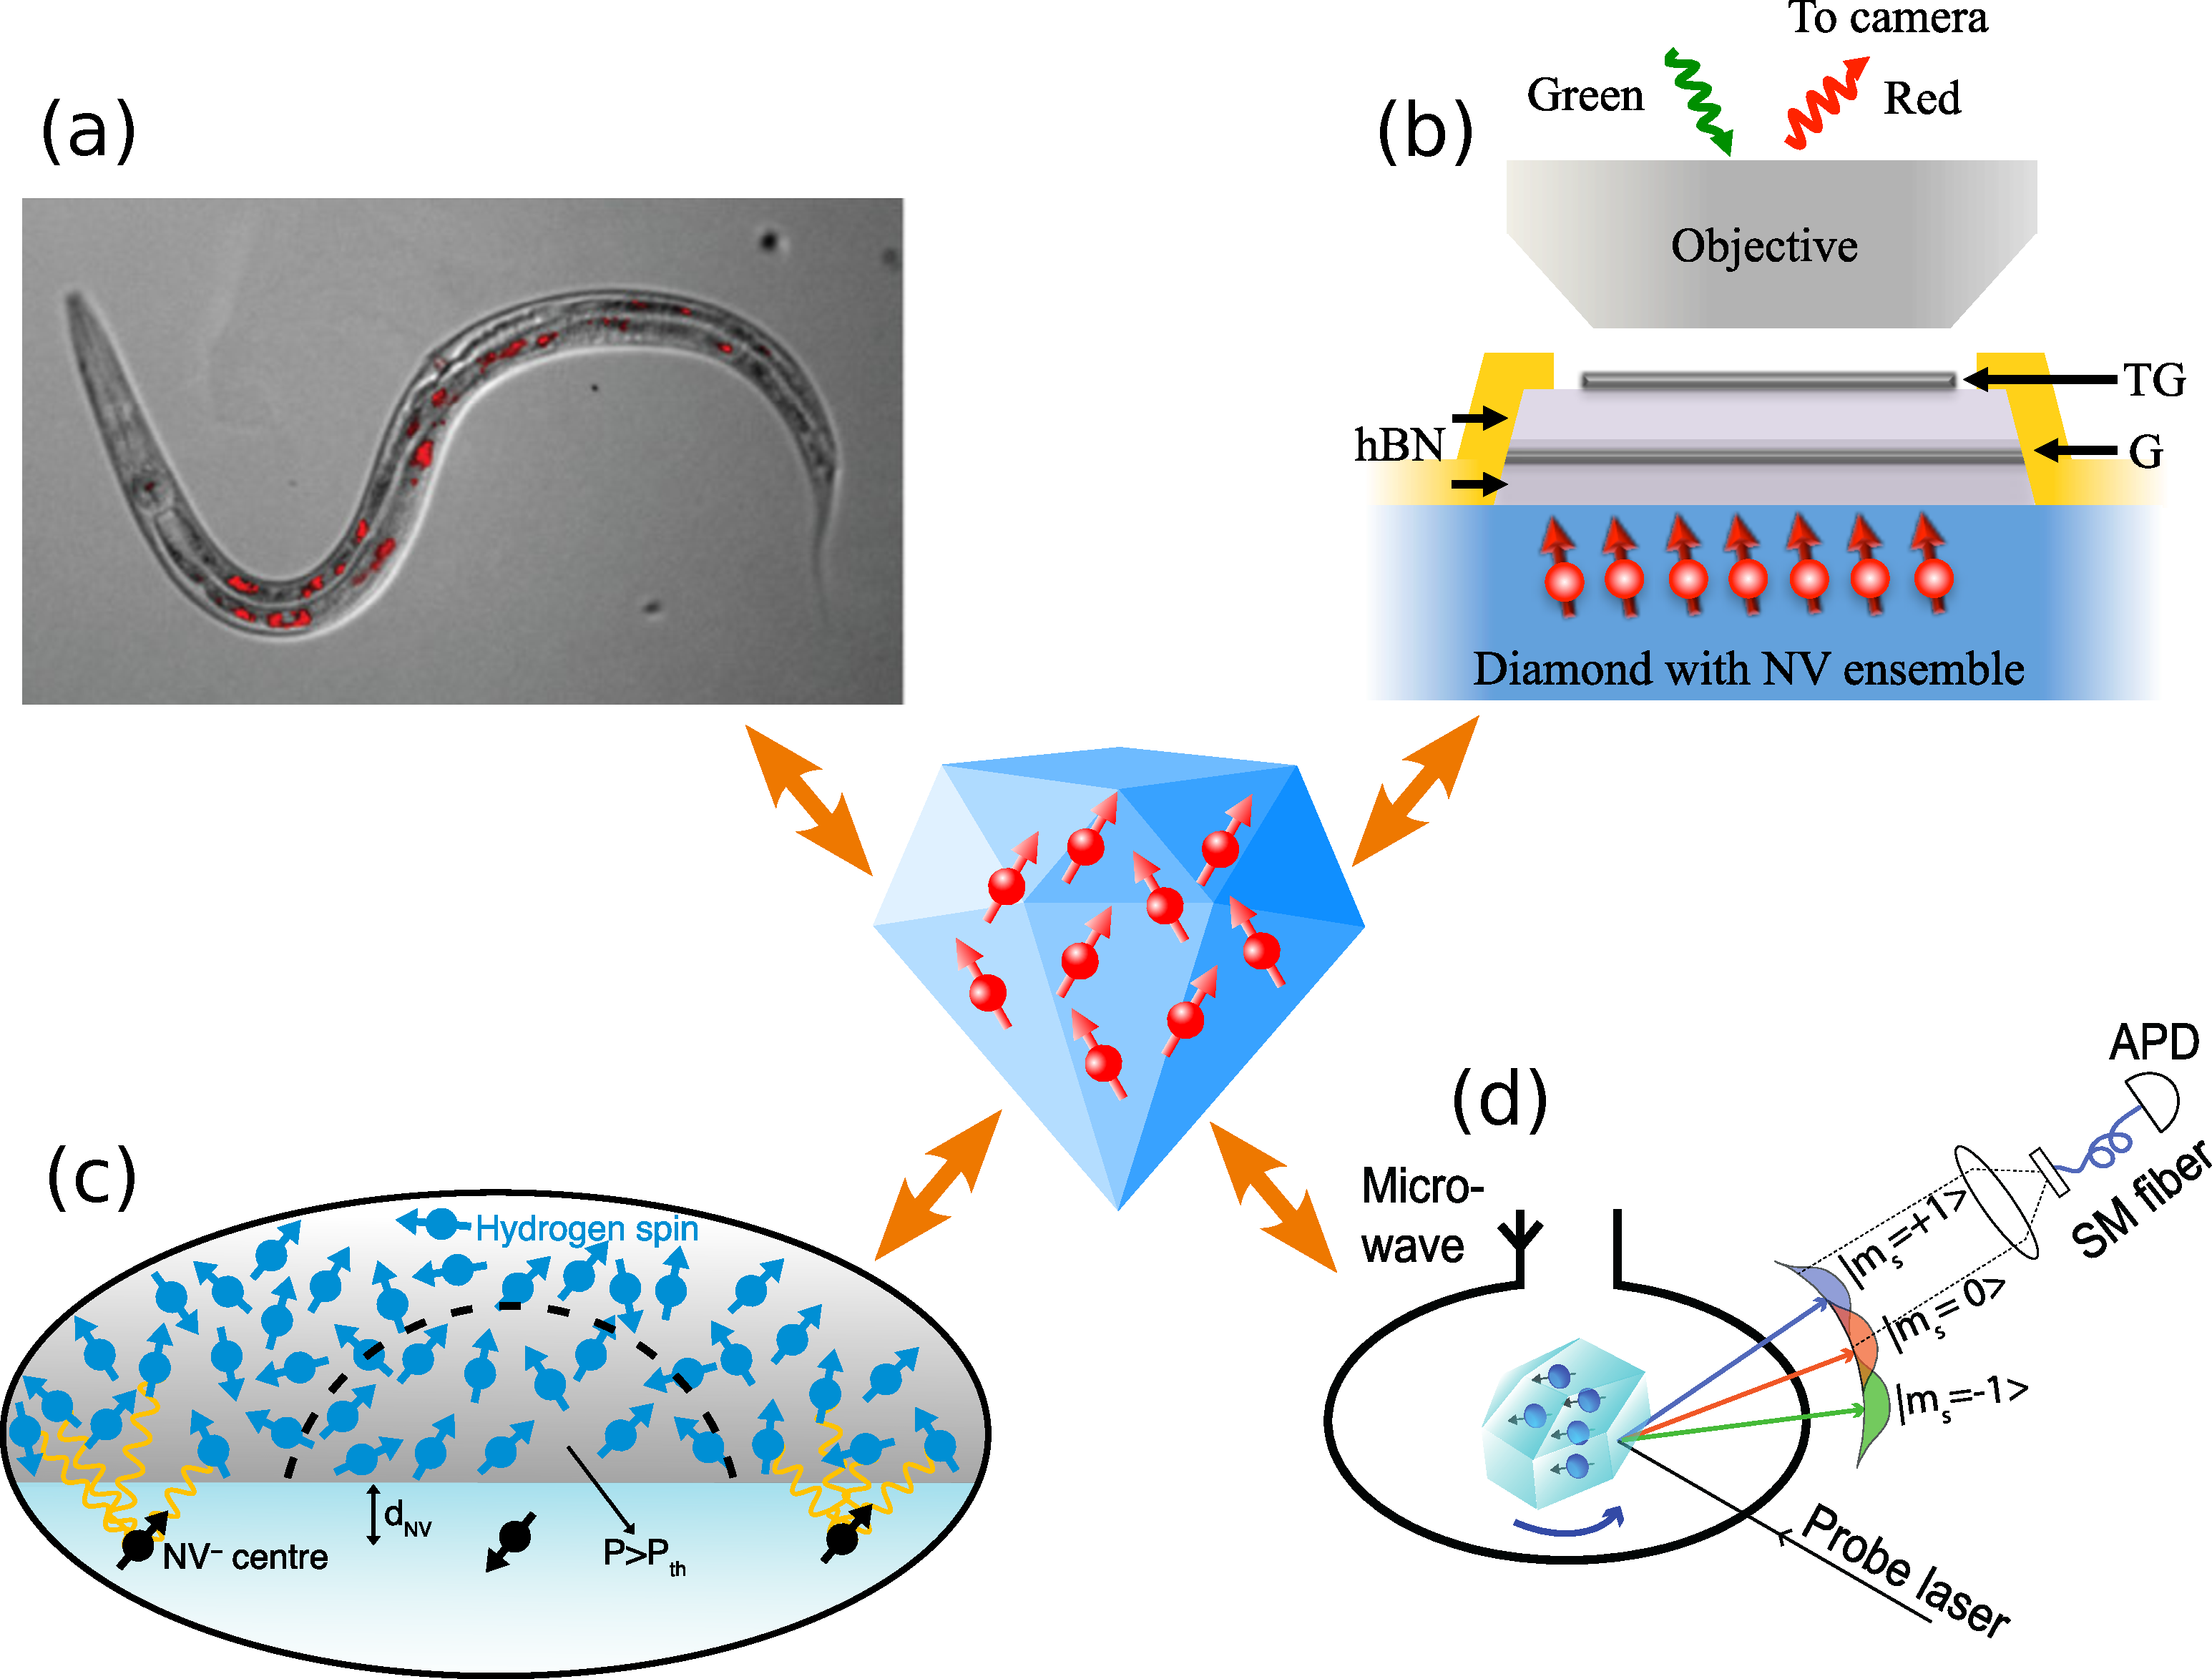
\includegraphics[width=.9\textwidth]{Intro et conclusion/Figures/Fig_intro}
\caption{Example of applications with dense ensemble of NV centers. (a) In vivo nanodiomond biomarkers (from \citep{mohan2010vivo}). (b) Quantum sensing with NV ensemble (from \citep{ku2020imaging}). (c) Dynamic nuclear polarization of an external spin bath (from \citep{healey2021polarization}). (d) Spin mechanics with trapped micro diamonds (from \citep{delord2020spin}).}
\label{shema introduction}
\end{figure}

The first application for NV center ensemble is the use of nano or micro diamonds as fluorescent biomarkers \citep{fu2007characterization, mohan2010vivo}. NV centers are good candidates for biomarkers as they emit a bright and stable photoluminesecence, and because diamond nanocrystals present low toxicity \citep{schirhagl2014nitrogen}. Some applications also use the spin degree of freedom of the NV centers, either to perform background free fluorescence microscopy \citep{chapman2013background} or to monitor the angular motion of the nanodiamonds \citep{mcguinness2011quantum, feng2021association}. For most of these applications, NV ensemble provide a better visibility than single NV centers and are therefore preferred.

The second NV ensemble application is for quantum sensing \citep{degen2017quantum}. NV centers are predominantly used as magnetic field sensors \citep{rondin2014magnetometry, barry2020sensitivity}, although they can also detect electric fields \citep{dolde2011electric, michl2019robust}, temperature \citep{acosta2010temperature, kucsko2013nanometre} ,crystal strain \citep{ovartchaiyapong2014dynamic, doherty2014electronic} or rotation \citep{ledbetter2012gyroscopes, ajoy2012stable}. Both single and ensemble of NV centers can be used for sensing: single centers offer unmatched spatial resolution \citep{mitchell2020colloquium} down to a few nm \citep{lovchinsky2016nuclear}, while ensemble provide better sensitivities \citep{wolf2015subpicotesla, barry2020sensitivity}. 

The third NV ensemble application is nuclear magnetic resonance (NMR) dynamical nuclear polarization \citep{eills2022spin}. Dynamic nuclear polarization consists in increasing the nuclear polarization of a sample by transferring electron polarization to the nuclei bath \citep{abragam1978principles}. Because the NV electronic spin can be optically polarized at room temperature, micro and nano diamonds containing NV centers are promising candidates as hyperpolarization agents \citep{tetienne2021prospects}. Nuclear polarization of spins inside the diamond lattice was demonstrated with single NV centers \citep{jacques2009dynamic, smeltzer2009robust} and NV ensemble \citep{king2015room, scheuer2016optically, schwartz2018robust}. Polarization transfer to nuclear spins outside of the diamond is an ongoing challenge \citep{eills2022spin, healey2021polarization}, but dense NV ensemble are believed to be necessary to achieve high external polarization \citep{tetienne2021prospects, rizzato2022polarization}.

Finally, the fourth NV ensemble application is the recent field of spin mechanics \citep{perdriat2021spin}. Similarly to optomechanics \citep{aspelmeyer2014cavity}, the goal of spin mechanics is to couple a quantum system to the mechanical degree of freedom of a macroscopic object. Strong coupling between single NV center and an external mechanical oscillators has been observed \citep{rabl2009strong, kolkowitz2012coherent}, but coupling between NV centers and the motion of the diamond has so far only been achieved with dense NV ensemble \citep{delord2020spin, pellet2021magnetic, perdriat2022angle}. Coupling several NV centers to the same mechanical oscillator could also lead to interesting magnetic phase transitions \citep{wei2015magnetic, ma2017proposal}.
   
Most of the NV ensemble experiments discussed previously work under the assumption that the ensemble is constituted of $N$ independent single NV centers. However, as often in physics, \textit{more is different} \citep{anderson1972more}. Interaction between the NV center themselves or with their environment can lead to significantly different behavior between ensemble and single spins. These difference include a modification of the charge state dynamics \citep{giri2018coupled} and of the spin dynamics \citep{dobrovitski2008decoherence, jarmola2012temperature, mrozek2015longitudinal, choi2017depolarization}, as well as the apparition of exotic phenomena such as time crystal phase \citep{choi2017observation}, Anderson localization \citep{kucsko2018critical} or superradiance \citep{bradac2017room, angerer2018superradiant}. 

The work presented in this manuscript focuses on dipolarly coupled dense ensemble of NV centers. More specifically, we look at spin polarization exchange between the NV centers themselves and with their environment. Polarization exchange (flip-flop, spin diffusion, cross-relaxation, ...) in dense ensemble of spins has been abundantly studied in the context of NMR \citep{abragam1978principles} and spintronics \citep{vzutic2004spintronics}. Because NV centers tend to be relatively dilute, the question of spin exchange between between NV themselves \citep{choi2017depolarization} or with their environment \citep{hall2016detection} has only recently been addressed. However, as samples with higher NV concentration become available \citep{acosta2009diamonds, tallaire2020high, shenderova2019synthesis}, these aspects are becoming more and more relevant.

The goal of this present work is both to better understand the physics of dense NV ensemble, which is crucial for many of the NV ensemble applications cited previously, and to exploit some of these many-body properties for new applications.

\bigskip
This manuscript is organized in the following way:

\medskip
The first chapter introduces the theoretical and experimental concepts used in this manuscript. This includes a brief overview of diamond and NV centers fabrication processes, the physics of single NV centers and a presentation of magnetic dipole-dipole interaction and cross-relaxation.

The second chapter covers the observation of cross-relaxation between NV centers and other spin impurities in CVD-grown diamond. We use measurements on the NV centers to identify these impurities and to quantify some of their attributes. Most of the results of this chapter have been published in  \citep{pellet2021optical} and \citep{ngambou2022improving}.

The third chapter focuses on the dipole-dipole mediated spin relaxation within dense ensemble of NV centers. Following the work presented in \citep{choi2017depolarization}, we introduce the concept of NV-flutcuator to explain this phenomenon and present experimental and theoretical results solidifying this hypothesis. The results of this chapter have been partly published in \citep{pellet2022spin} and \citep{pellet2021magnetic}.

Finally, the fourth chapter presents a study on NV-NV dipolar relaxation under low magnetic field. This chapter covers both the rich physics of NV centers under low magnetic field, and a potential application of the low field depolarization as a new magnetometry protocol, as well as comparisons with other NV magnetometry protocols. The results of this chapter have in large part been published in \citep{pellet2022spin}.


\chapter{Spin properties of single and ensemble NV centers}
The aim of this first chapter is to introduce concepts related to Nitrogen-vacancy (NV) centers, to the diamond material, and to the dipole-dipole interaction which are necessary to explain the work presented in the later chapters.

In this introductory chapter, we will first cover the material aspects of NV centers by focusing on the creation process of synthetic diamonds and the required steps to create NV defects inside them. We will then cover the optical and spin properties of single NV centers, and introduce the notions of dipole-dipole interaction and cross-relaxation. We will then cover basic experiments with NV centers and introduce the experimental tools required to characterize the NV center's spin. 

\section{The NV center as a physical object}
\begin{figure}[h!]
\centering
\includegraphics[width=0.9\textwidth]{chapter 1/Figures/diamant_et_NV}
\caption{From the diamond to the NV center. a) Drawing of a ``bulk" (macroscopic) diamond. b) Drawing representing a fluorescence microscopy image of a diamond surface. The red fluorescent spots symbolize NV centers photoluminescence. c) Zoom on the crystalline structure of an NV center. Black balls represent carbon atoms}
\label{diamond+NV}
\end{figure}
Before studying the NV centers properties, we must first discuss the diamond itself and answer these questions: How are diamond created, what kind of defects are there in diamond, and how to specifically create NV defects. The field of material science related to diamonds and NV centers is a rich and complex one, and this section will only touch upon basic notions regarding these subjects.

Fig. \ref{diamond+NV} illustrates the various scales to consider in the study of NV centers. Starting with a bulk diamond, typically few mm wide, then zooming-in on the diamond surface with an optical microscope to find fluorescent spots corresponding to the photoluminescence of NV centers. Standard confocal microscopy is limited in its resolution to the $\sim \mu$m range, but if it was possible to zoom-in even further, we would see the atomic structure of a few \AA \ illustrated in the last panel. 
\subsection{Diamond material overview}
\begin{figure}[h!]
\centering
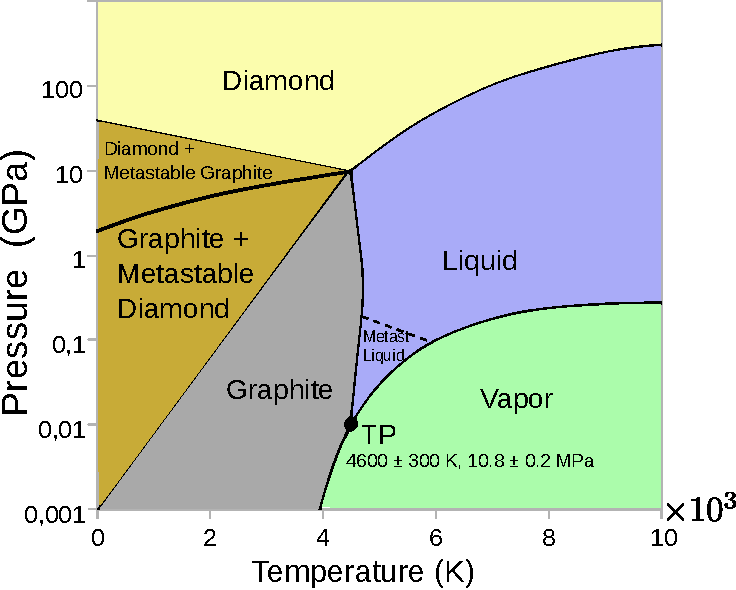
\includegraphics[width=0.6\textwidth]{chapter 1/Figures/phase_diagram_carbon_wiki}
\caption{Pressure-temperature phase diagram of elemental carbon. Credits: Wikimedia commons, adapted from \citep{bundy1989pressure, bundy1996pressure}.}
\label{carbon phase diagram}
\end{figure}

Diamond is a remarkable material in many respects. It is famous for being the hardest and most thermally conductive non-synthetic material. It is also a material with high optical refractive index and optical dispersion which makes it an extremely valuable crystal in jewelry.

Diamond is also famous for being extremely rare in nature, even though its only constituent, carbon, is one of the most abundant element on the Earth surface. The reason being that graphite, and not diamond, is the thermodynamically stable phase of carbon under ambient conditions.

Fig. \ref{carbon phase diagram} shows the PT phase diagram of elemental carbon. We can see that diamond becomes the thermodynamically stable phase only for pressure above a few GPa, $10^4$ times higher than atmospheric pressure. Even though diamond is unstable under ambient conditions, the extremely high energy activation needed to break the sp$^3$ bond between two carbon atoms means that the kinematics of the $C_{\rm diamond} \to C_{\rm graphite}$ transition is almost completely frozen. In many ways diamonds are more stable than graphite under ambient condition due to their relative chemical inertness.

Where the thermodynamic equilibrium really matters is for the crystallization process. The higher pressure needed to reach the diamond-stable region can only be found naturally deep under the earth crust, typically between 150 and 240 km below sea level \citep{tappert2011diamonds}, which explain their scarcity. It also explains why, despite many previous attempts, diamonds were only synthetically produced in 1953 \citep{barnard2000diamond}, more than 50 years after the first synthetic sapphires. To this day, artificial diamond synthesis remains an active field of research \citep{shenderova2019synthesis, achard2020chemical}.

Diamonds grown naturally or artificially are used in the lab and in industry for their extreme hardness, with applications ranging from abrasive to diamond anvil cells \citep{jayaraman1983diamond}. More recently, diamonds have been the object of optics and electronics applications. For both of these fields however, the focus is no longer solely on the diamond but also on the defects hosted inside it.

\subsection{Point defects in diamond}
\begin{figure}[h!]
\centering
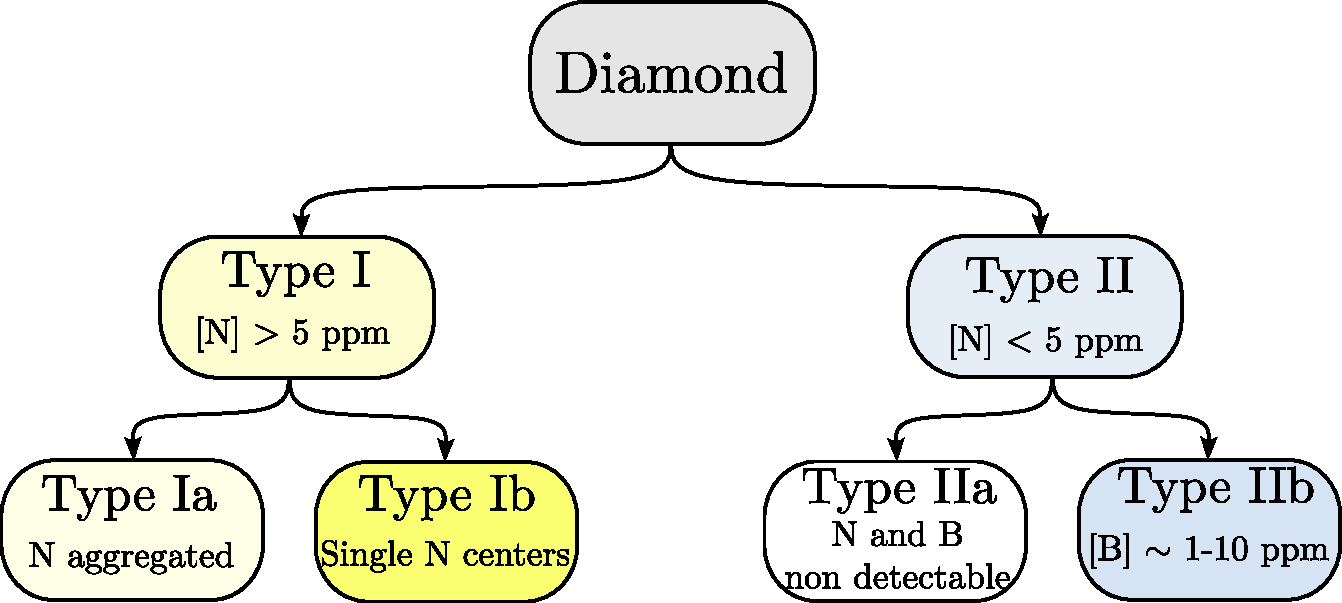
\includegraphics[width=0.9\textwidth]{chapter 1/Figures/Diamond_type}
\caption{Traditional classification of diamonds, based on \citep{tappert2011diamonds}.}
\label{diamond type}
\end{figure}
Diamond in its intrinsic form is an insulator with a bandgap of $\sim 5.47\ \rm eV$ and is transparent from far infrared to deep UV. As any crystal however, diamond is prone to defects. We will focus here on point-like (0D) defects and omit structural defects such as dislocations, even though those too can affect the optical properties of the diamond \citep{collins2000colour}. 

Point-like defects can be constituted by the absence of a carbon atom (``vacancies"), an interstitial defect between two carbon atoms or the substitution of a carbon atom with another atom. These impurities result in unpaired electron or holes localized around the impurity site. This localization causes discrete energy levels for the holes or the electrons, some of which lie inside the diamond bandgap and impact the crystal optical and electrical properties. 

Defects with electronic transitions in the optical range are called ``colored centers" as they are responsible for the coloring of the gems.  Over 20 elements are known to form colored centers when introduced in diamond \citep{zaitsev2013optical, shenderova2019synthesis}, and each of these elemental atoms can form several defects. Nitrogen alone can form more than 50 different colored centers \citep{dobrinets2016hpht, ashfold2020nitrogen}.

Nitrogen, and to a lesser extant boron, are the most commonly found extrinsic elements in natural diamond. The traditional classification of diamond is presented in Fig. \ref{diamond type}. It is based on the N and B concentration, with a threshold of a few ppm (part per million) for each species as this was the smaller amount easily detectable through IR absorption. Type Ia diamonds contain clustered N defects such as the B-center (N$_4$V defect). In contrast, type Ib diamond mostly contains C-center which are single substitutional N$_s$ defects, also referred to as P1 centers in the spin community. Type IIb diamond contains boron impurities which give them a blueish-grey color, and type IIa diamond contains no detectable impurities via IR absorption \citep{ashfold2020nitrogen}.

Nitrogen-vacancy centers are a rare occurrence in both natural diamonds and untreated synthetic diamonds, but we will see later that the much more common N$_s$ defects can be converted in NV centers. When working with NV centers, the starting crystal is therefore often a type Ib diamond if one wants to work with ensemble, or a type IIa diamond if one wants to work with single NV centers \footnote{In order to isolate single NV in a confocal optical spot, the concentration needs to be [NV] $<$ 1 ppb.}.

The boron defects are mainly studied in the context of p-doped diamond semi-conductor: a concentration of [B] $\approx 1000\ \rm ppm$ is needed to achieve a significant overlap between the impurity sites, which turns the diamond into a semi-metal \citep{macpherson2015practical}. Other defects of interest, generally not present naturally but introduced voluntarily, include P and S defects to create n-doped diamond \citep{das2022diamond} (still an active field of research), as well as group IV-vacancy defects (SiV, GeV, SnV, PbV) for quantum optics application \citep{bradac2019quantum}. 

The NV center however remains by far the most studied defect in diamond due to its unique spin properties which will be detailed below.

\subsection{Creation of synthetic diamond for optics and electronics applications}
\begin{figure}[h!]
\centering
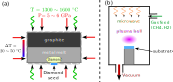
\includegraphics[width=\textwidth]{chapter 1/Figures/HPHT_and_CVD}
\caption{Schematics of HPHT (a) and CVD (b) growth process as detailed in main text}
\label{HPHT and CVD}
\end{figure}

Almost all diamonds used in optics or electronics experiments today are synthetic, due to the higher control of the growth process required for these applications. There are two main competing technologies for the growth of large ($\mu \rm{m} \sim \rm{mm}$) single crystal diamonds: High pressure high temperature growth (HPHT) and chemical vapor deposition growth (CVD). Both of these processes have their own specificities which are detailed below.

\subsubsection{HPHT growth}

HPHT was the first commercially viable process for synthetic diamonds, starting from the 1950s \citep{barnard2000diamond, bundy1955man}. The basic idea of HPHT synthesis is to reconstruct an environment where diamond is the thermodynamically stable phase of carbon, similarly to the growth process of natural diamond below the earth surface. 

Fig. \ref{HPHT and CVD}-a) illustrates the apparatus of HPHT synthesis: a carbon source (graphite) and a solvent metal composed of transition metals (Fe, NI, Co typically \citep{bundy1963direct}) are put under $5 \sim 6$ GPa pressure in a press and heated to temperatures $\geq 1300\ ^\circ$C. A diamond crystal seed is put in the metal melt and a temperature gradient insures that the carbon migrates from the graphite to the diamond.

The first synthesis of HPHT diamonds were all of type Ib due to unwanted nitrogen pollution in the metal melt. The first HPHT type IIa diamonds were produced in the late 90s by adding other elements to the metal bath (Ti, Al, Zr) which would react preferentially with nitrogen and prevent its incorporation in the diamond \citep{burns1999growth, sumiya2002growth}.

\subsubsection{CVD growth}
\label{fab HPHT}

Diamond growth by CVD also started in the 50s, but only really took off in the 80s \citep{matsumoto1982growth, matsumoto1982vapor, kamo1983diamond} with the introduction of atomic hydrogen catalysis. Unlike HPHT, CVD operates in a regime where diamond is not the thermodynamically stable phase. It relies therefore heavily on catalysts to stabilize the diamond phase versus the graphite one. 

The main catalyst used is atomic hydrogen because it etches the $C-C$ sp$^2$ bonds (graphite) faster than it does sp$^3$ bonds (diamond) \citep{gracio2010diamond}. In modern CVD growth, hydrogen is by far the most abundant element in the gas phase: the precursor gases used for the growth are typically CH$_4$ and H$_2$ in proportions of $1-5\%$ and $95-99\%$ respectively \citep{achard2020chemical}.

Fig. \ref{HPHT and CVD}-b) illustrates the apparatus of a microwave plasma reactor: it consists in a modified vacuum chamber which acts as a microwave resonator. The microwave creates a plasma ball from the the precursor gases with a temperature $T_{\rm plasma} \geq 3000 ^\circ$C \citep{ashfold2020nitrogen}, enough to dissociate the $H_2$ gas in atomic hydrogen \citep{balmer2009chemical}. The plasma acts as the carbon source for the diamond growing on top of the substrate, and as the catalyst to favor the diamond phase. %The substrate is kept at a temperature $700 \sim 1100\ ^\circ$C during the growth.

Other sources can be used to create the high temperature required for atomic hydrogen, such as a tungsten hot filament \citep{haubner1993diamond}, electrical discharge (arcjet) \citep{luque1998excited} or even an oxygen-acetylene combustion flame \citep{bachmann1991towards}.

If the CVD reactor is well built, the main sources of extrinsic impurities in the diamond comes from the source gasses \citep{balmer2009chemical}. The commercial availability of source gases containing less than $\sim$ ppm impurities made possible the growth of  high purity type IIa CVD diamonds \citep{kasu2003high, twitchen2004high, tallaire2006characterisation}.

\medskip
Both HPHT and CVD processes can produce diamonds of high quality for quantum optics or electronics application, each with their own pros and cons. HPHT offers better scalability for thick crystals ($\sim \rm mm$) and allows the incorporation of heavy atoms (Ge \citep{palyanov2015germanium} , Sn \citep{ekimov2019effect}) which can be hard to incorporate from a gas phase. CVD on the other hand allows more versatility in the control of the impurities introduced in the crystal, including an isotopic control on both the impurities and the carbon itself. A particular advantage of CVD growth is the possibility of $\delta$-doping where a specific defect is grown only within a thin layer of the crystal, as low as 5 nm \citep{ohno2012engineering, ishikawa2012optical, ohashi2013negatively}.

\subsection{Optimizing NV center formation}
\begin{figure}[h!]
\centering
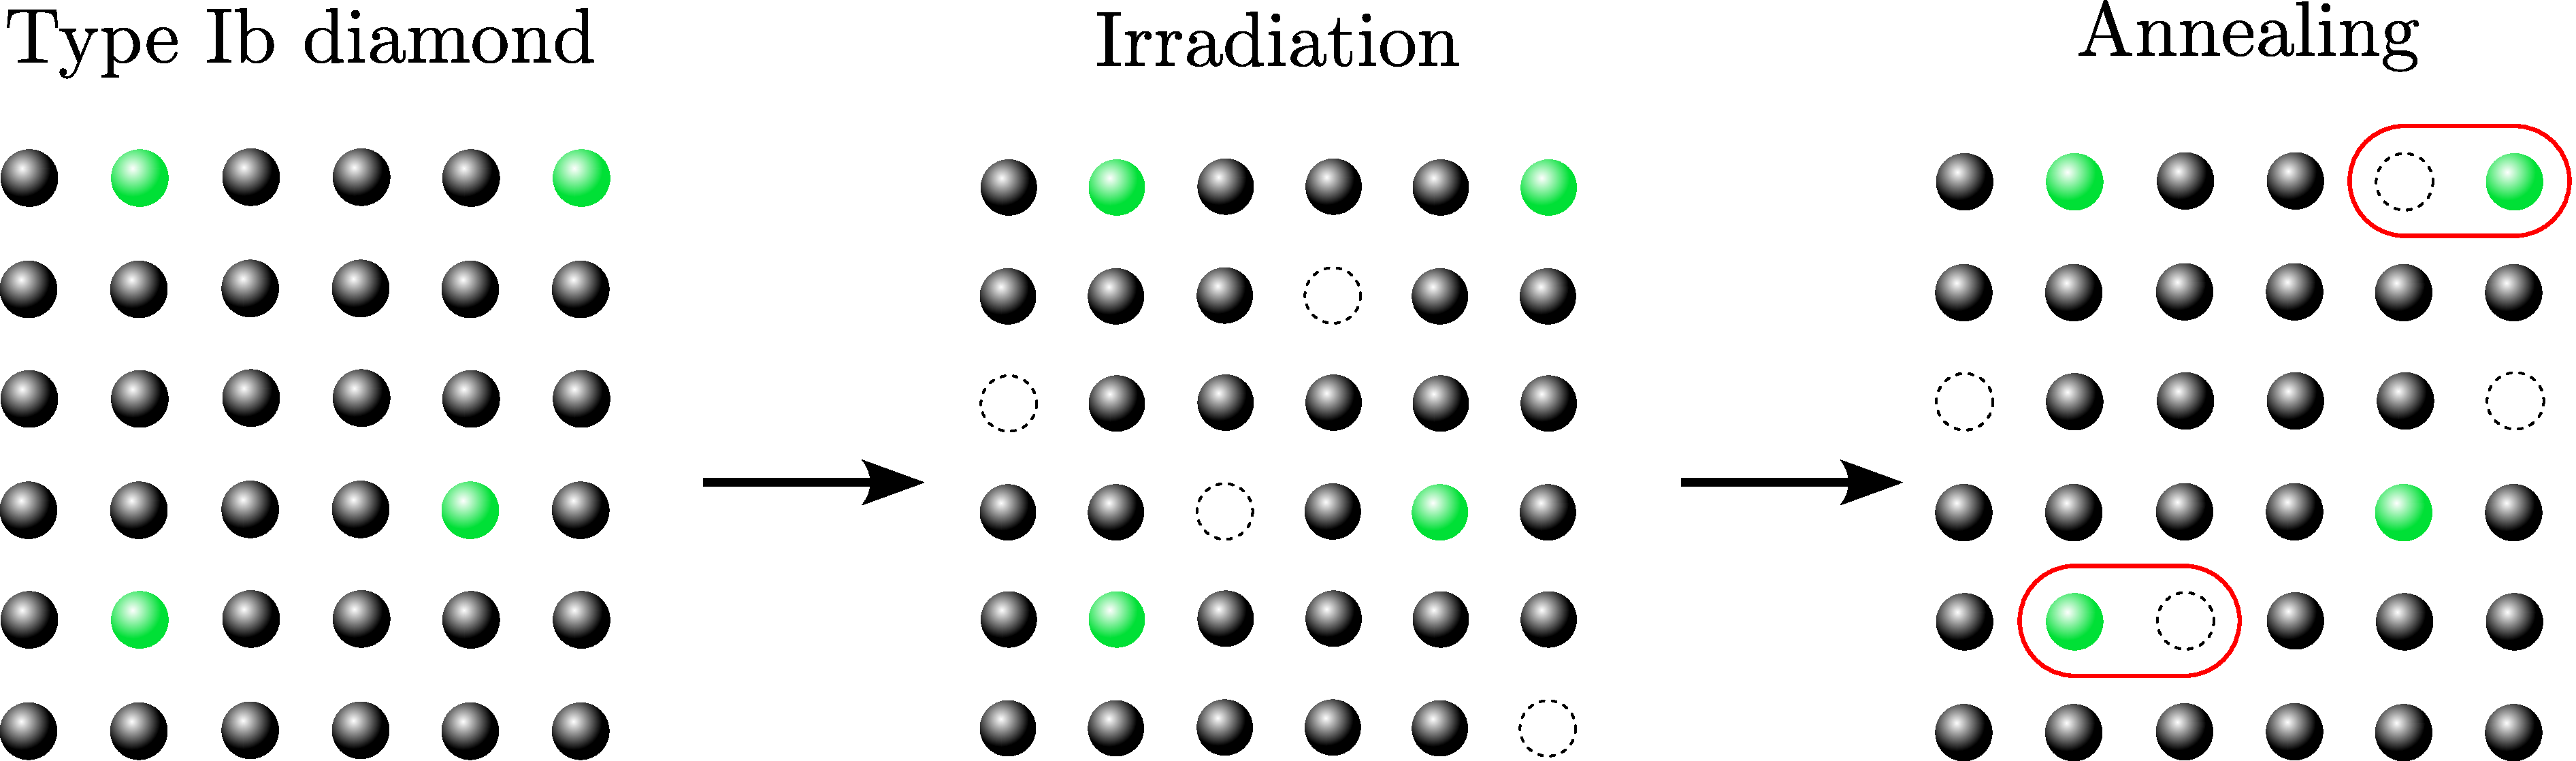
\includegraphics[width=\textwidth]{chapter 1/Figures/formtion_NV_2}
\caption{Illustration of the formation of NV centers. Black and green dots represents carbon and nitrogen atoms respectively}
\label{formation NV}
\end{figure}

NV centers are a relatively rare impurity in untreated diamonds. In CVD diamond for instance, the proportion of nitrogen atoms forming an NV center in an untreated crystal is at best of $2-3 \%$ \citep{hartland2014study}. While this ratio can be enough  to work with single NV centers, applications that require dense ensemble need a higher conversion rate. We will discuss here the usual techniques employed to improve the formation of NV centers.

Fig. \ref{formation NV} illustrates the steps needed to maximize the number of NV centers in the crystal while keeping a relatively high crystalline purity.

The first step to create NV centers is to get individual substitutional N atoms in the crystal ($N_s$, C-centers or P1 centers depending on the literature). This can be achieved either \textit{in situ} by introducing (voluntarily or not) nitrogen in the crystal during the growth process \citep{tallaire2006characterisation, lobaev2017influence}, or \textit{ex situ} by implanting N$^+$ ions with ion implantation techniques \citep{meijer2005generation, smith2019colour}. Because this present work focuses on dense NV ensembles, we will consider the simplest case where the starting crystal is a type-Ib diamond because of the presence of nitrogen during the growth. A starting concentration [N$_s$]= $10 \sim 300$ ppm is typical for type Ib HPHT diamonds \citep{achard2020chemical}.

The second step is to create monovacancies in the crystal lattice. This step might be optional for crystals which already contain a large number of monovacancies, but CVD crystals in particular can have less vacancies that they have substitutional nitrogen atoms \citep{mainwood1999point}. The general technique to create monovacancy is to bombard the sample with high energy particle in order to knock carbon atoms out of the crystal. Several high energy particles have been used to create vacancies, such as protons, electrons, ions, neutrons and even gamma rays \citep{davies1976optical, ashbaugh1988gemstone, kleinsasser2016high}. The most common irradiation source for for bulk diamond however is electron irradiation (e-beam) \citep{acosta2009diamonds}, thanks to their higher availability (compared to neutrons or gamma rays) and their ability to deeply penetrate the crystal.

The final step is to move the vacancies next to the nitrogen atoms. The activation energy required to move vacancy is of $\sim 2.3\ \rm eV$ which corresponds to temperatures of $600\sim 700 ^\circ$C \citep{davies1992vacancy, newton2002recombination}. The most common method to move the vacancies is therefore to anneal the crystal at a temperature $800 \sim 1200 ^\circ$C for a few hours \citep{botsoa2011optimal}. When the vacancy is next to a nitrogen atom, it will only become mobile again for temperatures of $1400 \sim 1500 ^\circ$C \citep{zaitsev2013optical, pinto2012diffusion} which explains why the annealing process favors NV creation.

The final N$_s$ to NV conversion rate can be as high as $\sim 50 \%$ \citep{grezes2015storage, hartland2014study}, although this ratio tends to decrease for higher [N$_s$] concentrations. Most sample studied in this manuscript had a concentration $[\rm NV]= 1-10\ \rm ppm$ (see sample details in Appendix \ref{Appendix samples})

%\subsection{Controlling the NV center charge state}
%
%The charge state of the NV center is of crucial importance for NV applications. Only the negatively charged NV$^-$ center shows the specific spin properties that will be detailed below, but the NV center can exist under three charge states in the diamond: NV$^-$, NV$^0$ and NV$^+$. The presence of NV$^+$ is usually marginal \citep{hauf2014addressing, pfender2017protecting} and we will focus here solely on the NV$^-$ and NV$^0$ charge state.
%
%The charge state of the NV centers depends not only on the growth process of the crystal, but also on the experiment performed with the sample. In particular, illumination in the optical range can promote electrons in the conduction band or holes in the valence band and modify the charge state of the NV center.
%
%On the material side, the crystal has to remain electrically neutral which means that at least as many charge donors need to be present as there are NV$^-$ centers. For nitrogen-rich samples, the donors are mostly N$^+$ centers, which imposes a limit on the maximum conversion rate of N to NV in order to keep a high [NV$^-$]/[NV$^0$] ratio. The possibility to introduce other donors, such as phosphorus, has been studied \citep{doi2016pure} but remains impractical so far \citep{barry2020sensitivity}.
%
%On the experimental side, it has been shown that the ionization of NV$^-$ to NV$^0$ and the reverse process depend on the intensity and wavelength of the laser used for illumination \citep{aslam2013photo}. It was found that the optimal wavelength to preserve the NV$^-$ charge state was  $510-540\ \rm nm$. The most common wavelength used with NV centers is 532 nm (green) due to the historical importance of Nd:YAG lasers. On the other hand, it is possible to semi-permanently ionize the NV$^-$ into NV$^0$ when using a red excitation, which has been used to create optical memories \citep{dhomkar2016long}.
%
%For samples in high excess of [N$_s$] such as type Ib HPHT diamonds, the question of the charge state of the NV center is of relatively low importance as the NV$^-$ state is the predominant one. For sample with a lower [N$_s$] content and a higher [NV]/[N$_s$] ratio however, one must be more careful with the optical intensity and wavelength used as the concentration of NV$^0$ can reach up to 50\% of the total NV concentration \citep{grezes2015storage}

\section{The NV$^-$ center optical and spin properties}

This section focuses on the NV$^-$ center properties both as an optical defect (colored center) and as a spin defect, and compare them to other solid state systems. It also covers the interplay between the spin and the optical levels, a property almost unique to the NV$^-$ center which is the basis for optical polarization and readout of the NV$^-$ spin state.

\subsection{NV center molecular orbitals}

\begin{figure}[h!]
\centering
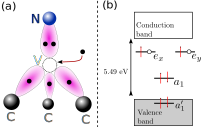
\includegraphics[width=0.8\textwidth]{chapter 1/Figures/NV_electrons}
\caption{(a) Representation of the nitrogen and carbon orbitals surrounding the vacancy of an NV center. Each black dot represents an electron. A sixth electron is required to form the negatively charged NV$^-$ state. (b) Molecular orbitals of the NV center predicted from the the $C_{3v}$ symmetry of the defect. The electron occupation of the NV$^-$ ground state is represented by red arrows.}
\label{NV electrons}
\end{figure}

We will first cover the molecular aspect of the NV defect in diamond and the energy levels of the defect predicted from group theory and ab initio computations.

Fig. \ref{NV electrons}-a) illustrates the $sp^3$ orbitals of the carbons and nitrogen atoms neighboring the vacancy, as well as the 5 electrons occupying dangling bonds from these atoms and a sixth electron captured to form the negatively charged NV$^-$ state. 

Fig. \ref{NV electrons}-b) shows the predicted molecular orbitals of the NV centers, initially computed as linear combination of the $sp^3$ orbitals respecting the $C_{3v}$ symmetry of the defect \citep{loubser1978electron}. This model has since been confirmed by ab initio computation and experimental observations \citep{doherty2013nitrogen}. In particular ab initio computations have shown that the molecular orbitals of the NV center are mostly localized on the nearest neighbors of the vacancy \citep{gali2008ab}. Ab initio computation has also determined that the $a'_1$ level lies in the valence band and is thus often ignored.

The electron occupations shown in Fig. \ref{NV electrons}-b) corresponds to the electronic ground state of the NV$^-$ charge state.

In the remaining part of this manuscript, we will only consider the negatively charged NV$^-$ state, unless specified otherwise. We will therefore omit the ``$-$" from now on and simply refer to the negatively charged state as ``NV".
\subsection{Optical properties of the NV center}
\begin{figure}[h!]
\centering
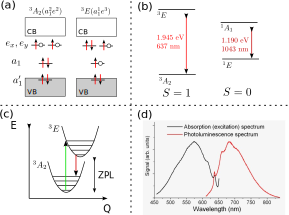
\includegraphics[width=1\textwidth]{chapter 1/Figures/NV_optical}
\caption{Optical properties of the NV center. (a) Electron occupation of the molecular orbitals for the electronic ground state $^3A_2$ and the first excited state $^3E$. (b) Diagram of the main optical transition between the two spin triplet states and of the IR transition between the two singlet sates. The value of the transition corresponds to the zero phonon line (ZPL) and are taken from \citep{doherty2013nitrogen}. (c) Representation of the vibronic structure for the $^3A_2$ and $E^3$ states under the Franck-Condon approximation. The graph axes are the energy of the states $E$ and configuration coordinate $q$. The green and red arrow represents non-resonant (Stokes) absorption and emission processes. (d) Emission and absorption spectrum of the NV center main transition at 300 K, from PL and PLE measurements respectively. Credits: Wikimedia commons}
\label{NV optical}
\end{figure}

Because the NV center has discrete electronic transitions inside the diamond band gap, it fluoresces: it can absorb light from $450-650$ nm and re-emit light in the $600-800$ nm band.

Fig. \ref{NV optical}-a) shows the electronic ground state $^3A_2$ and first excited state $^3E$, where 1 electron from the $a_1$ molecular orbital is promoted to the $e$ level. Both of these electron occupations have two unpaired electrons, meaning that they can exist either either in a spin triplet state ($S=1$) or a spin singlet state ($S=0$) \footnote{The two singlet states $^1E$ and $^1A_1$ represented in Fig. \ref{NV optical}-b) are both of configuration $a_1^2e^2$ where the two $e$ electrons are either in a the same $e$ orbital, or in an antisymmetric superposition of the two $e$ orbitals \citep{doherty2011negatively}.}. 

Fig. \ref{NV optical}-b) shows the zero phonon line (ZPL) for the main transition of the triplet ($^3A_2$ and $^3E$) and singlet ($^1E$ and $^1A_1$) states. It should be noted that due to an inter system crossing between the $^1E$ and $^3A_2$ levels, excitation or absorption of the singlet transition is only possible with a conjoint excitation of the triplet states. By default, we refer to the NV center photoluminescence (PL) as the emission between the two triplet states.

Fig. \ref{NV optical}-c) illustrates the vibronic structure of the $^3A_2$ and $^3E$ states under the Franck-Condon approximation \citep{gali2011time}. The emission and absorption of light associated with the triplet transition can be accompanied by the emission or absorption of an optical phonon. Because the lifetime of the optical phonons is very short, the absorption or emission of light almost always starts from the fundamental state of the $^3A_2$ and $^3E$ level, which explains why the absorption of light can only be done for energies above the ZPL, and the emission for energies below the ZPL (Stokes process).

Finally Fig. \ref{NV optical}-d) shows the absorption and emission spectrum of NV centers at 300 K. A weak zero-phonon-line is visible at 637 nm, with large phonon sidebands in emission and absorption.

\medskip
Compared to similar solid state photon sources (other color centers, quantum dots, dye molecules...), the NV center offer several advantages. First, they are very bright thanks to the $\sim 11\ \rm ns$ lifetime of the excited state and thanks to a quantum efficiency of $0.7-0.8$ \citep{schirhagl2014nitrogen}. With modern nanophotonics methods (solid immersion lenses or diamond waveguide) the PL collected from a single NV center can reach a few $10^6$ photons/s \citep{schroder2016quantum}. Secondly, the NV center is also extremely photostable under green excitation, and does not show any photobleaching \citep{brouri2000photon}. Finally, the diamond itself is resistant to heat and chemical attacks, and presents low toxicity for biologic systems \citep{fu2007characterization}. There are however drawbacks in using NV centers for photonics applications, the main one being that $\leq 4\%$ of the photons emitted by the NV centers are in the ZPL (low Debye Waller factor), even at cryogenic temperature \citep{johnson2015tunable}. This limits the potential of NV centers for quantum photonic devices \citep{bradac2019quantum}.

\subsection{Spin properties of the NV center electronic ground state}
\begin{figure}[h!]
\centering
\includegraphics[width=1\textwidth]{chapter 1/Figures/spin_fine_hyperfine}
\caption{Representation of the fine and hyper-fine structure of the $^3A_2$ state for a $^{14}$N nucleus and $^{12}$C nuclei.}
\label{NV spin}
\end{figure}

We will only focus here on the spin structure of the electronic ground state $^3A_2$, as the lifetime of the other states is too short to make effective spin qubits. All the numerical values in this section were found in \citep{smeltzer2009robust, doherty2013nitrogen} and the references within.

The spin structure in the ground state consists in an electronic spin $S=1$ coupled to the nuclear spin of the nearby nuclei. Carbon's most common isotope is $^{12}$C at 98.9 \% natural abundance. $^{12}$C has a a nuclear spin $I=0$ and therefore does not contribute to the hyper-fine structure. Nitrogen's most common isotope however is $^{14}$N at 99.6 \% natural abundance which has a nuclear spin $I=1$ and does create a hyper-fine splitting. We will only cover here the most likely configuration for an NV center which is a $^{14}$N nucleus and $^{12}$C nuclei as closest neighbors. 

The spin system considered is then an electronic spin $S=1$ coupled to a nuclear spin $I=1$ with a Hilbert space of dimension $(2S+1)(2I+1)=9$. The spin Hamiltonian of the system can be written:
\begin{equation}
\mathcal{H}=\mathcal{H}_e + \mathcal{H}_n + \mathbf{S}\cdot \bar{\bar{A}}\cdot \mathbf{I},
\end{equation}
where $\mathcal{H}_e$ is the purely electronic spin Hamiltonian, $\mathcal{H}_n$ the purely nuclear spin Hamiltonian, $\mathbf{S}$ the electronic spin operator, $\mathbf{I}$ the nuclear spin operator and $\bar{\bar{A}}$ the hyper fine tensor.
\subsubsection{Electronic spin Hamiltonian}
The electronic spin Hamiltonian $\mathcal{H}_e$ can be written:
\begin{equation}
\label{eq. spin elec}
\mathcal{H}_e=D S_z^2 + \gamma_e \mathbf{S} \cdot \mathbf{B} + \mathcal{H}_{elec}(\mathbf{E})+ \mathcal{H}_{strain}(\mathbf{\bar{\bar{\varepsilon}}}).
\end{equation}

The term $D S_z^2$ corresponds to the fine structure of the electronic spin. It originates from the dipole-dipole coupling between the two unpaired electrons of the defect. Due to the strong anisotropy of the molecular orbitals of the defect, the fine structure term imposes the quantization axis $\mathbf{z}$ (via the $S_z$ operator) where $\mathbf{z}$ is the direction of the N$-$V axis in the diamond. $D$ is called the zero field splitting (ZFS) factor and its value is $D\approx 2.87\ \rm GHz$ at 300 K.

$\gamma_e \mathbf{S} \cdot \mathbf{B}$ is the Zeeman splitting of the spin, where $\gamma_e \approx 2.8\ \rm MHz/G$ is the gyromagnetic ratio of the electronic spin (almost equal to that of a free electron in the case of the NV center).

$\mathcal{H}_{elec}$ and $\mathcal{H}_{strain}$ are the dependency of the Hamiltonian on the electric field and crystal strain and will be discussed in further details in chapter 4.

\subsubsection{Nuclear spin Hamiltonian and hyperfine coupling}
The nuclear spin $\mathcal{H}_n$ can be written:
\begin{equation}
\mathcal{H}_e=Q I_z^2 + \gamma_n \mathbf{I} \cdot \mathbf{B},
\end{equation}

where $Q=-4.945\ \rm MHz$ is the nucleus electric quadrupole moment and $\gamma_n=-0.308\ \rm kHz/G$ is the nuclear gyromagnetic ratio.

Finally the hyper-fine tensor can be written diagonally:
\begin{equation}
\bar{\bar{A}} = \begin{pmatrix}
A_{xx} & 0 & 0 \\
0 & A_{yy} & 0 \\
0 & 0 & A_{zz}
\end{pmatrix},
\end{equation}
where $A_{zz}=-2.162\ \rm MHz$ and $A_{xx}=A_{yy}=-2.62\ \rm MHz$. The $z$ direction in the electronic spin Hamiltonian, the nuclear spin Hamiltonian and the hyper-fine tensor awlays refer to the direction of the N$-$V axis.

Fig. \ref{NV spin} shows fine and hyper-fine structure of the NV center without any external fields.

The hyper-fine splitting as well as the electric and strain dependency are of second order compared to the Zeeman and zero field splitting terms. Unless specified otherwise, we will from now on refer to the following simplified Hamiltonian as the NV spin Hamiltonian:

\begin{align}
\label{NV spin Hamiltonian basic}
\mathcal{H}&=D S_z^2 + \gamma_e \mathbf{S} \cdot \mathbf{B} \\
&=\begin{pmatrix}
D-\gamma_e B_z & \frac{\gamma_e (B_x+iB_y)}{\sqrt{2}} & 0 \\
\frac{\gamma_e (B_x-iB_y)}{\sqrt{2}} & 0 & \frac{\gamma_e (B_x+iB_y)}{\sqrt{2}} \\
0 & \frac{\gamma_e (B_x-iB_y)}{\sqrt{2}} & D+\gamma_e B_z
\end{pmatrix}
\end{align}

\bigskip
The NV center's spin use as a qubit is prevalent in quantum communication \citep{wehner2018quantum}, quantum computing \citep{de2021materials} and quantum sensing \citep{degen2017quantum}. Part of the reason for this wide usage are the overall long relaxation times (lifetime $T_1$ and coherence time $T_2$) of the order of a few ms at room temperature \citep{balasubramanian2009ultralong}, as well as the ability to address individual nuclear spins with even longer relaxation times \citep{awschalom2018quantum}. However the main advantage of the NV center spin compared to other solid state spin qubits is its ability to be polarized and read-out optically thanks to the properties detailed in the following section.


\subsection{Intersystem crossing of the electronic levels}
\label{sec ISC}
\begin{figure}[h!]
\centering
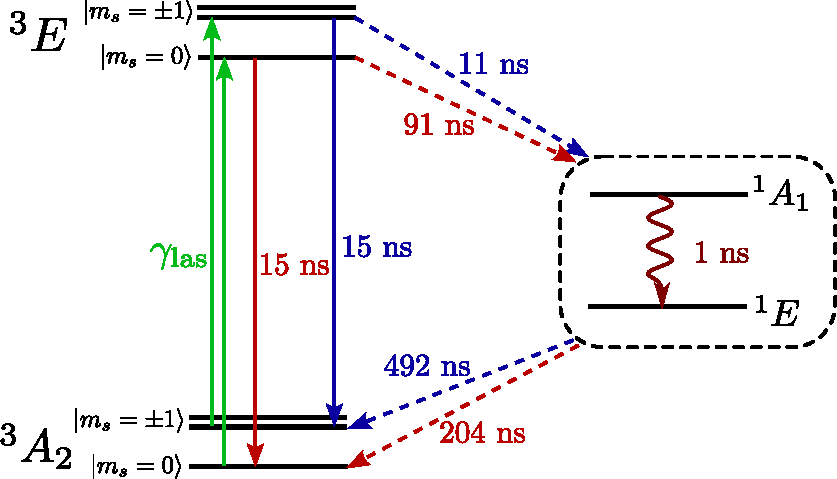
\includegraphics[width=0.8\textwidth]{chapter 1/Figures/ISC}
\caption{Inter system crossing of the NV center. Blue arrows symbolize decay channels to and from the $\ket{m_s=\pm 1}$ states and red arrows the decay channels to and from the $\ket{m_s=0}$ states. Green arrows symbolize the optical excitation induced by the laser. The indicated durations correspond to the inverse of the decay rates found in \citep{gupta2016efficient}.}
\label{ISC}
\end{figure}

The optical excitation and radiative decay between the $^3A_2$ and $^3E$ levels preserve the spin projection $m_s$ \citep{robledo2011spin}. There is however a non-radiative decay path which involves an inter-system crossing with the singlet states $^1A_1$ and $^1E$ that depends on the the triplet states spin projection.

Fig. \ref{ISC} summarizes the possible decay channels from the $^3E$ states. Once excited to the $^3E$ states, for instance by photoexcitation, the electrons can either decay radiatively and emit a 600$-$800 nm photon, or undergo an intersystem crossing and decay through the singlet states. The decay though the singlet state is often referred to as non-radiative, due to both the difference in wavelength between the triplet and the singlet transitions, and due to the strong non-radiative competition in the singlet decay (quentum efficiency $\leq 10^{-3}$ \citep{rogers2008infrared, ma2010excited, acosta2010optical}.

The rates $\gamma$ of the various decay processes, represented in Fig. \ref{ISC} by the time constant $\tau=1/\gamma$, strongly depend on the spin projection $m_s$. Importantly, the likeliness to undergo a non-radiative decay is $\sim 4$ times\footnote{$\frac{15+91}{15+11}\approx 4$} more likely when starting from the $\ket{\pm 1}$ states than when starting from the $\ket{0}$ state. Similarly, the singlet state is $\sim 2.4$ times\footnote{$\frac{492}{204} \approx 2.4$} more likely to decay to the $\ket{0}$ state than to the $\ket{\pm 1}$ states.

These spin selective intersystem crossings mean that an optical pumping scheme in the $\ket{m_s=0}$ spin state takes place under constant green excitation. At optical saturation, the polarization of the $\ket{0}$ state can reach $70-90\ \%$ \citep{gupta2016efficient}. This is equivalent to a spin-temperature $\approx 65\ \rm mK$ \footnote{\begin{equation*}
T=\frac{h D}{k_B \ln (\frac{1-P}{2P})} \approx 65\ \rm mK,
\end{equation*}
where $D$ is th ZFS factor described in eq. (\ref{eq. spin elec}) and $P\approx 0.8$ is the spin polarization defined as the population in the $\ket{0}$ state.}.

Another effect of the intersystem crossing is the ability to optically readout the spin state of the NV center: since the $\ket{0}$ state is more likely to undergo a radiative decay than the $\ket{\pm 1}$ states, the expected photoluminescence (PL) is higher when starting from the $\ket{0}$ state than a $\ket{\pm 1}$ state. While the $\ket{+1}$ and $\ket{-1}$ states cannot be a priori distinguished, a direct excitation of the $\ket{+1} \to \ket{0}$ or $\ket{-1} \to \ket{0}$ transition with a resonant microwave can unambiguously reveal the initial spin state.

It should be noted that the decay rates indicated in Fig. \ref{ISC} cannot be directly measured. They have to be inferred from the PL dynamics at short times after illumination. Different experiments and different models have thus lead to different decay rates \citep{duarte2021effect}. 

\section{Dipole-dipole interaction between two electronic spins}

\begin{figure}[h!]
\centering
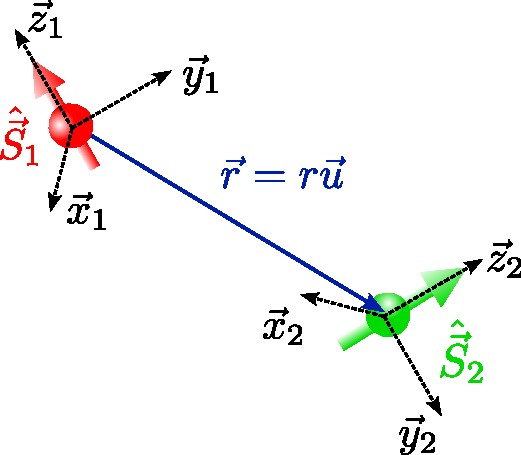
\includegraphics[width=0.4\textwidth]{chapter 1/Figures/shema_dipole_dipole}
\caption{Geometric representation of two interacting spins. ($\mathbf{x}_1,\mathbf{y}_1,\mathbf{z}_1$) and ($\mathbf{x}_2,\mathbf{y}_2,\mathbf{z}_2$) represent Cartesian coordinate systems in the spin frames of reference, where $\mathbf{z}_i$ is the axis of quantization of spin $i$.} 
\label{dipole-dipole}
\end{figure}

This final introductory section will focus on the dipole-dipole interaction between two electronic spins, which is the main form of spin-spin interaction and plays a key part in the properties of dense spin ensemble. 

We will consider the general situation represented in Fig. \ref{dipole-dipole}: two spins separated by a distance $r$ with their own coordinate systems ($\mathbf{x}_1,\mathbf{y}_1,\mathbf{z}_1$) and ($\mathbf{x}_2,\mathbf{y}_2,\mathbf{z}_2$). The coordinate system is chosen so that each spin operator can be written:

\begin{equation}
\hat{\mathbf{S}}_i=\hat{S}_x \mathbf{x}_i + \hat{S}_y \mathbf{y}_i + \hat{S}_z \mathbf{z}_i
\end{equation}

where the spin operators $\hat S_{\{x,y,z\} }$ have their usual definitions in term of Pauli matrices. In particular, this means that the spin axis of quantization of each spin is $z_i$, which classically corresponds to the magnetization direction of the dipole. This axis can be defined either by the magnetic field, or by crystal field anisotropies, as is often the case for solid state spins with $S\geq 1$ (including the NV center).

\subsection{Magnetic dipole-dipole Hamiltonian}

Classically, the dipole-dipole interaction between two magnetic moments $\mathbf{m}_1$ and $\mathbf{m}_2$ can be derived by computing the static magnetic field generated by one dipole at the position of the second dipole \cite[p.~188]{jackson1999classical}:

\begin{align}
U&=-\mathbf{m}_1 \cdot \mathbf{B}(\mathbf{r}) \nonumber \\
&=-\frac{\mu_0}{4 \pi}\left[ \frac{3 (\mathbf{m}_1\cdot\mathbf{u})(\mathbf{m}_2\cdot\mathbf{u}) - \mathbf{m}_1\cdot\mathbf{m}_2}{r^3}+\frac{8\pi}{3}\mathbf{m}_1\cdot\mathbf{m}_2\,\delta(r)\right], \label{eq. dipole classique}
\end{align}

where $\mathbf{r}=r \mathbf{u}$ is the relative position of the two dipoles (see Fig. \ref{dipole-dipole}). 

The quantum analog of the dipole-dipole interaction between spins simply replaces the magnetic moments $\mathbf{m}_i$ in eq. (\ref{eq. dipole classique}) with $\hbar \gamma_i \hat{\mathbf{S}}_i$, where $\gamma_i$ is the gryromagnetic ratio and $\hat{\mathbf{S}}_i$ the spin vector operator for spin $i$:

\begin{equation}
\label{eq. dipole quantique J coupling}
\mathcal{H}_{\rm dd}=\frac{\mu_0 \gamma_1 \gamma_2 \hbar^2}{4 \pi}\left[ \frac{3 (\hat{\mathbf{S}}_1\cdot\mathbf{u})(\hat{\mathbf{S}}_2\cdot\mathbf{u}) - \hat{\mathbf{S}}_1\cdot\hat{\mathbf{S}}_2}{r^3}+\frac{8\pi}{3}\hat{\mathbf{S}}_1\cdot\hat{\mathbf{S}}_2\,\delta(r)\right].
\end{equation}

The $\delta(r)$ term represents the Fermi contact energy. This term plays an important role when there is an overlap of the spin particle wavefunctions, such as the hyperfine coupling between the NV$^-$ electron spin and $^{14}$N \cite{doherty2012theory} or  $^{13}$C \cite{smeltzer201113c} nuclear spins.

The focus of this manuscript is on the interaction between electronic spins which are separated by several atomic sites (density impurities in the $\sim$ ppm range). We will therefore assume that there is negligible overlap between the electronic wavefunctions and omit the Fermi contact term. This leads the simplified dipole-dipole Hamiltonian:

\begin{equation}
\mathcal{H}_{\rm dd}= \frac{J_0}{r^3}\left[ 3 (\hat{\mathbf{S}}_1\cdot\mathbf{u})(\hat{\mathbf{S}}_2\cdot\mathbf{u}) - \hat{\mathbf{S}}_1\cdot\hat{\mathbf{S}}_2] \right],
\end{equation}

where $J_0=\frac{\mu_0 \gamma_1 \gamma_2 \hbar^2}{4 \pi}$.

For two electronic spins with $g$-factors $\approx -2$\footnote{Most spin defects in diamond, including the NV center have a g-factor $\approx -2$ similarly to free electrons.}, 
\begin{equation*}
\frac{J_0}{h} \approx 51.8\ \rm{MHz}\cdot \rm{nm}^3.
\end{equation*}

\subsection{Decomposition of the dipole-dipole Hamiltonian}
\label{sec flip-flop et double flip}

\begin{figure}[h!]
\centering
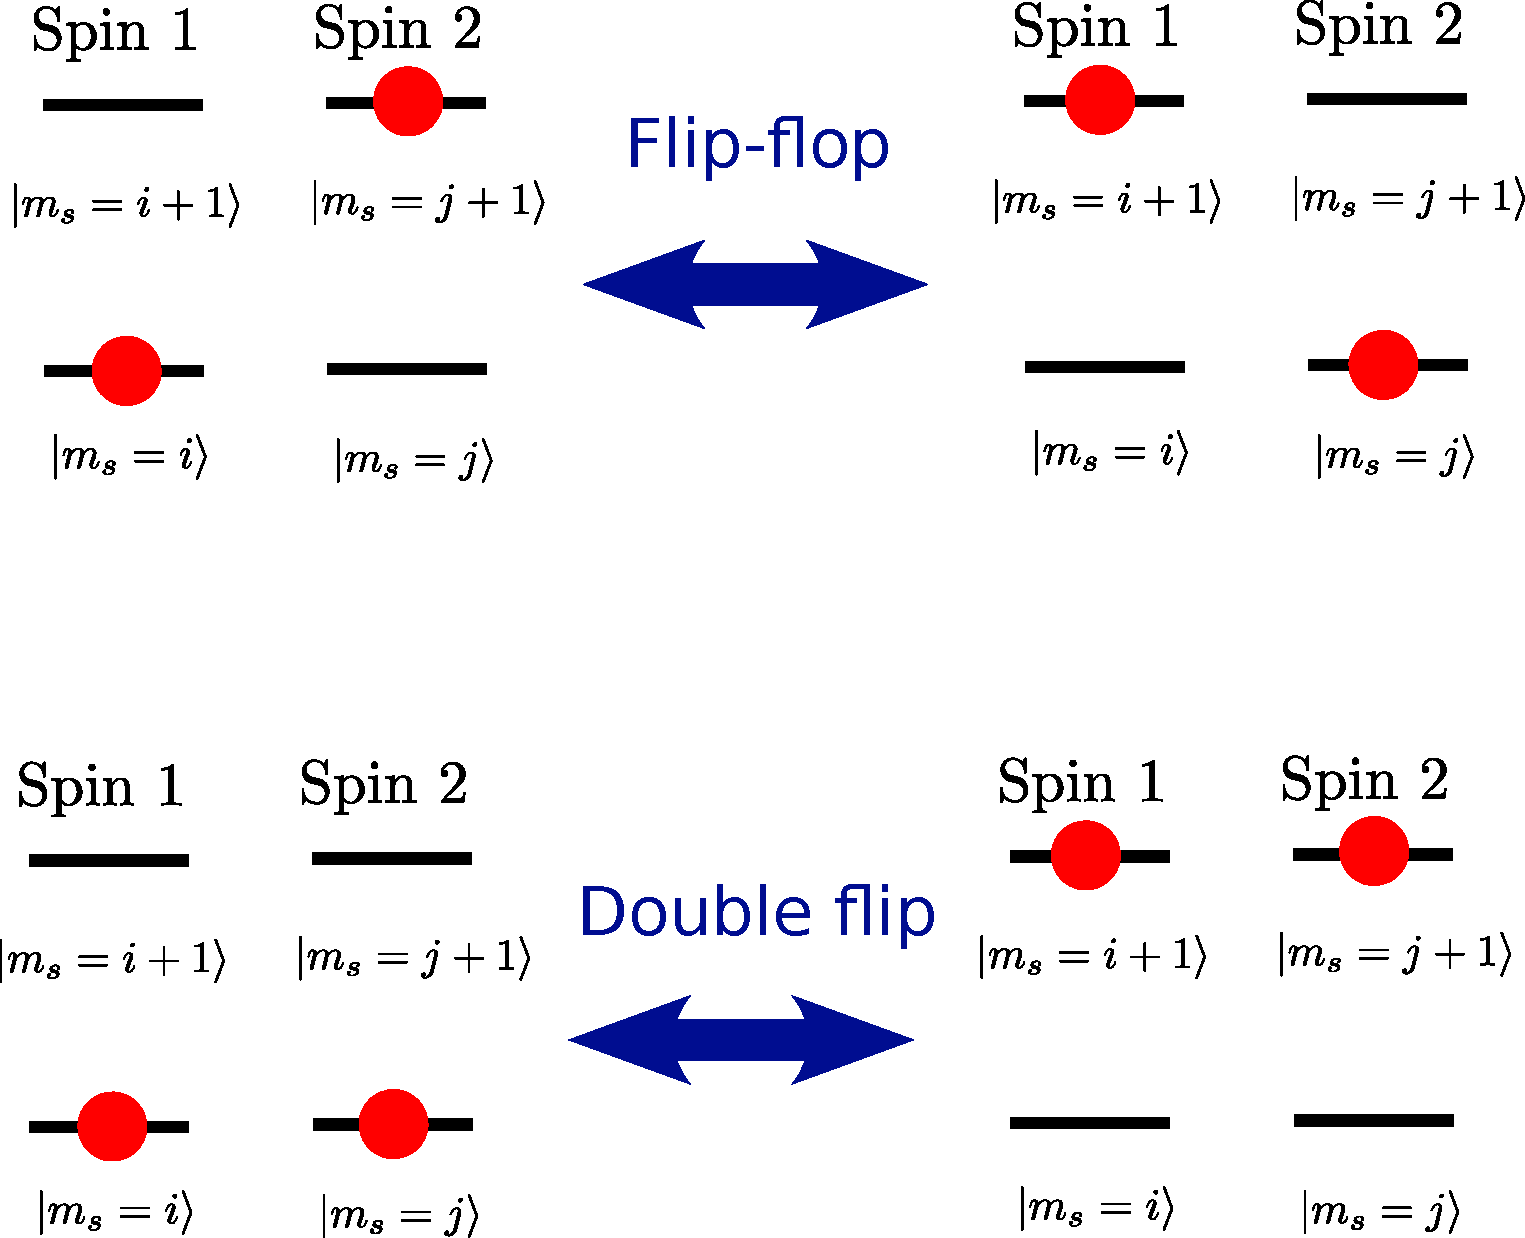
\includegraphics[width=.7\textwidth]{chapter 1/Figures/flip-flop_double-flip}
\caption{Representation of the two energy transfer mechanisms: flip-flop and double flips} 
\label{flip flop double flip}
\end{figure}

In the weak coupling approximation, the dipole-dipole Hamiltonian between two spins can be decomposed between diagonal terms which are responsible for energy shifts of the individual spin levels, and the off-diagonal terms which are responsible for energy transfers between the two spins.

In what follows, we will assume that both spins have the same quantization axis in order to simplify the Hamiltonian decomposition. A more general case is detailed in appendix \ref{Appendix eta}.

Following the notation introduced in Fig. \ref{dipole-dipole}, we will then assume that $$(\mathbf{x}_1,\mathbf{y}_1,\mathbf{z}_1) = (\mathbf{x}_2,\mathbf{y}_2,\mathbf{z}_2) = (\mathbf{x},\mathbf{y},\mathbf{z}).$$ We will denote $\mathbf{u}=u_x \mathbf{x} + u_y \mathbf{y} + u_z \mathbf{z}$ the decomposition of the unitary vector $\mathbf{u}$ in this basis. The dipole-dipole Hamiltonian can then be written:
\begin{equation}
\mathcal{H}_{\rm dd}=\frac{J_0}{r^3}\left[ (3 u_x^2-1) S_x^1 S_x^2 + (3 u_y^2-1) S_y^1 S_y^2 + (3 u_z^2-1) S_z^1 S_z^2 \right],
\end{equation}
where $S_{\{x,y,z\} }^i$ are the spin operators acting on spin $i$. The $S_z^1 S_z^2$ term is the only diagonal term and corresponds to energy shifts while the $S_x^1 S_x^2$ and $S_y^1 S_y^2$ terms are responsible for energy transfer. To make the transfer mechanism more apparent, we will rewrite $S_x^i$ as $\frac{1}{2}(S_+^i+S_-^i)$ and $S_y^i$ as $\frac{1}{2i}(S_+^i-S_-^i)$:
\begin{align}
\mathcal{H}_{\rm dd}&=\frac{J_0}{r^3}\bigg{[} \frac{1}{4}(3 u_x^2 + 3 u_y^2 -2)(S_+^1 S_-^2 + S_-^1 S_+^2) \nonumber \\
&\quad + \frac{1}{4}(3 u_x^2 - 3 u_y^2)(S_+^1 S_+^2 + S_-^1 S_-^2) \nonumber \\
&\quad +(3 u_z^2-1) S_z^1 S_z^2 \bigg{]} \nonumber \\
\medskip
&= \Omega_{\rm ff} (S_+^1 S_-^2 + S_-^1 S_+^2) + \Omega_{\rm df} (S_+^1 S_+^2 + S_-^1 S_-^2) + \Omega_{\rm shift} S_z^1 S_z^2. \label{eq. ff df}
\end{align}

We have introduced in eq. (\ref{eq. ff df}) the three relevant matrix elements $\Omega_{\rm ff}$, $\Omega_{\rm df}$, and $\Omega_{\rm shift}$ which correspond respectively to flip-flops, double flips and energy shifts. Flip-flops and double flips (sometimes referred as flip-flips) are represented in Fig. \ref{flip flop double flip}. Flip flops correspond to energy transfer between two spins for which the sum of the spin angular momentum is conserved ($\Delta (m_s^1+m_s^2)=0$), while double flips correspond to energy transfer for which the spin angular momentum is not conserved ($\Delta (m_s^1+m_s^2)=\pm 2$)\footnote{In order to preserve the total angular momentum, double flips transfer angular moment to the crystal, which is a form of Einstein de Haas effect \citep{einstein1915experimental} }. In both cases however, the energy between the initial and final states needs to be preserved for the transfer to be efficient. 

It should be noted that on average, each matrix element is of the same order of magnitude: $\Omega_{\rm ff} \sim \Omega_{\rm df} \sim \Omega_{\rm shift} \sim \frac{J_0}{r^3}$. 

\subsection{Cross-relaxations with NV centers}
\label{Sec_CR}
\begin{figure}[h]
\centering
\includegraphics[width=0.9\textwidth]{chapter 1/Figures/Shema_CR}
\caption{Illustration of cross-relaxations between an NV center and an unpolarized spin. Red dots represent the population in each states, and the arrows the various population transfer mechanisms}
\label{CR_shema}
\end{figure}

Cross-relaxation (CR) is the transfer of polarization from one spin to another (or more generally from one family of spins to another family). This process can occur through either flip-flops or double flips, as long as the resonance condition between the two spins is met. 

On of the condition for cross-relaxation is to have a difference in polarization between the two spins species considered. The NV center is therefore a good candidate to observe cross-relaxations as it can be optically polarized while most other spin species are not. 

Fig. \ref{CR_shema} illustrates CR between a polarized NV center and an unpolarized second spin. When the two considered spin transitions become resonant, in this case by tuning the magnetic field, polarization from the NV center will be transferred to the second spin, making the NV center less polarized and the second spin more polarized than when they are out of resonance. 

For a single NV center coupled to spin 2, assuming that spin 2 always remains depolarized\footnote{This is the case in practice if the spin 2 bath is much bigger than the NV bath and effectively acts as a thermostat, or if the lifetime of spin 2 is much smaller than that of the NV center.} and that the coupling strength between the two spins is smaller than their respective dephasing time $T_2^*$ (weak coupling regime), the modification in the NV relaxation rate $\Gamma_1=\frac{1}{T_1}$ caused by the cross-relaxation with spin 2 can be analytically computed \citep{hall2016detection}:
\begin{equation}
\delta \Gamma_1=\frac{\Omega^2}{\Gamma_2^*} \frac{(\Gamma_2^*)^2}{(\delta \nu)^2+(\Gamma_2^*)^2},
\label{delta gamma 1}
\end{equation}
where $\Gamma_2^*=\frac{1}{T_2^*(\rm NV)}+\frac{1}{T_2^*(\rm Spin 2)}$ is the joint dephasing rate of the NV center and the second spin, $\delta \nu$ is the detuning in energy (expressed in frequency) between the initial and final states and $\Omega=\Omega_{\rm ff}$ or $\Omega_{\rm df}$ is the dipole-dipole matrix element corresponding to the flip-flop or double-flip process considered. 

Eq. (\ref{delta gamma 1}) is the basis for every cross-relaxation detection performed in this manuscript. Because the NV center lifetime can be measured optically, as detailed in Sec. \ref{sec T1 NV}, cross-relaxation between NV-centers and other spin species can be measured optically. Measuring the cross-relaxation depolarization can then be used to gain information on the second spin or on the dipole-dipole interaction mechanisms, as will be explained in the following chapters.

\section{Optically detected magnetic resonance (ODMR)}

This section introduces one of the building block of almost any NV experiment which is the optically detected magnetic resonance (ODMR). ODMR is used to find the spin resonances of the NV center, which is a preliminary step to any coherent manipulation of the NV spin, as well as a powerful sensing tool in itself.

This section also covers the experimental setup used for this operation and for many other NV experiments, as well as the concept of longitudinal and transverse magnetic field with regard to the NV principal axis.

\subsection{Experimental setup}
\label{Sec setup cahp 1}
\begin{figure}[h!]
\centering
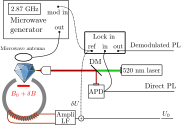
\includegraphics[width=0.8\textwidth]{chapter 1/Figures/shema_exp}
\caption{Confocal microscopy setup (details in main text).}
\label{setup ch1}
\end{figure}
The three most common experimental degrees of freedom to consider for NV experiments are: the optical illumination, the microwave field and the external magnetic field. Other parameters such as the crystal temperature, the electric field or the crystal stress can also be controlled for specific applications.

Fig. \ref{setup ch1} shows a multi-purpose experimental setup which offers a control over these three degree of freedoms. Unless specified otherwise, this is the experimental setup that was used to perform all the measurements shown in this manuscript. 

The setup consists of a confocal microscope where the excitation from a green laser (Thorlabs CPS532, 532 nm, 5 mW) is focused on a sample containing NV centers with a microscope objective (NA $\sim$ 0.5). The NV PL is then collected by the same objective and isolated from the back-scattered laser light with a dichroic mirror (DM) and additional filters (532 nm notch filter and 645 nm longpass filter to filter out the NV$^0$ PL). The PL is collected on an avalanche photodiode (Thorlabs APD410A or Perkin Elmer SPCM-AQRH-15) whose signal is sent to the acquisition card (NI X-series).

The laser beam goes through an acousto-optic modulator (AOM, AA opto-electronic) controlled externally to create arbitrary light pulses (resolution $\sim$ ns). The microwave field is generated by a Rhode \& Shwarz SMB 100A generator and emitted with a home-made loop antenna positioned at $<$ 1 mm of the sample. A microwave switch (Mini-circuits ZASWA-2-50DRA+) is used to create microwave pulses (resolution $\sim$ 10 ns). The control pulses for the AOM and the microwave switch are generated either by the NI X-series card (resolution $\sim$ 1 $\mu$s), or by a pulseblaster ESR-PRO (resolution $\sim$ 10 ns). The microwave field can be amplified with a Mini-circuits ZHL-5W-422+ amplifier to achieve higher Rabi frequencies. 

Finally the magnetic field is generated either with a permanent magnet (up to $\sim$ 200 mT) or with a homemade electromagnet (up to $\sim$ 30 mT) alimented via a low freqency amplifier (Leybold power function generator 522663). Both the permanent magnet and the electromagnet can be  attached to a rotation stage for precise alignment.

The X-series and the pulseblaster, as well as several instruments (microwave generator, motorized stages) are piloted by python scripts which I developed during my PhD.
%Salaud de Gabriel
%\subsection{Rabi Oscillations}
%\begin{figure}[h!]
%\centering
%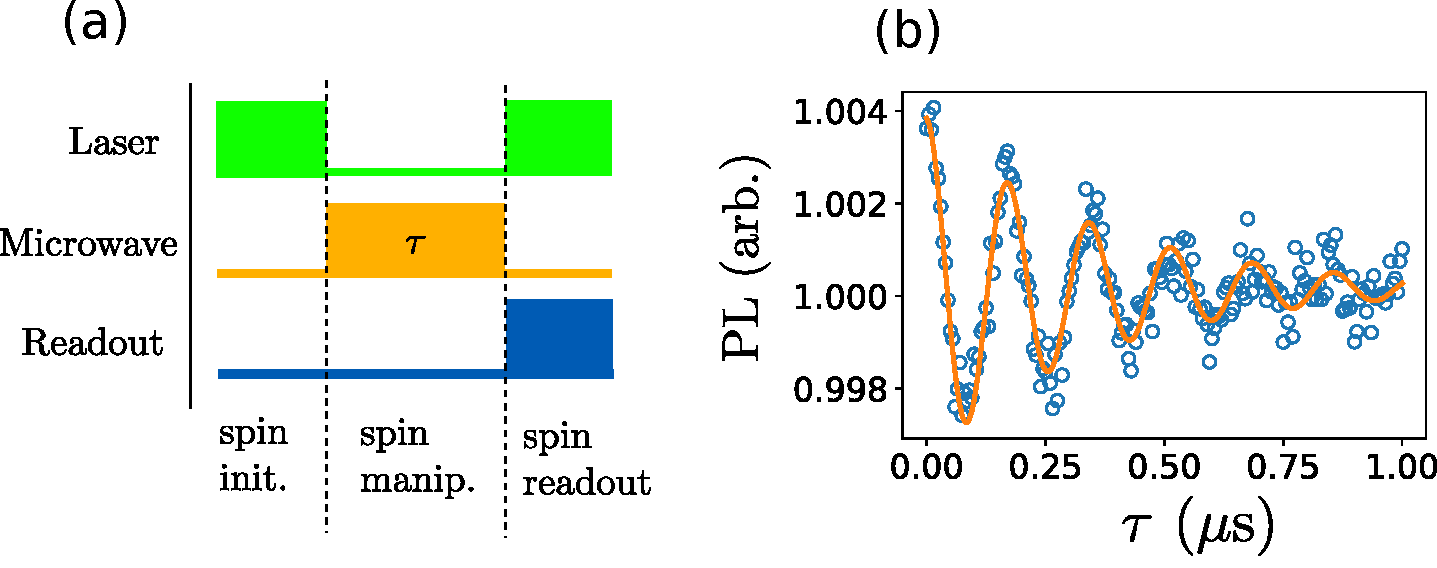
\includegraphics[width=\textwidth]{chapter 1/Figures/Rabi}
%\caption{Rabi oscillations. (a) pulse sequence used to measure Rabi oscillations. (b) Experimental data on sample CVD-pink (see sample details in appendix \ref{Appendix samples}).}
%\label{Rabi}
%\end{figure}
%
%The general technique for experiments involving NV spins proceeds as follow: 
%\begin{itemize}
%\item First the spins are polarized. This is done with a green laser pulse ($1-100$ $\mu$s depending on the laser intensity) which polarizes the spins in the $\ket{m_s=0}$ state at $\sim$ 80 \%.
%\item  Then the spins are manipulated. This process often involves a microwave field resonant with one of the spin transitions.
%\item Finally the spins are read out. The simplest spin readout for NV centers consists in looking at the PL right after the laser is turned on: if the spin was in the $\ket{m_s=0}$ state, the initial PL will be high, whereas if the spin was in a $\ket{m_s=\pm 1}$ state, the initial PL will be low. For longer exposure time, the spins end up re-polarized in the $\ket{m_s=0}$ state and no information can be gained on the initial spin state anymore. The optimal readout time is of the same order as the spin polarization time ($1-100$ $\mu$s).
%\end{itemize}
%
%Fig. \ref{Rabi}-a) shows the pulse sequence used to observe Rabi oscillations with NV centers. In this case, the spins manipulation simply consists in a microwave pulse of variable duration $\tau$. The microwave frequency or the magnetic field needs to be adjusted so that at least one NV spin transition (either $\ket{0} \to \ket{+1}$ or $\ket{0} \to \ket{-1}$) is resonant with the microwave field. 
%
%Fig. \ref{Rabi}-b) shows the result of such an experiment on a spin ensemble. The PL signal oscillations correspond to the oscillations of the spin population between the bright $\ket{0}$ state and the dark $\ket{-1}$ state. For long microwave pulses ($>$ 1 $\mu$s typically), the spins reach a steady state with  $\sim$ 50 \% population in both the $\ket{0}$ and $\ket{-1}$ states.


\subsection{Optically detected magnetic resonance}
\begin{figure}[h!]
\centering
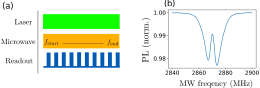
\includegraphics[width=\textwidth]{chapter 1/Figures/ODMR_basique}
\caption{ODMR protocol. (a) Pulse sequence used for CW ODMR: the microwave is kept on during the whole sequence while the frequency is scanned from $f_{\rm start}$ to $f_{\rm end}$. (b) ODMR spectrum with no magnetic field on sample ADM-15-4. (see sample details in appendix \ref{Appendix samples}).}
\label{ODMR basique}
\end{figure}

Optically detected magnetic resonance (ODMR) is the most commonly employed magnetometry protocol with NV centers due to its simplicity and the fact that it does not require prior calibration.

The protocol for continuous wave (CW) ODMR is presented in Fig. \ref{ODMR basique}. In this simple protocol, the microwave is always turned on while the frequency spans a predefined interval $[f_{\rm start}, f_{\rm end}]$. The PL is recorded as the microwave is being swept, with a typical acquisition time for each PL sample $> 1\ \rm ms$. The sweeping frequency must be slow enough so that the PL can reach a steady state with the microwave field for each sample acquisition. 

Whenever the microwave becomes resonant with one of the NV transition, it induces a depolarization of the NV center which results in a drop of PL. This allows an optical reading of the NV spin spectral response. 

Fig. \ref{ODMR basique}-b) shows an example of ODMR spectrum on an NV ensemble with no external magnetic field. The reason as to why there are two peaks instead of a single one centered on $D=2870\ \rm MHz$ is the splitting of the $\ket{+1}$ and $\ket{-1}$ levels occasioned by the strain and local electric field, which will be further discussed in chapter 4. The asymmetry between the two peaks could come either from the microwave polarization or from the uneven spectral response of the antenna \footnote{Our antennas are not impedance matched.}. 

ODMR contrast of up to 30 \% of the PL have been recorded with single spins \citep{dreau2011avoiding}. We typically observe ODMR contrast $\leq 5\ \%$ with NV ensemble.

\subsubsection{ODMR with lock-in detection}
\begin{figure}[h!]
\centering
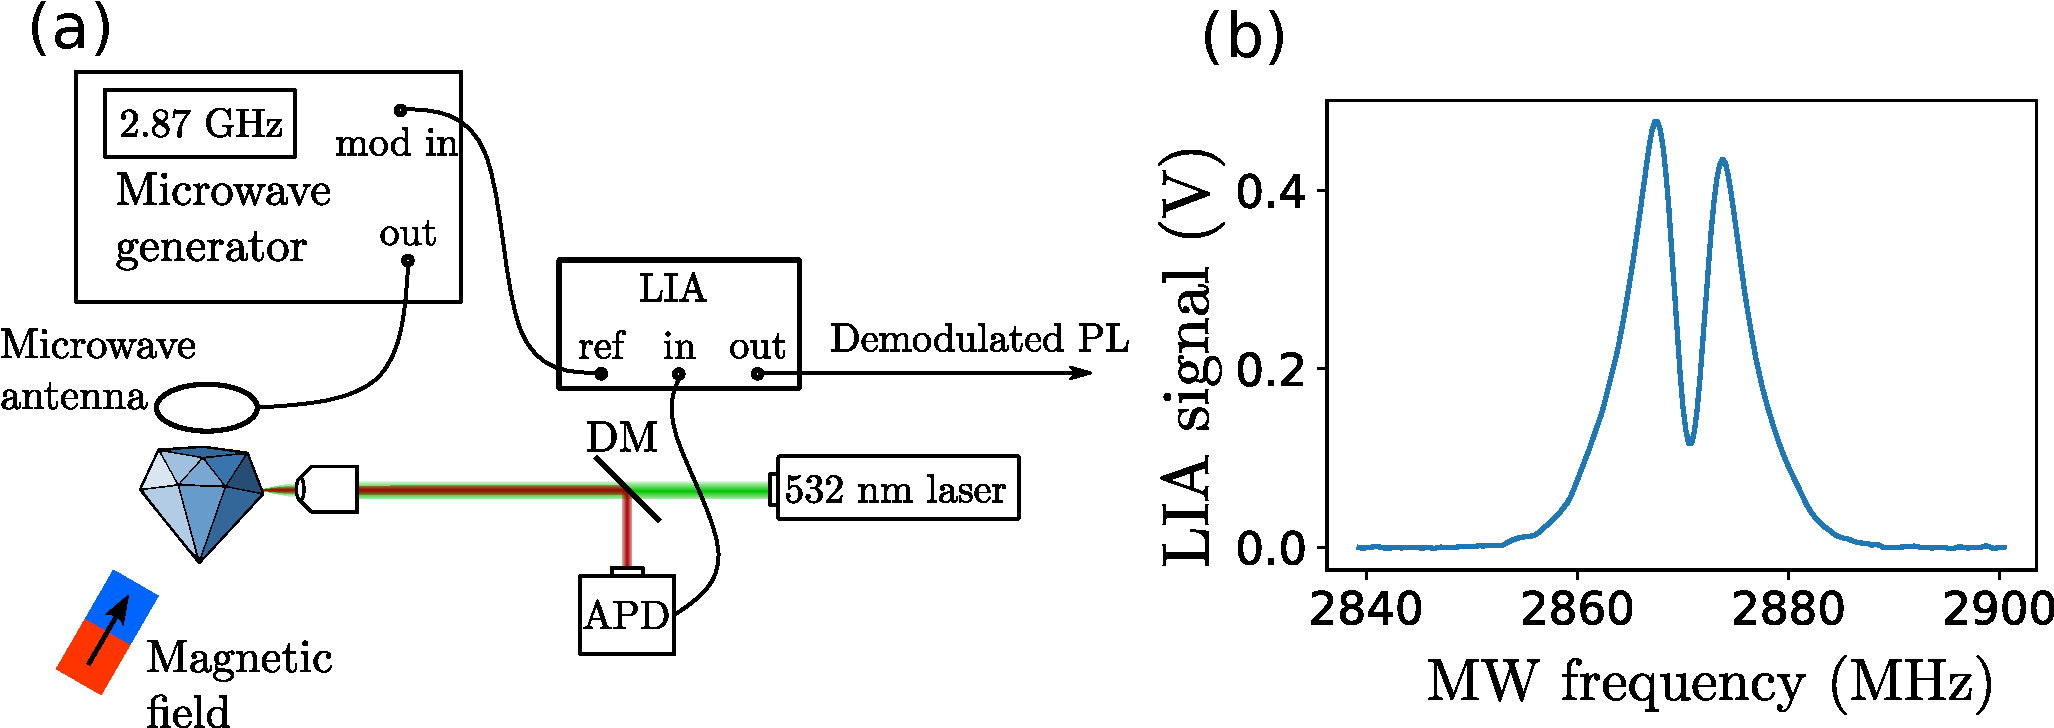
\includegraphics[width=\textwidth]{chapter 1/Figures/ODMR_lockin}
\caption{ODMR protocol with lock-in detection. (a) Simplified confocal microscope setup with a lock-in amplifier (LIA) modulating the mircowave and demodulating the PL. (b) Demodulated ODMR spectrum with no magnetic field on sample ADM-15-4 (see sample details in appendix \ref{Appendix samples}).}
\label{ODMR lockin}
\end{figure}

The ODMR protocol is well suited for lock-in detection with a modulation of the microwave amplitude or frequency modulation \footnote{These are preferred to laser modulation as only the spin part of the NV centers is affected by the microwave field}.

The principle of lock-in detection will not be covered here, the key idea is that lock-in detection allows to translate the signal spectrally in a region less prone to noise. In this case, the ODMR signal is a DC measurement and is therefore prone to slow freqency noise such as electric noise, thermal or mechanical drifts and laser amplitude fluctuations. The microwave field can thus be modulated (in amplitude, frequency or phase) at a frequency fast enough to mitigate the low frequency noise, but slow enough compared to the NV photodynamics. 

Fig. \ref{ODMR lockin}-a) shows the ODMR lock-in setup, and Fig. \ref{ODMR lockin}-b) shows an example of ODMR spectrum with microwave amplitude modulation. All the lock-in spectra shown in this manuscript were produced with 100 \% amplitude modulation at a frequency $f_{\rm mod} \sim 1\ \rm kHz$.

\subsection{ODMR with NV ensemble: longitudinal and transverse magnetic field}
\label{sec champs transverse}
\begin{figure}[h!]
\centering
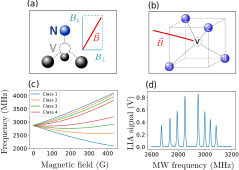
\includegraphics[width=\textwidth]{chapter 1/Figures/ODMR_8_classes}
\caption{(a) Geometry of the NV center and definition of $B_z$ and $B_\perp$. (b) Representation of the 4 possibles orientations (``classes") of the N$-$V axes, corresponding to the 4 $\langle 111 \rangle$ directions of the diamond cubic cell. (c) Simulation of the evolution of the transition frequencies for each class of NV centers as a function of the amplitude of the applied magnetic field ($\textbf{B}$ orientation chosen arbitrarily). (d) ODMR spectrum on sample ADM-150-1 (see sample details in appendix \ref{Appendix samples}) for a magnetic field of $\sim 90\ \rm G$.}
\label{ODMR 8 classes}
\end{figure}

We mentioned previously that the NV spin Hamiltonian (eq. (\ref{NV spin Hamiltonian basic})) was anisotropic due to the fine structure term $D S_z^2$ where $z$ is the direction of the N$-$V axis in the crystal. The magnetic field is thus often decomposed as a sum of a longitudinal magnetic field $B_z$ and a transverse magnetic field $B_\perp=\sqrt{B_x^2+B_y^2}$ (see Fig. \ref{ODMR 8 classes}-a). 

For weak magnetic fields ($\gamma |\textbf{B}| \ll D$), the energy of each of the three spin Hamiltonian eigenstates $\ket{0}$, $\ket{+1}$ and $\ket{-1}$\footnote{The notation $\ket{0}$, $\ket{\pm 1}$ to designate the spin Hamiltonian eigenstates is slightly abusive as $S_z$ does not commute with $\mathcal{H}$ when $B_\perp \neq 0$. The true eigenstates however remain close to $\ket{0}$, $\ket{\pm 1}$ as long as $\gamma_e B_z > \frac{(\gamma_e B_\perp)^2}{D}$.} can be approximated in a perturbative approach by: %cf AN.py
\begin{align}
\nu_0&= -\frac{(\gamma_e B_\perp)^2}{D}, \nonumber \\
\nu_{-1} &= D - \gamma_e B_z + \frac{(\gamma_e B_\perp)^2}{2D}, \nonumber \\
\nu_{+1} &= D + \gamma_e B_z + \frac{(\gamma_e B_\perp)^2}{2D}.
\end{align}

Fig. \ref{ODMR 8 classes}-b) represent the 4 possible orientation of the N$-$V axis in a diamond single crystal. We refer to these orientations as ``classes" since NV centers belonging to the same class will perceive the same transverse and longitudinal magnetic field, and thus will have the same spin Hamiltonian. For large NV ensembles (a confocal spot can contain more than $10^9$ NV centers in dense ensemble), we can consider that each class is equally represented \footnote{It is possible to create NV centers with a preferential orientation \citep{lesik2014perfect} but this requires specific conditions during the growth process of the diamond.} and that each class gives rise to two lines in the ODMR spectrum (one for the $\ket{0} \to \ket{-1}$ transition and one for the $\ket{0} \to \ket{+1}$ transition). 

Fig. \ref{ODMR 8 classes}-c) shows a simulation of the evolution of the transition frequencies $\nu_{+1} - \nu_{0}$ and $\nu_{-1} - \nu_{0}$ for all 4 classes as a function of the magnetic field amplitude, the magnetic field orientation being held to an arbitrary direction. Fig. \ref{ODMR 8 classes}-d) shows an ODMR spectrum with NV ensembles. 8 lines are visible corresponding to the two transitions of the 4 classes. From the position of these 8 lines, it is possible to determine the projection of the magnetic field on each of the 4 N$-$V axes, and thus to reconstruct the full 3D magnetic field with respect to the diamond crystalline axes.

We should also note that the state mixing caused by the transverse magnetic field deteriorates the polarization scheme detailed in Sec. \ref{sec ISC}. For strong transverse magnetic fields ($\gamma_e B_\perp \sim D$), the optical polarization is almost completely quenched, which prevents any kind of coherent NV manipulation \citep{tetienne2012magnetic}.

\section{Dynamics of the NV center spin}

This section focuses on the dynamics of the NV spin, and more specifically on its various relaxation times. Relaxation times are important properties of spin qubits as they often are the limiting factor for quantum information or quantum sensing applications \citep{de2021materials, degen2017quantum}.

There are different relaxation times corresponding to different physical aspects. The longitudinal relaxation time $T_1$ corresponds to the characteristic time of the return to thermal equilibrium for the populations (diagonal elements of the density matrix). The transverse relaxation times $T_2$ and $T_2^*$ correspond to the relaxation of the coherences  (off-diagonal terms of the density matrix).

$T_2$ and $T_2^*$ are called the homogeneous and inhomogeneous dephasing times\footnote{We follow here the NMR nomenclature.}. $T_2^*$ represents to the absolute dephasing time of the spin (or spin ensemble) coherence, while $T_2$ represent the dephasing time measured when a dynamical decoupling scheme is used (Hahn echo \citep{hahn1950spin}, XY-n \citep{maudsley1986modified}, CPMG \citep{carr1954effects} , ...). While the $T_2^*$ value is absolute, the $T_2$ value depend on the precise decoupling scheme used. $T_2$ and $T_2^*$ values are ultimately limited by the spin lifetime:
\begin{equation}
T_2^* < T_2 < 2 T_1.
\end{equation}

The relaxation times of NV centers depend mainly on their environment, and can vary by several order of magnitude depending on the employed sample. The following paragraphs will present the measurement protocols of the different relaxation times and the typical values for the samples used in this manuscript.

\subsection{NV spin $T_1$}
\label{sec T1 NV}
\subsubsection{Measurement protocol}
\begin{figure}[h!]
\centering
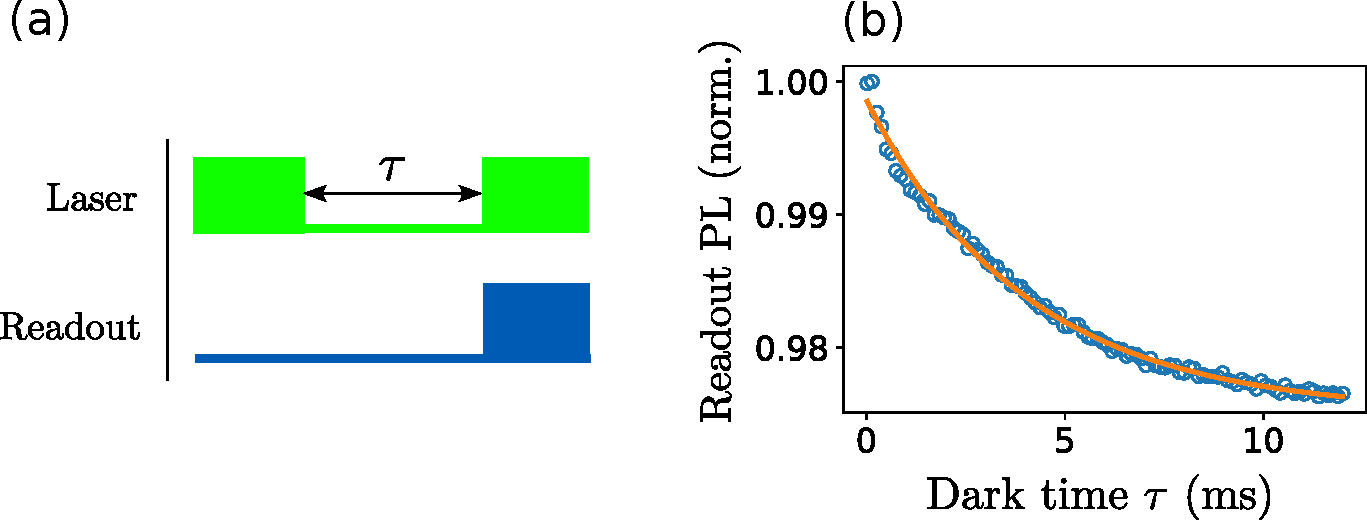
\includegraphics[width=\textwidth]{chapter 1/Figures/T1_basique}
\caption{Basic $T_1$ measurement scheme. (a) Pulse seqeunce used. (b) Experimental data obtained on sample CVD-pink (see sample details in appendix \ref{Appendix samples}.) for low laser intensity. The orange line corresponds to an exponential fit with time constant $\tau=4.0\ \rm ms$.}
\label{T1 basique}
\end{figure}

Fig. \ref{T1 basique} shows a basic protocol to measure the NV $T_1$ time. Fig. \ref{T1 basique}-a) shows the pulse sequence used, which in this case does not involve a microwave field, and Fig. \ref{T1 basique}-b) shows the measured PL obtained by varying the dark time $\tau$. The curve can then be fitted to obtain the spin ensemble $T_1$ value.

\begin{figure}[h!]
\centering
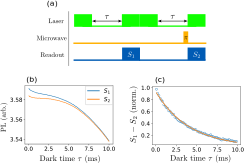
\includegraphics[width=\textwidth]{chapter 1/Figures/T1_protocole_soustraction}
\caption{Common mode rejection $T_1$ measurement scheme. (a) Pulse sequence. (b) PL signals $S_1$ and $S_2$ obtained on sample CVD-pink with a high laser intensity ($I_{\rm las}=5\ \rm mW$). (c) Subtraction $S_1-S_2$ versus dark time $\tau$. The experimental data is fitted with an exponential decay of time constant $\tau=4.1\ \rm ms$.}
\label{T1 soustraction}
\end{figure}

The sequence shown in Fig.\ref{T1 basique} can be improved by implementing a common mode rejection technique described in Fig. \ref{T1 soustraction}-a). This protocol works as follow: first, a basic $T_1$ sequence is recorded, which we will denote $S_1$. Then the sequence is repeated with the addition of a $\pi$-pulse on one the NV transitions right before the readout. This $\pi$-pulse inverts the population of the $\ket{0}$ and $\ket{\pm 1}$ states. The second readout is labeled $S_2$, and the final spin state readout is $S_1 -S_2$ which rejects every contribution to the PL besides the spin relaxation. 

Fig. \ref{T1 soustraction}-b) shows the experimental result of the $S_1$ and $S_2$ sequences on the same sample that was used in Fig. \ref{T1 basique}, with a higher laser intensity. We can notice a stark difference between the $S_1$ curve in Fig. \ref{T1 soustraction}-b) and the curve in Fig. \ref{T1 basique}-b), despite both of them coming from the same sample and with the same measurement protocol. The reason for the difference is that the higher laser intensity used in Fig. \ref{T1 soustraction} photoionizes some of the $NV^-$ into NV$^0$ via a two-photon absorption scheme. The NV$^0$ can then capture an electron during the dark time \citep{giri2018coupled, giri2019selective} which changes the number of NV$^-$ centers probed depending on the dark time length. The goal of the subtraction scheme is to suppress this charge state recombination noise which is common to the two sequences $S_1$ and $S_2$.

Fig. \ref{T1 soustraction}-c) shows the subtraction of the $S_1$ and $S_2$ signal. Despite the complex shape of the initial $S_1$ and $S_2$ signals, $S_1-S_2$ is satisfyingly fitted by an exponential decay similar to the results found in Fig. \ref{T1 basique}.

The photodynamics of the NV charge state is a complex subject which is still actively researched \citep{craik2020microwave, gorrini2021long}. The common mode rejection scheme described  here is often employed with dense ensemble of NV centers \citep{jarmola2012temperature, mrozek2015longitudinal, choi2017depolarization} as it allows to completely bypass the charge dynamics.

\subsubsection{Physical origin and typical values}

We distinguish three different origin for the the $T_1$ relaxation process:
\begin{itemize}
\item \textbf{Spin-phonon relaxation:} the spin states are weakly coupled to the crystal phonon bath through spin-spin and spin-orbit interactions \citep{norambuena2018spin}, which can result in a phonon-induced spin relaxation. The dominant relaxation mechanism depends on the  temperature regime, with the two-photon Raman process believed to be dominant at room temperature \citep{takahashi2008quenching, jarmola2012temperature} while the dominant process as at cryogenic temperature ($4\sim100$ K) is believed to be a two phonons Orbach process \citep{redman1991spin, norambuena2018spin}. The spin-phonon relaxation time strongly depends on the crystal lattice temperature, with relaxation times of the order $T_1 \sim 5\ \rm ms$ at room temperature, and up to 8 hours at  mK temperatures \citep{astner2018solid}.

\item \textbf{Electric and magnetic field noise:} both electric and magnetic fields can directly excite the $\ket{0} \to \ket{\pm 1}$ spin transition \citep{udvarhelyi2018spin}. As a result, magnetic and electric field noise can reduce the spin $T_1$ if a significant portion of their power spectral density overlaps with the NV spin transitions. This is particularly important for near surface spins because of the strong noise caused by electronic defects on the surface \citep{sangtawesin2019origins}. The $T_1$ of near surface NV center can be as low as $\sim 10\ \mu$s, but the surface effects are only effective at very short range (within $\sim 10\ \rm nm$ of the surface).

\item \textbf{Resonant dipolar interaction with other paramagnetic impurities:} Dipole-dipole interaction between NV centers and surrounding spins is responsible for both transverse and longitudinal spin relaxation, with the added condition of energy matching (resonance) for longitudinal relaxation. The $T_1$ time associated with dipole-dipole interaction strongly depends on the spin concentration.
\end{itemize}

All the measurements shown in this manuscript were performed at room temperature. The spin-phonon interaction thus creates a baseline value for the NV $T_1$ time at $\sim 5\ \rm ms$. Every sample studied were at least a few $\mu$m thick and we will therefore neglect the surface noise contribution in our analyses. The dipole-dipole induced relaxation however is of crucial importance for the next chapters, where it will be further detailed. $T_1$ times between $0.1 \sim 1\ \rm ms$ were routinely observed for samples with high NV concentration.

\subsection{NV spin $T_2^*$}
\subsubsection{Measurement protocol}
\begin{figure}[h!]
\centering
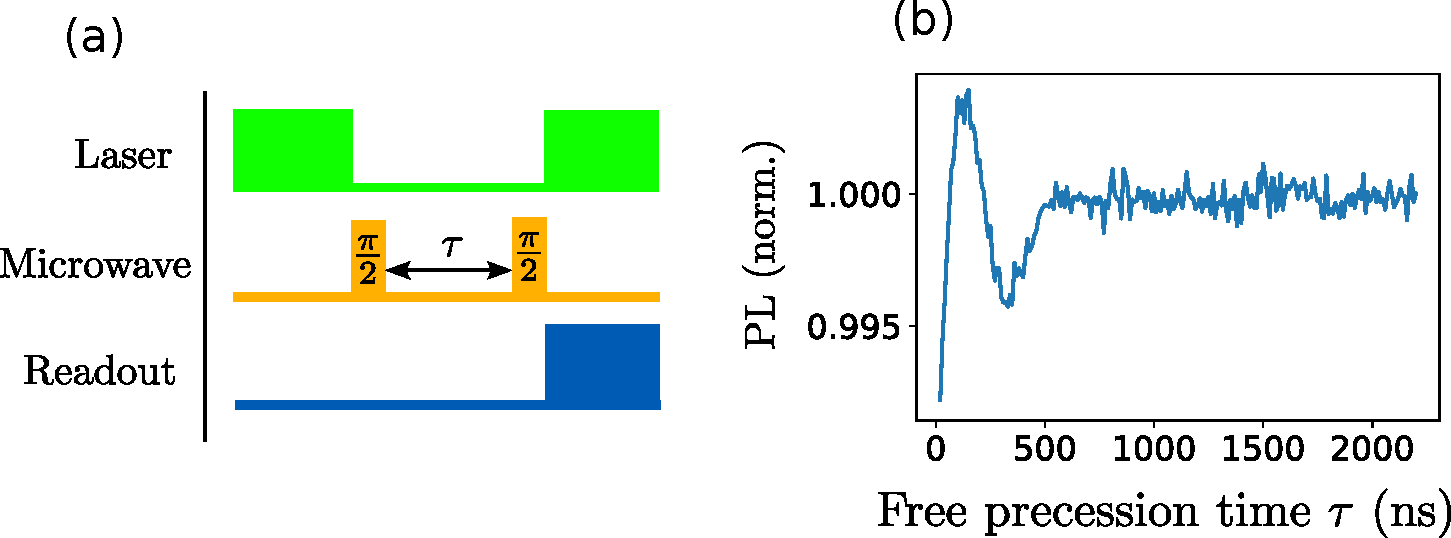
\includegraphics[width=\textwidth]{chapter 1/Figures/Ramsey}
\caption{Ramsey interferometry protocol. (a) Pulse seqeunce used. (b) Experimental data obtained on sample CVD-pink.} %The orange line corresponds to an Gaussian fit with time constant $\tau=400 \pm 100\ \rm ns$.}
\label{Ramsey}
\end{figure}

$T_2^*$ is the characteristic timescale of the loss of quantum coherence for a freely evolving system. It is generally defined as the decay time in a Ramsey interferometry measurement \citep{barry2020sensitivity}.

Fig. \ref{Ramsey}-a) shows the Ramsey pulse sequence: after being initialized in the $\ket{0}$ state, the NV spin is transformed with a $\pi/2$ pulse in a coherent superposition of $\ket{0}$ and $\ket{\pm 1}$ which freely precesses at the Larmor frequency. After a free precession time $\tau$, the remaining coherence is projected back into spin population with a second $\pi/2$ pulse. Fig. \ref{Ramsey}-b) shows an experimental example obtained on a spin ensemble. The microwave frequency is detuned by $\sim 300\ \rm kHz$ with respect to the spin central Larmor frequency which causes oscillations in the signal. $T_2^*$ is the decay time of the envelope of the Ramsey fringes. It is unfortunately difficult to correctly fit the envelope of a signal with so few fringes, a recurring issue with our current microwave setup. 

Ramsey sequences are generally harder to perform on NV ensemble than they are on single NV for two main reasons. The first one is that the $T_2^*$ times tend to be longer for single NV centers as they do not suffer from spatial inhomogeneity, and because the samples used for single NV experiments generally contains less impurities than those used for NV ensemble. The second one is the inhomogeneous microwave power which leads to a variation of the Rabi frequencies among the spins \citep{barry2016optical, zhou2020quantum} and lowers the fringe contrast.

An alternative measurement of $T_2^*$ can be performed by measuring the linewidth of an ODMR spectrum. Indeed, ideally the ODMR spectrum should be the Fourier transform of the Ramsey signal (also called free induction decay in NMR literature). In practice however, both methods suffer from experimental noise and imperfections, with Ramsey-type methods being more sensitive to microwave inhomogeneities \citep{barry2020sensitivity} while ODMR is prone to laser and microwave power broadening \citep{dreau2011avoiding}. 

The method chosen to extract $T_2^*$ values in this manuscript was ODMR at low microwave power ($\Omega_{\rm Rabi} \ll 1/T_2^*$) and low laser intensity (compared to the NV optical saturation).

\subsubsection{Physical origin}

\begin{figure}[h!]
\centering
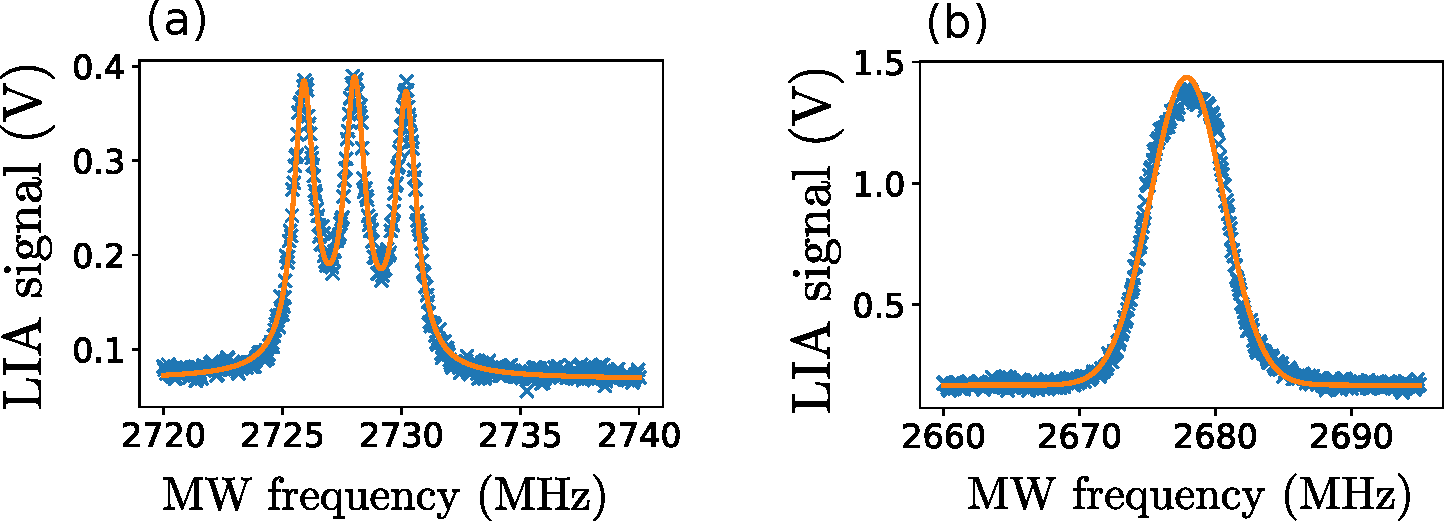
\includegraphics[width=\textwidth]{chapter 1/Figures/ODMR_1_classes}
\caption{ODMR spectra on a single NV class. (a) Experimental data on sample CVD-pink, fitted with three Lorentzians with HWHM $530$ kHz ($T_2^*=300\ \rm ns$). (b) Experimental data on sample Sumi-2, fitted with a single Gaussian with HWHM $3.2$ MHz ($T_2^*=83 ns$).}
\label{ODMR 1 classe}
\end{figure}

For most samples, the leading cause of inhomogeneous dephasing is the temporal and spatial variations of magnetic fields caused by the paramagnetic impurities in the crystal \citep{barry2020sensitivity}. The nature of these different paramagnetic impurities will be further discussed in the section dedicated to dark spins in diamond in chapter 2. We will simply mention here that for sample with high NV density ([NV] $\geq$ ppm), $T_2^*$ is mostly limited by the electronic spins of nitrogen impurities \citep{bauch2018ultralong}.

Fig. \ref{ODMR 1 classe} shows ODMR spectra of a single NV class on two distinct samples (see sample details in appendix \ref{Appendix samples}). The first sample is a CVD sample with a total substitutional nitrogen  concentration $[N_s] \approx 26\ \rm ppm$, while the second is a type-Ib HPHT sample with a likely nitrogen concentration $[N_s] \geq 100\ \rm ppm$. We can clearly see a higher linewidth, corresponding to a smaller $T_2^*$ value on the sample with higher nitrogen concentration. In particular, we can notice the hyperfine structure of the $^{14}$N nuclei on the CVD sample, whereas it is hidden by the inhomogeneous broadening on the HPHT sample.

Fig. \ref{ODMR 1 classe} illustrates another difficulty of $T_2^*$ measurement which is to find the correct fitting formula. While the spectral profile of single NV centers is expected to be Gaussian, the spectral profile of an ensemble of NV centers  is expected to be Lorentzian \citep{dobrovitski2008decoherence, hall2014analytic}. For Fig. \ref{ODMR 1 classe}-a), it was indeed found that Lorentzians fitted the data better than Gaussians. For Fig. \ref{ODMR 1 classe}-b) however, a Gaussian was found to be a better fit than a Lorentzian, although this could be in part due to the unresolved hyperfine structure.

\subsection{NV spin $T_2$}
\label{sec T2 echo}
\begin{figure}[h!]
\centering
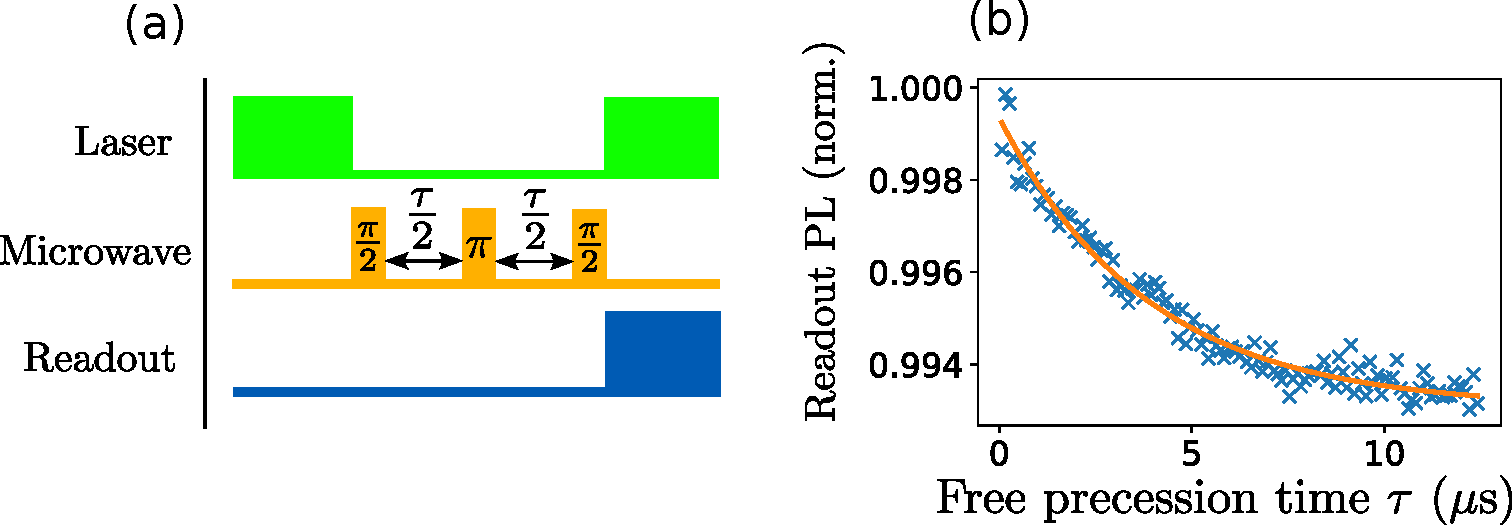
\includegraphics[width=\textwidth]{chapter 1/Figures/Echo}
\caption{Spin-echo protocol. (a) Pulse seqeunce used. (b) Experimental data obtained on sample CVD-pink, fitted with an exponential decay of time $3.9\ \rm{\mu s}$.} 
\label{Echo}
\end{figure}
\subsubsection{Measurement protocol}
As precised earlier, the exact $T_2$ definition depends on the rephasing scheme used. We will focus here on the simplest known rephasing process which is the spin-echo or Hahn-echo sequence.

Fig. \ref{Echo} shows the pulse sequence used and an example on the same sample than the Ramsey measurement. The pulse sequence differs from the Ramsey one by adding a a $\pi$-pulse in the middle of the free precession time. This additional $\pi$-pulse causes static or slowly varying dephasing to be rephased \citep{hahn1950spin}. 

This protocol extends the coherence time on this particular sample from $T_2^* \approx 300\ \rm ns$ to $T_2 \approx 4\ \rm{\mu s}$, an increase by more than a factor of 10. Improvement by a factor of $10 \sim 100$ or typical for NV ensembles \citep{barry2020sensitivity}. This value could likely be extended even further by using a more complex dynamical decoupling scheme from the CPMG or XY sequence families \citep{naydenov2011dynamical, bar2012suppression}.

\subsubsection{Physical origin}
The origin of the relaxation time $T_2$ are fluctuating noises which are too fast to be efficiently rephased by the sequence. The origin of these noises is generally attributed to the flipping of spins in the vicinity of the NV center (either through spin-lattice or spin-spin mechanisms) \citep{hall2014analytic}. For samples with high nitrogen concentration, it has been measured that the $T_2$ time  was directly correlated to the nitrogen concentration, with the same scaling than the $T_2^*$ time \citep{bauch2019decoherence}.

\section{Conclusion}

We have covered in this introductory chapter every concepts needed to understand the results presented in the next chapters. We have seen the main steps in the creation of artificial diamonds and NV centers, we have covered the optical and spin properties of the NV center as well as the ways to measure them, and we have introduced the notion of dipole-dipole coupling and cross-relaxation between two spins.

The focus of chapter 2 will be on the cross-relaxation between NV centers and other spin impurities in CVD-grown diamond, while the focus of chapter 3 and 4 will be on the cross-relaxation between NV centers and other NV centers, as well as their potential application in magnetometry.

\chapter{Cross-relaxations between NV centers and dark spins in CVD-grown diamond}
Crystal defects are promising candidates for quantum information technologies, either through their optical or spin degree of freedom \citep{aharonovich2016solid, atature2018material, bassett2019quantum}. Spectrocopic studies are a necessary step in identifying and characterizing these defects, with electron paramagnetic resonance (EPR) being the spectrocopic tool of choice to measure the spin properties of the defects \citep{newton2007epr}. 

In this chapter, we present a method to characterize the spin of diamond impurities through cross-relaxation with NV centers \citep{hall2016detection,pellet2021optical}. This method allows an all-optical detection of non-NV center spin defects, a method that is both cheaper and more sensitive than traditional EPR. We focus in particular on defects in CVD-grown diamonds which have historically been less studied than HPHT diamond, and for which no prior NV cross-relaxation had been reported. 

The chapter is organized as follow: we will first detail the most common paramagnetic impurities in the diamond (the so-called ``dark spins") before explaining the proceeding of NV cross-relaxation experiments, and more generally of NV relaxometry. We will then focus on the detection of two particular defects in a CVD diamond, VH$^-$ and War1, and on their characterization (density, spin parameters, temperature dependence). We will finally conclude on the possible improvements and application of this detection method.

The work presented in this chapter has been published in large part in the articles \citep{pellet2021optical, ngambou2022improving}.


\section{Dark spins in diamond}

\begin{figure}[h!]
\centering
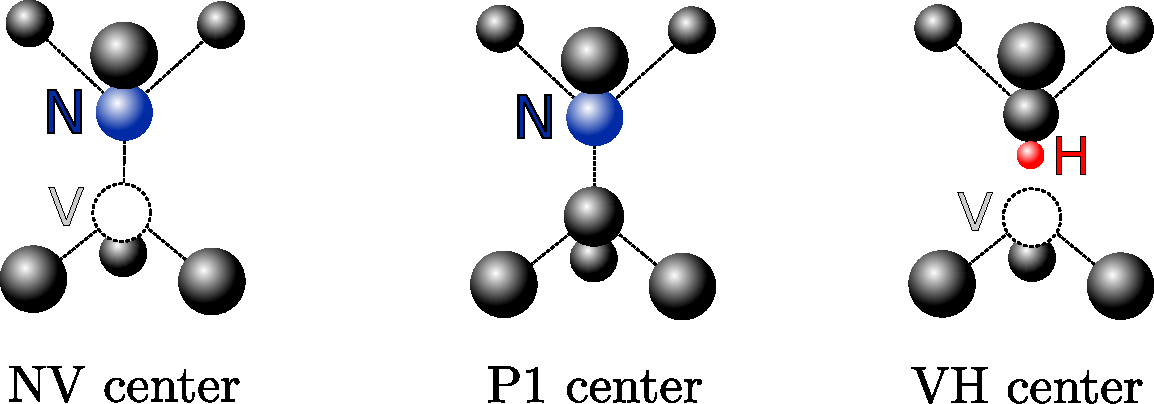
\includegraphics[width=.7\textwidth]{chapter 2/Figures/tronche_de_spin}
\caption{Crystalline structure of three spin defects: the NV center, the P1 enter (substituional Nitrogen) and the VH center.} 
\label{repr NV P1 VH}
\end{figure}

We refer by dark spins to paramagnetic impurities for which the spin degree of freedom is not accessible optically. At room temperature, only two defects in diamond do not have a dark spin: the NV center and the more recently found ST1 center \citep{lee2013readout, john2017bright}. Every other spin impurity identified so far is considered to be dark.

In this section we will present the most common dark spins encountered in diamond, which are simply the most common paramagnetic impurities aside from the NV center, and the relation between the diamond growth process and the presence of these impurities. We will also briefly present EPR spectroscopy which is the most common method to characterize these dark spins.

\subsection{P1 centers and $^{13}$C}
The most common spin defects in NV-rich diamond are the substitutional nitrogen centers N$^0_S$ known as the P1 centers (see Fig. \ref{repr NV P1 VH}), which have an electronic spin $1/2$ and a nuclear spin 1, and the $^{13}$C $1/2$ nuclear spin which represents 1.1\% of natural abundance carbon atoms, the remaining carbon atoms being almost exclusively the spinless $^{12}$C isotope. In NV-rich diamonds, these two impurities are the main causesof the NV center dephasing rates $\Gamma_2^*=1/T_2^*$ and $\Gamma_2=1/T_2$  \citep{barry2020sensitivity}. 

The dephasing rate caused by a given impurity is directly proportional to the average diagonal dipole-dipole matrix elements ($\Omega_{\rm shift}$ in (eq. \ref{eq. ff df})) between the two spin species \citep{taylor2008high, bauch2020decoherence}. Since the dipole-dipole interaction scales as $1/r^3$, and the distance $r$ between each spin scales as the inverse cubic root of the concentration,  it is expected that the dephasing rate associated with a particular impurity scales linearly with the concentration of the impurity: $\Gamma_2^*(\rm P1) \propto [P1]$. 

In the case of P1 centers, this was verified experimentally by looking at controlled sample with varying concentration of nitrogen \citep{bauch2020decoherence}. The authors of the study found a value of $\Gamma_2^*(\rm P1)= (2 \pi) 16\ \rm kHz/ppm$. 

$^{13}$C nuclei are typically much more abundant than P1 center ($\sim$ 10 000 ppm without istopic engineering) but being a nuclear spin, it has a gyromagnetic ratio $\approx 2.8\cdot 10^3$ times smaller than that of the P1. As a result, the contribution of a single $^{13}$C nucleus to the NV dephasing rate is $\sim 10^3$ times that of a single P1 center. It was found experimentally that the broadening caused by $^{13}$C is $\Gamma_2^*(^{13}\rm C ) \approx (2 \pi) 16\ \rm Hz/ppm$ \citep{van1997dependences, barry2020sensitivity}. In samples with natural isotopic abundance of carbon, the inhomogeneous dephasing rate due to the $^{13}$C nuclear spins has a value $\Gamma_2^*(^{13}\rm C ) \approx (2 \pi) 160\ \rm kHz$.

\subsection{Other spin defects, VH$^-$, War1}
\label{other defects}
Other spin defects are also commonly found in diamond containing NV centers, such as charged vacancy or vacancy clusters \citep{hounsome2006origin}, other nitrogen related defects \citep{newton2007epr}, transition metals \citep{isoya1990fourier}, and especially for CVD grown diamond, hydrogen related defects \citep{hartland2014study}, since the CVD plasma contains up to 95 \% hydrogen (see sec. \ref{fab HPHT}).

Of particular interest in this chapter are two defects: the VH$^-$ defect \citep{glover2003hydrogen, glover2004hydrogen} and the War1 defect \citep{cruddace2007magnetic}. 

The VH$^-$ defect, prior to our observations, had only been observed via electron paramagnetic resonance (EPR) in CVD grown diamond. It is formed by a vacancy with a hydrogen atom forming a bond with one of the four neighboring carbon atoms (see Fig. \ref{repr NV P1 VH}). To acquire its negtatively charged state, the VH center needs to capture an electron from a donor in the crystal, similarly to the NV center. 

This defect has a similar electronic structure as the NV$^-$ which results in an electronic spin-1 with a similar zero field splitting parameter (see Table \ref{table VH et War1}). Although the presence of hydrogen in this defect was confirmed by isotopic study, it has been debated whether this defect was VH$^-$ or V$_2$H$^-$ due to a conflict with \textit{ab initio} calculations \citep{shaw2005importance}. The defect is therefore sometimes referred to as V$_n$H$^-$. In this manuscript we will employ the original terminology: VH$^-$.

The War1 defect, named after the University of Warwick where it was first observed in a CVD diamond \citep{cruddace2007magnetic}, is another spin-1 defect whose chemical structure remains unknown. No hyperfine structure could be discerned in the relatively broad EPR line, and the use of deuterium instead of $^1$H did not change the shape of the line.

\subsection{EPR spectroscopy}
\begin{figure}[h!]
\centering
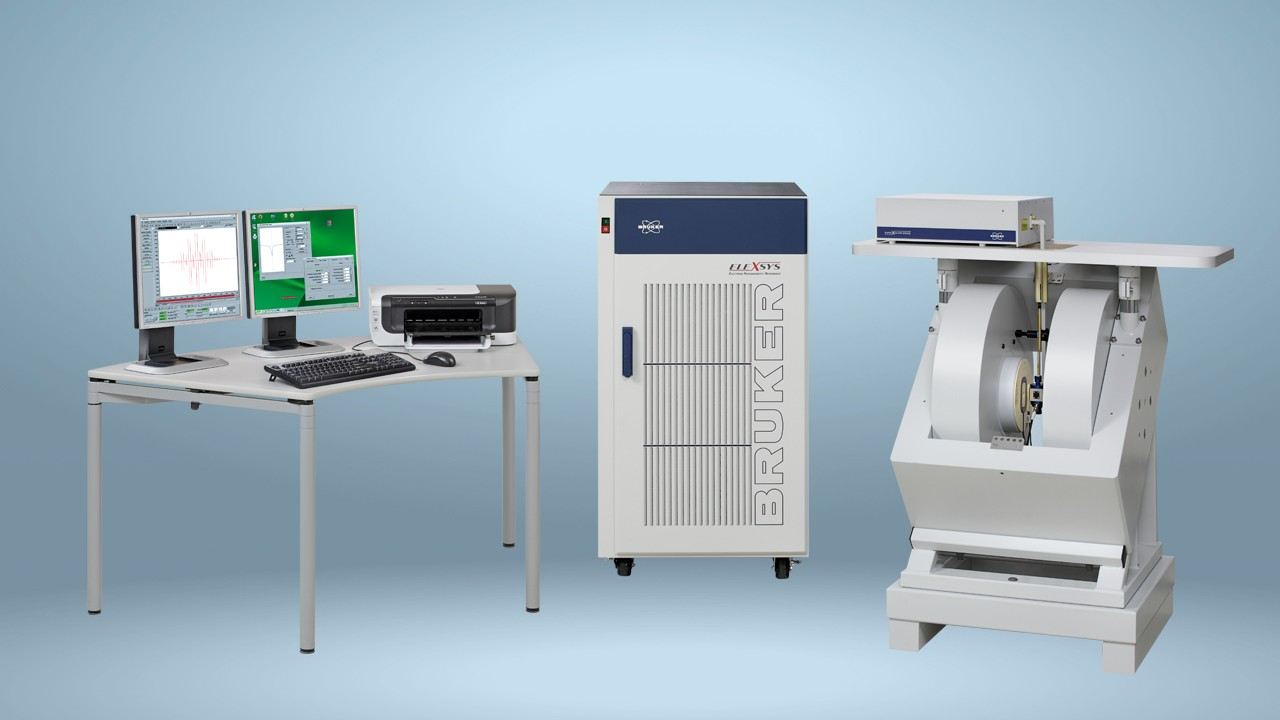
\includegraphics[width=.7\textwidth]{chapter 2/Figures/EPR_spectometer.jpg}
\caption{EPR specrometer. Credits: Bruker Corporation} 
\label{photo EPR}
\end{figure}

Electron paramagnetic resonance (EPR), the electronic equivalent to NMR, is the the most common way to detect electronic spins in solids and liquids. The principle of its detection is the absorption or reflection of a microwave field resonant with a spin transition.

EPR generally relies on the thermal polarization of the spins to observe an absorption. In order to increase the polarization, an important magnetic field is applied (typ. 0.35 T or 3500 G) and a microwave cavity (typ. 9500 MHz) is used to improve the coupling of the spins to the field.

The usual EPR apparatus, shown in Fig. \ref{photo EPR}, is a bulky and expensive lab equipment ($\gtrsim$ 1 M€). In contrast, optical detection such as ODMR is technically easier, less expensive, and allows better spatial resolution. 

ODMR can also be significantly more sensitive than EPR: single NV centers are routinely observed in ODMR while the the current EPR noise floor for electronic spins in diamond is typically of $\sim 10^{11}$ spins \citep{mitchell2013x}. This difference in sensitivity comes in part from the better spin polarization \footnote{At room temperature, the thermal polarization of a spin with a transition at 9500 MHz is $\sim 0.002$ while the NV center optical polarization can reach 0.8.}, and in part from the more efficient photon detection in the optical range than in the microwave range.

The key idea of this chapter is to allow the optical detection of spin defects that normally do not show ODMR thanks to cross-relaxation with NV centers.

\section{NV center relaxometry}

Detection of dark spins via NV center cross-relaxation fall under the more general technique of NV relaxometry, which consists in measuring a modification of the NV center spin lifetime $T_1$. Relaxometry with NV centers has been used not only to measure cross-relaxation with dark spins \citep{van1989cross, holliday1989optical, epstein2005anisotropic, armstrong2010nv,   hall2016detection, wickenbrock2016microwave,  wood2016wide,  alfasi2019detection, lazda2021cross}, but also to probe the magnetic noise in the diamond environment coming from spins \citep{steinert2013magnetic}, ions\citep{tetienne2013spin}, free radicals \citep{nie2021quantum}or magnetic domains \citep{finco2021imaging}. 

The protocols used in NV relaxometry measure either directly the spin $T_1$ or indirectly through the NV photoluminescence.

\subsection{PL and single$-\tau$ relaxometry protocols}
\begin{figure}[h]
\centering
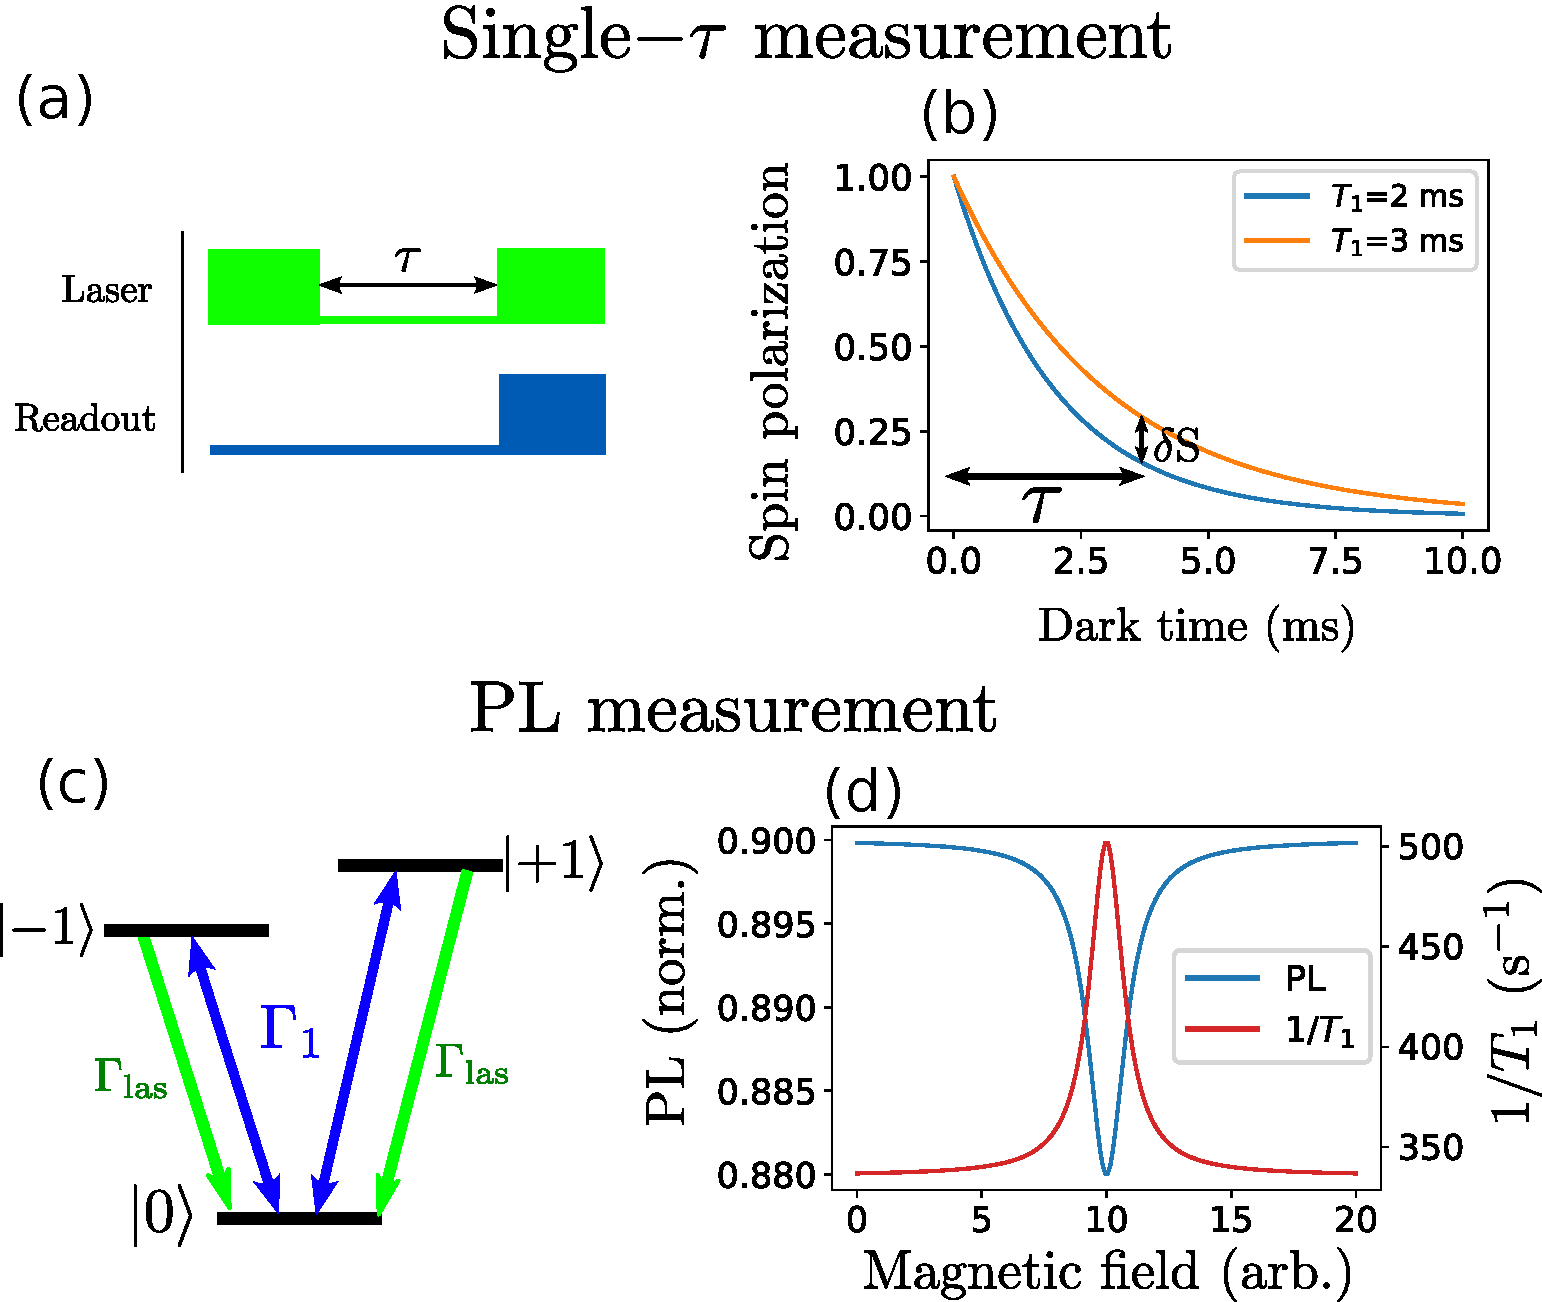
\includegraphics[width=0.9\textwidth]{chapter 2/Figures/relaxo_pulsed_continuous_2}
\caption{Representation of the two relaxometry protocol. (a) Simple $T_1$ measurement pulse sequence. (b) Simulation of two $T_1$ measurement with different $T_1$ values. $\tau$ represents the optimal dark time in order to maximize the signal $\delta S$ (c) Representation of the optical pumping (green arrows) and depolarization (blue arrows) of the NV center spin. (d) Simulation of the PL modification caused by a change in the spin $T_1$. The spin $T_1$ profile in term of the magnetic field was arbitrarily chosen.}
\label{T1 vs PL}
\end{figure}

The two most common NV relaxometry protocols are represented on Fig. \ref{T1 vs PL}. The first method simply consists in measuring the spin lifetime, following the protocols described in \ref{sec T1 NV}. In Fig. \ref{T1 vs PL}, we picture the simpler $T_1$ measurement protocol, but the technique can be used with the common mode rejection protocol. In order to more efficiently measure a modification of the spin $T_1$, the ``single$-\tau$" protocol does not record the entire depolarization curve represented in Fig. \ref{T1 vs PL}-b), but instead probes the spins for a single dark time value $\tau$ \citep{pelliccione2014two, schmid2015relaxometry, tetienne2016scanning}. This value is chosen in order to maximize the change in signal $\delta S$ for a given change in lifetime $\delta T_1$, typically $\tau \sim T_1$.

 The second method simply consists in monitoring the PL of the NV centers : since the PL is proportional to the population in the $\ket{0}$ state, and since the steady state population in the $\ket{0}$ state results from the equilibrium between the optical polarization rate $\Gamma_{\rm las}$ and the depolarization rate $\Gamma_1=1/T_1$. A simple rate equation for the $\ket{0}$ state population $\rho_{00}$ gives:
 \begin{equation}
 \rho_{00}=\frac{\Gamma_{\rm las}+\Gamma_1}{\Gamma_{\rm las}+3\Gamma_1}.
 \end{equation}
 
 Fig. \ref{T1 vs PL} shows a simulation of NV centers PL when the spin decay rate $\Gamma_1$ is modified. In this fictional scenario, we assume that $\Gamma_1$ resonantly increases for a given value of the magnetic field (we will see later in this manuscript physical examples corresponding to this scenario). We can see that the PL decreases as an answer to the $\Gamma_1$ increase. The exact value of the PL drop ($\sim 2\%$ in the crase presented here) depends on the optical polarization rate $\Gamma_{\rm las}$ as well as the modification of the spin lifetime. 

It is argued in \citep{finco2021imaging} that both methods result in similar signal to noise ratio: in the PL case, the laser intensity needs to be adjusted so that $\Gamma_{\rm las} \sim \Gamma_1$ in order to maximize the PL contrast, while the single$-\tau$ method requires a waiting time $\tau \sim T_1$ between each measurement, which results in a similar PL count and shot noise limit in both case.

On a technical level, the PL-based method is easier to implement since it does not require the use of a pulsed laser, and because it requires a smaller laser power to work optimally. It is however more sensitive to drifts and changes in the optical setup. Most of the relaxometry measurement in this manuscript were performed using a PL-based detection.

\subsection{Comparison with DEER protocol}

\begin{figure}[h]
\centering
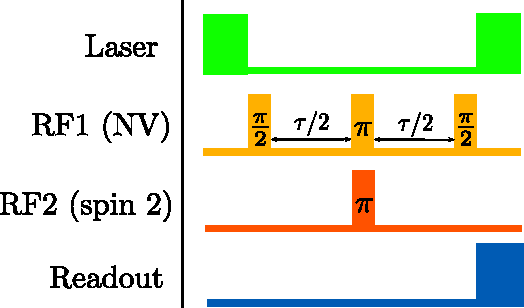
\includegraphics[width=0.5\textwidth]{chapter 2/Figures/DEER}
\caption{Pulse sequence of the DEER protocol}
\label{DEER}
\end{figure}

Aside from cross-relaxations, another protocol exists to address dark spin resonance with NV centers, based on a modification of the NV $T_2$ time \citep{mamin2012detecting, serbyn2014interferometric}. This protocol, called double electron-electron resonance (DEER), is depicted on Fig. \ref{DEER}. The pulse sequence consists in applying a spin-echo on the NV center, as described in \ref{sec T2 echo}, with a simultaneous $\pi-$pulse on the probed dark spins during the rephasing pulse on the NV centers. This additional pulse means that the static (or slowly variable) contribution of the probed spins to the $T_2^*$ of the NV center will not be rephased. The newly measured $T_2$ time should thus be slightly shorter.

\begin{equation}
\frac{1}{T_2^{\rm DEER}}=\frac{1}{T_2^{\rm echo}} + \delta \Gamma_2^*,
\end{equation}

where $\delta \Gamma_2^*$ is the contribution of the dark spin to the $T_2^*$ of the NV center.

By scanning the frequency of the second microwave (RF2) and monitoring the $T_2$ time of the NV centers, one can find dark spin resonance without having to bring them to resonance with NV centers, which can be useful when the dark spin resonance is very far detuned from the NV one.

Both relaxometry and DEER protocols have their own advantages. While DEER allows more control on the probed impurity, allowing in particular coherent control of the dark spin \citep{sushkov2014magnetic}, relaxometry protocols are generally easier to implement as they do not require a pulsed microwave setup. In some cases at least, relaxometry protocols have been shown to be more sensitive than $T_2$ based protocols such as DEER due to the fact that $T_1$ is typically orders of magnitude greater than $T_2$ \citep{steinert2013magnetic}.

Relaxometry protocols do require however specific magnetic field values in order to bring in and out of resonance the two spins involved in the cross-relaxation. The choice of the field orientation and strength in order to best observe NV-dark spin cross-relaxations will be covered in the following section.

\section{Choice of the magnetic field orientation}

As relaxometry does not rely on a microwave field, the only external parameter left to tune is the magnetic field. Typically, the magnetic field is scanned in a fixed direction while the signal, either PL or T1, is recorded. Due to the strong NV anisotropy however, the direction along which $\mathbf{B}$ is scanned plays a crucial role in the ability to detect NV-dark spins CR.

This section focuses on particular field orientation with respect to the diamond crystalline axes, and details the advantages and disadvantages of the two main choices that are the [100] and [111] direction in order to detect four particular dark spins: P1 centers, Vh$^-$, War1 and the $^{13}$C$-$NV complex\footnote{The $^{13}$C$-$NV complex is normally not dark, as will be discussed in its own section.}.

\subsection{The [100] and [111] magnetic field orientations}
\label{sec simu}

\begin{figure}[h]
\centering
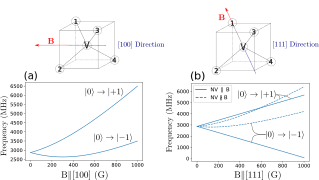
\includegraphics[width=1\textwidth]{chapter 2/Figures/121_vs_22_NV}
\caption{Simulated transition frequencies of the $\ket{0} \to {-1}$ and $\ket{0} \to {+1}$ transitions for the 4 classes of NV centers as a function of the magnetic field. a) When the magnetic field is along the diamond [100] crystalline axis, b) along the [111] axis. A representation of the 4 classes of NV centers, labeled 1 to 4, and the orientation of the magnetic field in both cases is put on top}
\label{121 vs 22 NV}
\end{figure}

Fig. \ref{121 vs 22 NV} shows the two main choices of scanning orientation : either $\mathbf{B} \parallel [100]$ or 
$\mathbf{B} \parallel [111]$ where [100] and [111] refer to the diamond crystalline axes. When $\mathbf{B} \parallel [100]$, all four classes (the different possible NV orientations represented at the top of the figure) are equivalent, whereas for $\mathbf{B} \parallel [111]$, one class is perfectly aligned with the magnetic field while the three others are equivalently unaligned. 

These changes in the field orientation result in important changes in the NV behavior, mainly due to the transverse magnetic field: Fig. \ref{121 vs 22 NV}-a) shows the transition frequency between the $\ket{0}$ and $\ket{\pm 1}$ states of the ground state spin Hamiltonian (REF chapter 1) - or to be more precise the transitions between the ground state of the spin Hamiltonian and the two excited states - for any of the four classes of NV centers when $\mathbf{B} \parallel [100]$. Notably, there is no transitions frequencies below 2500 MHz. 

On the other hand, Fig. \ref{121 vs 22 NV}-b) shows the transition frequencies when $\mathbf{B} \parallel [111]$, for both the class aligned and the three class misaligned. The three classes behave similarly than the four classes in the $[100]$ case, but the one class aligned with the magnetic field can get its $\ket{0}\to\ket{-1}$ transition arbitrarily small, as long as the magnetic field is perfectly aligned with the NV axis.

We will now compare these two possible field orientation in order to observe cross-relaxation between NV centers and the four previously mentioned dark spin species.

\subsection{CR condition between NV$^-$ and P1}

\begin{figure}[h]
\centering
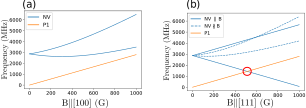
\includegraphics[width=1\textwidth]{chapter 2/Figures/121_vs_22_P1}
\caption{Simulation of the transition frequencies of NV$^-$ centers and P1 centers (without the hyperfine interactions) for a magnetic field a) along the [100] axis and b) along the [111] axis}
\label{121 vs 22 P1}
\end{figure}

P1 centers, the most abundant electronic spin in the diamonds commonly used, have a $1/2$ electronic spin. They do have a small magnetic field anisotropy coming from the hyper-fine coupling to the nitrogen nucleus ($\sim 100\ \rm MHz$), but this dependency on the field orientation is small compared to the NV center's zero field splitting $D=2870\ \rm MHz$. We can therefore, to the first order, neglect the hyper-fine coupling and consider P1 centers as ideal, isotropic, spin $1/2$.

Fig. \ref{121 vs 22 P1} shows the transition frequencies for the NV center and such a spin $1/2$, as a function of a magnetic field parallel to [100] or [111]. When $\mathbf{B} \parallel [100]$, there will never be a co-resonance between the NV and P1 transitions, meaning that no NV-P1 cross-relaxation can be observed when B is scanned in this direction. When $\mathbf{B} \parallel [111]$ however, the P1 $\ket{-1/2} \to \ket{+1/2}$ transition matches in energy the $\ket{0}\to\ket{-1}$ NV transition for B=512 G. This means that when B reaches $\approx 512\ \rm G$, some of the polarization of the NV centers will be transferred to the P1 centers, which will result in a drop in the NV PL. 

\subsection{CR condition between NV$^-$ and VH$^-$}

\begin{figure}[h]
\centering
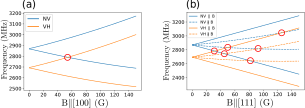
\includegraphics[width=0.9\textwidth]{chapter 2/Figures/121_vs_22_VH}
\caption{Simulation of the transition frequencies of NV$^-$ centers and VH$^-$ centers for a magnetic field a) along the [100] axis and b) along the [111] axis}
\label{121 vs 22 VH}
\end{figure}

VH$^-$, a much less abundant electronic spin than P1 center, has an electronic spin 1, with a spin Hamiltoninan very similar to that of the NV center. In particular it has the same symmetries being also a $C_{3v}$ defect, with a slightly smaller ZFS at $D_{VH} \approx 2700\ \rm MHz$ compared to $D_{NV}=2870\ \rm MHz$. 

Fig. \ref{121 vs 22 VH} shows the transition frequencies for the NV$^-$ and VH$^-$ ground state spin. Contrary to the P1 case, there is a co-resonance when $\mathbf{B} \parallel [100]$ for $B\approx 55\ \rm G$. When $\mathbf{B} \parallel [111]$, there are 6 co-resonance conditions between 30 and 130 G. A scan along the [111] in this case means that the peak signal will be $\sim 6$ times weaker than in the [100] case, and spread over multiple lines which might overlap between themselves or with other existing PL features.

The War1 spin mentioned previously is also an electronic spin 1 with (pseudo)-$C_{3v}$ symmetry and $D_{War1} \approx 2470\ \rm MHz$. This result in a similar behavior than VH$^-$ when it comes to the CR condition with NV centers.

\subsection{CR condition between NV$^-$ and and $^{13}$C-NV$^-$}
\label{sec NV-13c-NV}

\begin{figure}[h]
\centering
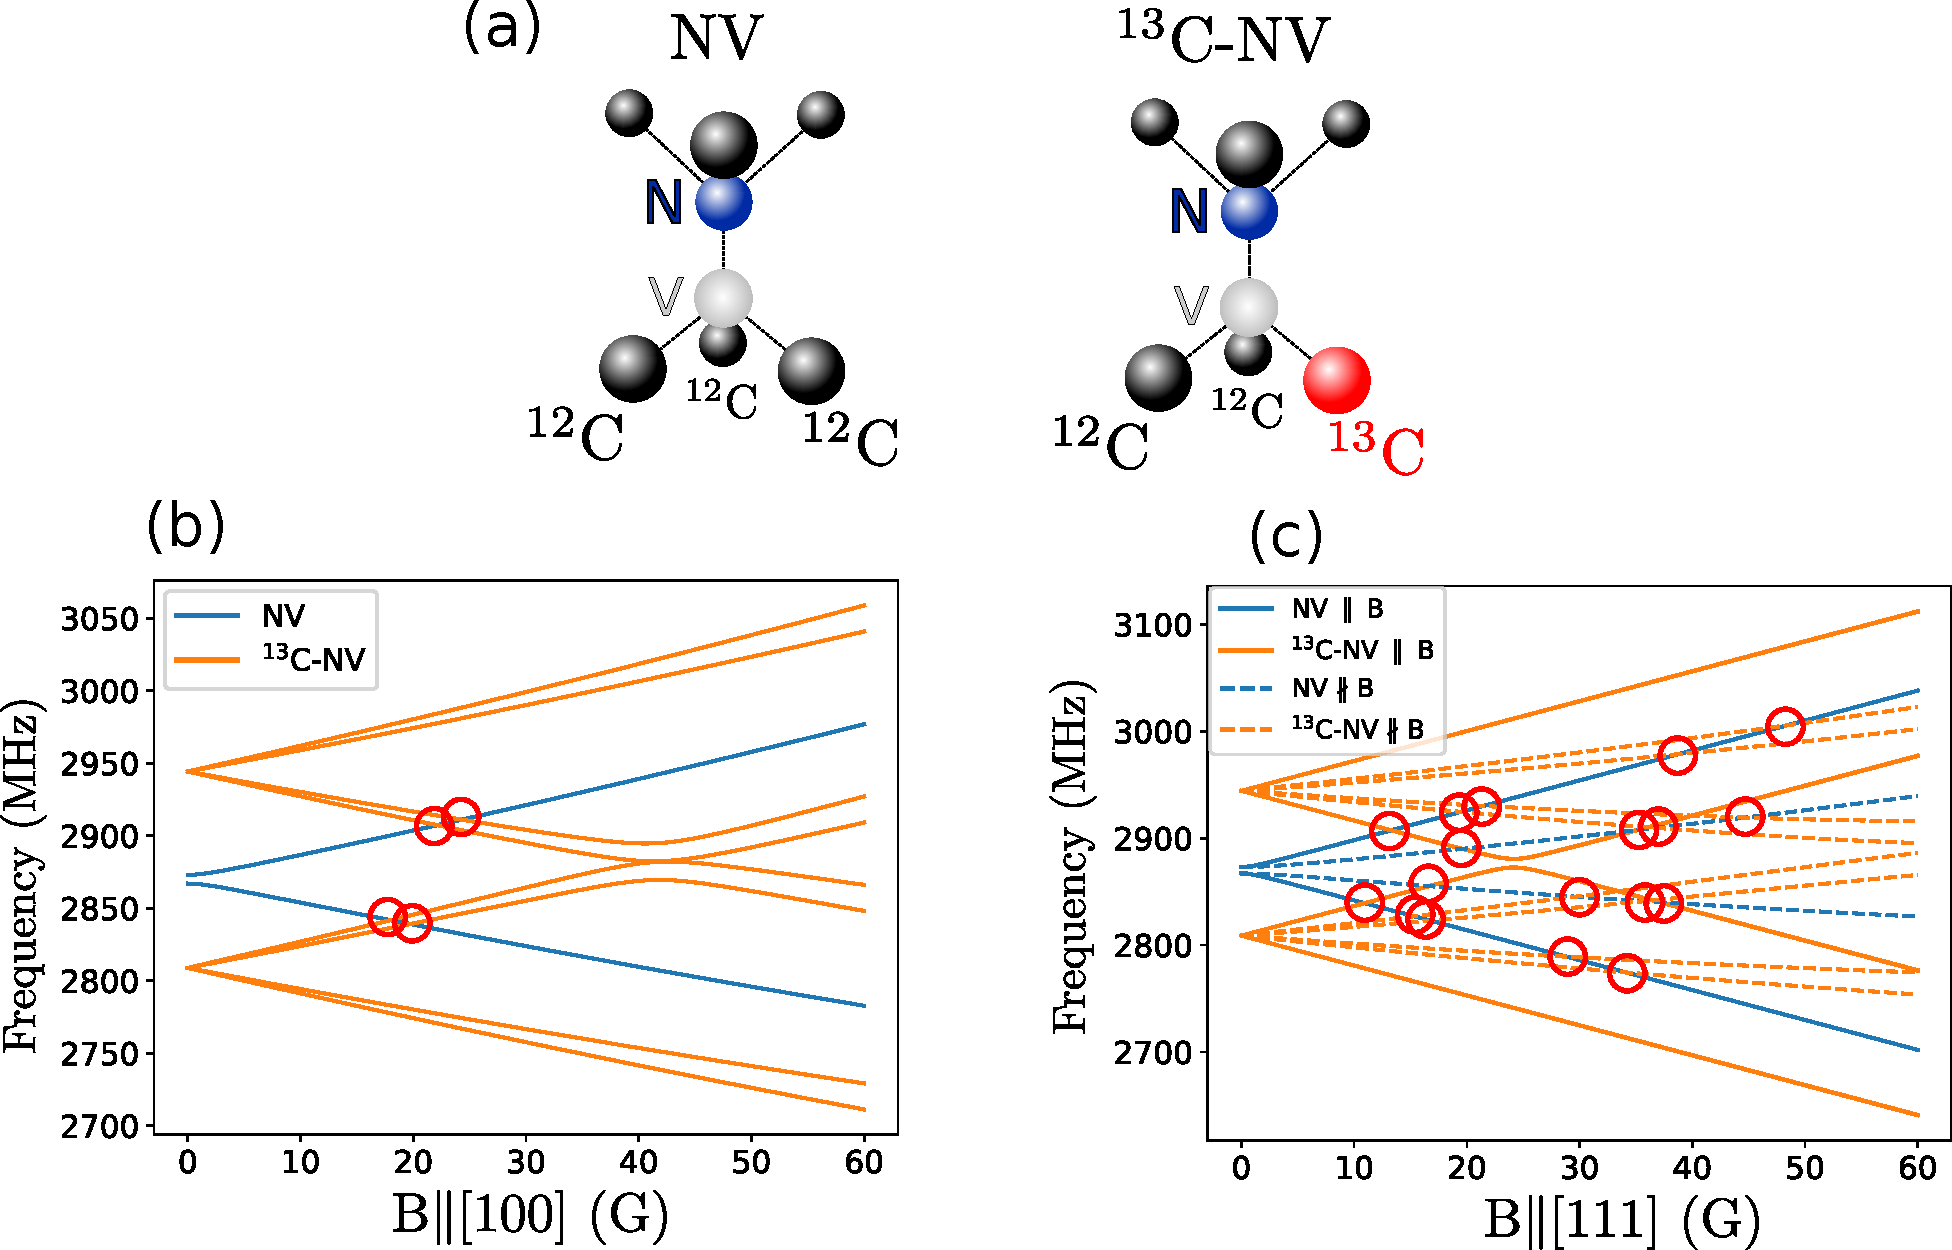
\includegraphics[width=1\textwidth]{chapter 2/Figures/121_vs_22_13CNV}
\caption{a) Representation of the $^{13}$C-NV complex (right) compared to a ``normal" NV center (left) b) and c) simulation of the transition frequencies of NV$^-$ centers and $^{13}$C-NV$^-$ complex for a magnetic field b) along the [100] axis and c) along the [111] axis}
\label{121 vs 22 13C-NV}
\end{figure}

The $^{13}$C-NV$^-$ complex is formed by an NV center where one of the three carbon atoms neighboring the vacancy is a $^{13}$C isotope. Such a complex is illustrated in Fig. \ref{121 vs 22 13C-NV}-a).

The $^{13}$C-NV$^-$ complex still behaves as a ``normal" NV center, except that its transition lines are shifted by the hypere-fin coupling. In particular its electronic spin is still polarized in the $\ket{0}$ state and the $\ket{0}$ state is still brighter than the $\ket{\pm 1}$ states\footnote{This is confirmed by the presence of sideband in ODMR spectra around the main NV lines \citep{simanovskaia2013sidebands}.}. 

Since both NV$^-$ and $^{13}$C-NV$^-$ are \textit{a priori} equally polarized, then following the argument in \ref{Sec_CR} there should be no CR between the two spin families. The reason why those transitions are still visible is the presence of dark NV-centers (``fluctuators") which will be further explained in chapter 3.

The transitions of the $^{13}$C-NV$^-$ complex are given by diagonalizing the full spin Hamiltonian:
\begin{equation*}
\mathcal{H}=\mathcal{H}_{NV}+\mathcal{H}_{^{13}C}+\mathcal{H}_{HF},
\end{equation*}
where $\mathcal{H}_{NV}$ is the NV$^-$ spin Hamiltonian,
$\mathcal{H}_{^{13}C}$ is the $^{13}$C nuclear spin Hamiltonian for a $1/2$ spin : $\mathcal{H}_{^{13}C}=\gamma_{n} B I_z$ where $\gamma_{n}=$10.7 MHz/T is the $^{13}$C gyromagnetic ratio, and $\mathcal{H}_{HF}$ is the hyper-fine interaction Hamiltonian: $$\mathcal{H}_{HF}= \hat{\mathbf{S}}_{NV} \cdot \mathcal{A} \cdot \hat{\mathbf{I}}_C.$$

When the $^{13}$C is the direct neighbor of the vacancy as represented in Fig. \ref{121 vs 22 13C-NV}-a) - this is also referred as a first-shell $^{13}$C - the hyper-fine tensor $\mathcal{A}$ can be written \citep{simanovskaia2013sidebands}:
$$ \mathcal{A} = \begin{pmatrix}
\mathcal{A}_{xx} & 0 & \mathcal{A}_{xz} \\ 0 & \mathcal{A}_{yy} & 0 \\ \mathcal{A}_{zx} & 0 & \mathcal{A}_{zz}
\end{pmatrix},$$
where $\mathcal{A}_{xx}=190$ MHz, $\mathcal{A}_{yy}=120$ MHz, $\mathcal{A}_{zz}=129$ MHz, and  $\mathcal{A}_{xz}=\mathcal{A}_{zx}=-25.0$ MHz. 

Fig. \ref{121 vs 22 13C-NV}-b) and c) show the simulated transition frequencies for a $^{13}$C-NV$^-$ complex when B is scanned along the [100] or [111] axis, as well as the ``normal" NV transitions and the co-resonance between those two. When $\mathbf{B} \parallel [100]$, there are 4 co-resonances between 18 and 25 G. When $\mathbf{B} \parallel [100]$ there are 18 of them between 10 and 60 G. This abundance of transitions for low ($<100\ \rm G$) magnetic field makes the experimental analysis quickly intractable in the second case.

There is one last aspect to take into account regarding the field orientation choice which is the impact of the transverse magnetic field on the cross-relaxation contrast.

\subsection{CR contrast and transverse magnetic field}
\label{CR contrast}

\begin{figure}[h]
\centering
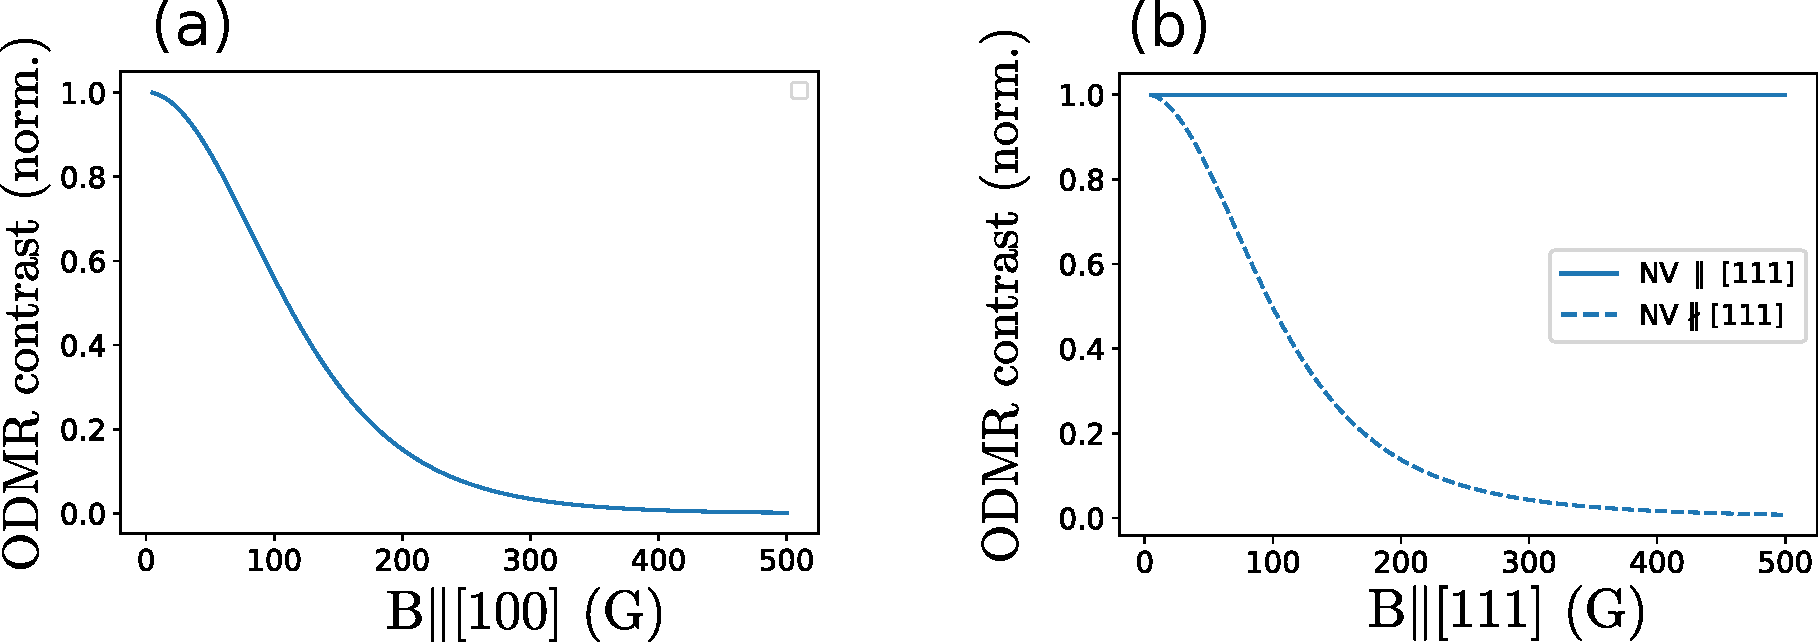
\includegraphics[width=0.9\textwidth]{chapter 2/Figures/contrast_OMDR_111_Vs_100}
\caption{Simulated ODMR contrast on all four classes of NV centers with a magnetic field a) along the [100] axis and b) along the [111] axis}
\label{121 vs 22 contrast}
\end{figure}

Similarly to ODMR, there are two required conditions to observe NV cross-relaxation on the PL signal: 
\begin{itemize}
\item There must be a difference in population between the two NV spin states involved in the CR (e.g. $\ket{0}$ and $\ket{-1}$), otherwise there would be no population transfer with the unpolarized dark spin.
\item The two NV spin states must have a difference brightness in order to be optically detectable.
\end{itemize}

These two conditions are fulfilled when there is no magnetic field or purely longitudinal magnetic field, but not anymore in the presence of transverse magnetic field which mixes the NV spin Hamiltonian eigenstates \citep{tetienne2012magnetic}.

Fig. \ref{121 vs 22 contrast} shows the simulated relative contrast of a CR process \footnote{Due to the similarity between ODMR and CR, we assume here that the ODMR contrast is equal to the CR contrast} computed from the rates found in \citep{tetienne2012magnetic}, for a magnetic field aligned along either [100] or [111]. When the NV center is aligned with the magnetic field, the contrast remains equal to 1 regardless of the magnetic field because there is no transverse field. When the NV is not aligned however, the CR contrast quickly drops down for B$>100\ \rm G$.

The [100] direction is therefore not well suited to observe CR at magnetic fields higher than a few hundreds gauss. Fortunately, the co-resonance between NV centers and VH$^-$, War1 or $^{13}$C-NV$^-$ all happen for $|\mathbf{B}| < 150 \ \rm G$, and can thus be detected with a [100] oriented magnetic field. 

\section{Dark spin spectroscopy with NV centers}
This section shows experimental observation of NV-dark spins CR. Previously to our work, several studies \citep{van1989cross, holliday1989optical, epstein2005anisotropic, armstrong2010nv,   hall2016detection, wickenbrock2016microwave,  wood2016wide,  alfasi2019detection, lazda2021cross} had been performed on the detection of dark spins through CR with NV centers, and to our knowledge, all this studies where done on the detection of P1 centers. 

We show an example of one this study to illustrate the principle of dark spin spectroscopy before showing our results on the detection of VH$^-$ and War1 in a CVD diamond.

\subsection{Detection of P1 centers}

\begin{figure}[h]
\centering
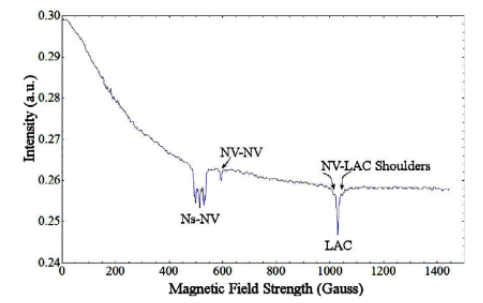
\includegraphics[width=0.7\textwidth]{chapter 2/Figures/NV_P1_libreAcces}
\caption{Change in the PL of an ensemble of NV centers as a magnetic field is scanned along the [111] crystalline axis. Taken from \citep{armstrong2010nv}}
\label{CR P1 exp}
\end{figure}

An example of a NV-P1 CR study (\citep{armstrong2010nv}) is shown in Fig. \ref{CR P1 exp}. It shows the evolution of the NV PL with respect to a magnetic field scanned along the [111] crystalline axis. There are several information to gather from this graph: First, one observes a slowly decaying PL envelope, which stabilizes to a plateau for $B\sim 1000\ \rm G$. This change in PL is caused by the transverse magnetic field acting on the three NV classes that are not aligned with the magnetic field. For $B \gtrsim 1000\ \rm G$, these three classes are fully depolarized which explains the plateau observed.

Second, there are three salient features denoted Ns-NV, NV-NV and NV-LAC. All these features come from cross-relaxations or level anti-crossing (LAC) from the NV class aligned with the magnetic field.

The first feature (Ns-NV) for $B\approx 512 \ \rm G$ is the signature of the CR between NV and P1 centers. Its relatively complicated shape comes from the hyper-fine coupling between the P1 electronic spin and the $^{14}$N nucleus \citep{lazda2021cross}. Excited state level anti-crossing (ESLAC) also occurs in this region, but its optical signature, if it exists, is expected to be much weaker than the NV-P1 CR \citep{zheng2017level}.

The second feature (NV-NV) for $B\approx 590 \ \rm G$ comes from the cross relaxation between NV centers aligned with the magnetic field and NV centers misaligned with the field (the co-resonance can be observed in Fig. \ref{121 vs 22 NV}-b)). This phenomenon will be further discussed in the next chapter.

Finally the third feature (LAC) for $B\approx 1024 \ \rm G$ correspond to the level anti-crossing between the $\ket{0}$ and $\ket{-1}$ states of the NV center aligned with B. When the two levels get close enough in energy, the Hamiltonian off-diagonal terms (coming from strain local electric field or residual transverse magnetic field) will mix the $\ket{0}$ and $\ket{-1}$ states and prevent an efficient polarization by the green laser. This result in a sharp drop in the PL that can be exploited to perform microwave-less magnetometry with NV centers \citep{wickenbrock2016microwave, zheng2017level, zheng2020microwave}.

\subsection{Detection of VH$^-$, War1 and $^{13}$C-NV$^-$}

\begin{figure}[h]
\centering
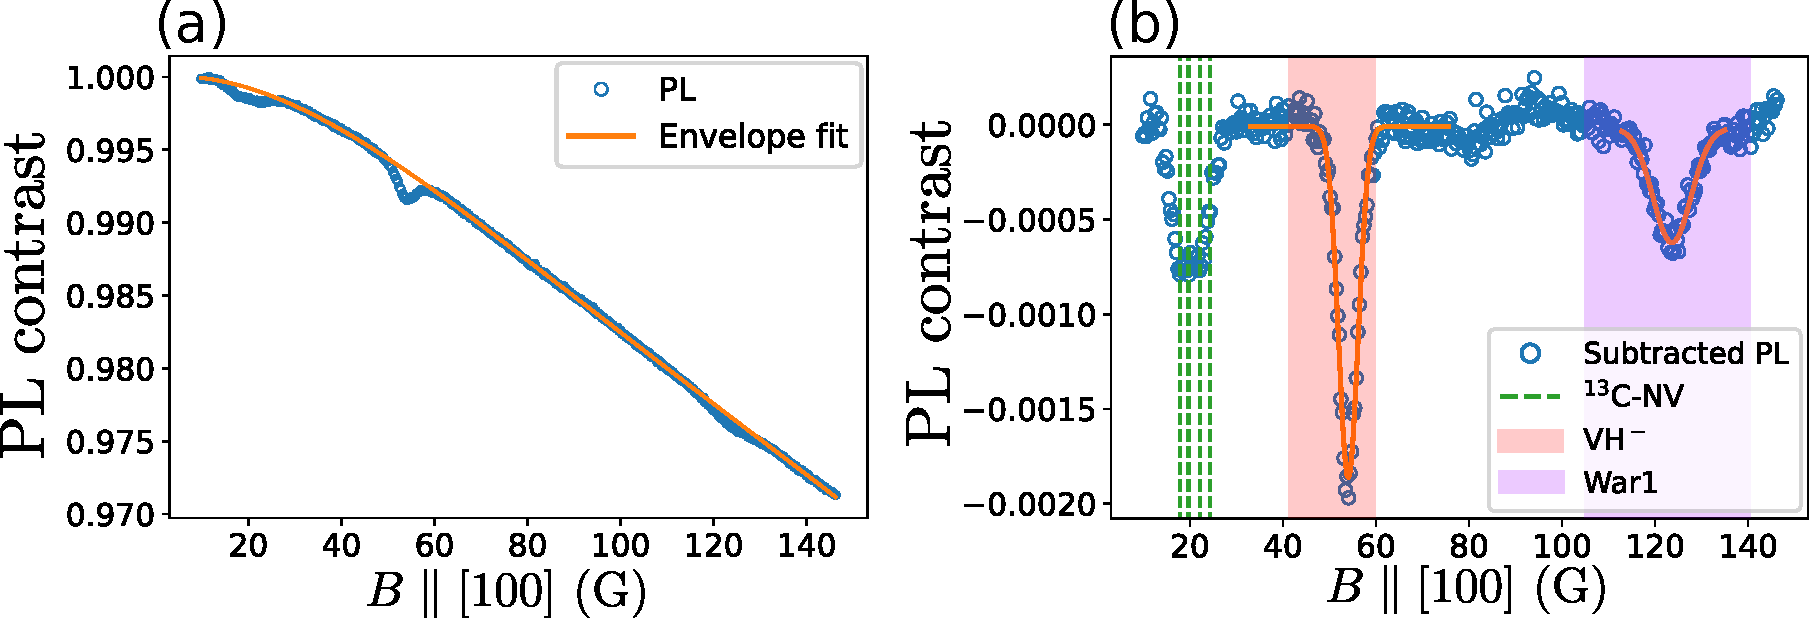
\includegraphics[width=\textwidth]{chapter 2/Figures/fig_VH_et_co}
\caption{a) Change in PL (normalized) of the ensemble of NV centers in sample CVD-pink as a magnetic field is scanned along the [100] axis. The orange line is a fit to the slowly decreasing envelope b) Subtraction of the PL signal by the envelope fit as a function of the magnetic field. The green lines and red and purple regions correspond to the predicted CR regions, as detailed in main text}
\label{CR VH exp}
\end{figure}

Our work \citep{pellet2021optical} focuses on the optical detection of VH$^-$, War1 and $^{13}$C-NV$^-$ through NV CR. This study was the first to detect VH$^-$ and War1 defects optically and the first CR experiment on a CVD diamond. It was also the first,to our knowledge, to use a [100] aligned magnetic field.

The diamond used for this study is the sample CVD-pink (see sample details in appendix \ref{Appendix samples}). The experimental setup used to obtain this data is the standard confocal microscopy setup shown in Sec \ref{Sec setup cahp 1}. The magnetic field here is generated with an electromagnet (EM), aligned along the [100] diamond axis with a precision $<1^\circ$. 

Fig. \ref{CR VH exp}-a) shows the change in PL with respect to a magnetic field scanned along the diamond [100] axis. Similarly to fig. \ref{CR P1 exp}, there is a slowly decaying envelope of the PL due to the transverse magnetic field \footnote{The plateau is not visible in this case as the scan stops at 150 G}. There also are three deviations from the smooth decreasing curve at $\sim$ 20 G, 55 G and 120 G.

In order to better discern the three features, we fitted the envelope with a polynomial fit of order 4. We previously tried to simulate the PL dependency on the transverse field  by using the model in \citep{tetienne2012magnetic}, but the result did not correctly fit our data.

Fig. \ref{CR VH exp}-b) shows the subtraction of the PL data by the envelope fit. We can clearly see three dips in PL around the values 20 G, 56 G and 122 G. We then computed the expected value of the magnetic field for the expected CR line thanks to the simulations shown in sec. \ref{sec simu}. For the VH$^-$ and War1 lines, we took the ZFS $D$ values from \citep{cruddace2007magnetic} and included the error bars. For the $^{13}$C-NV$^-$ lines, the error bars given in \citep{simanovskaia2013sidebands} are much smaller and we only plotted the expected value. We can see that the dips in PL match relatively well the predicted CR lines of $^{13}$C-NV$^-$, VH$^-$ and War1 respectively.

The data shown here was acquired over 24 h. It should be noted however that a single-photon counting APD was used for this acquisition, which reduces significantly the sensitivity because of the high shot noise \footnote{The sample produces $\sim$ 100 nW of PL, which means that only $\sim 10^{-5}$ of the total PL is actually measured by an SPC-APD with a max counting rate of $10^7$ photons/s.}. Using a photodiode and modulation of the magnetic field, we estimate that we could get similar signal to noise ratio within a few minutes.

To calibrate the magnetic field, we added a microwave field at a  fixed frequency $\nu > 2870\ \rm MHz$, and measured the EM voltage at which the PL dropped due to the $\ket{+1}$ state of the NV centers becoming resonant with the microwave tone. We could then use the values in Fig. \ref{121 vs 22 NV} to find the corresponding magnetic field. We varied the frequency in the range  $[2870,3150]\ \rm MHz$ by step of 2 MHz to get a calibration of the magnetic field in the $[0,150]\ \rm G$ region. Considering the uncertainty in the field angle, the NV ZFS $D$ value and the width of the PL drop, we estimate the final precision of the calibration to be within $\pm 1\ \rm G$.

\section{Identification of the $^{13}$C-NV$^-$, VH$^-$ and War1 lines}

\subsection{The VH$^-$ and War1 lines}
\begin{table}[htbp]
\centering
\caption{\bf Zero-field splitting parameter $D$ for NV$^-$, VH$^-$ and War1}
\begin{tabular}{ccc}
\hline
$D_z$ estimation (MHz) & Cruddace's work\citep{cruddace2007magnetic} & Our work \\
\hline
NV$^-$ & 2872(7) & * \\
VH$^-$ & 2706(30) & 2694(5)  \\
WAR1 & 2466(60) & 2470(10) \\
\hline
\end{tabular}
  \label{table VH et War1}
\end{table}

The identification of the PL dips at 56 and 122 G in Fig. \ref{CR VH exp} as CR between NV and respectively VH$^-$ and War1 comes from two main observations: the closeness in the ZFS values, and the CVD nature of the sample.

Table \ref{table VH et War1} shows the value and precision of the $D$ factor when measured through EPR \citep{cruddace2007magnetic}, and when computed from the data in Fig. \ref{CR VH exp}. In order to get to the $D$ value of VH$^-$ and War1, we had to assume that the spin structure was that of a spin 1 similar to the NV center, with a g-factor close to 2. Both of this assumptions are confirmed by the EPR measurements. We do find that that both $D$ measurement concord within their respective error bars.

The second reason comes from the nature of the sample used. We tried similar PL scans along the [100] axis on many samples with dense ensemble of NV centers. We found that the dip at 55 G was present on all CVD samples ($\sim$ 5 samples) used, and none of the HPHT samples ($\sim$ 20 samples). The same is true of the 122 G line, except that it did appear on some HPHT samples, as will be discussed below. We know that the VH$^-$ defect is much more likely to appear in a CVD sample due to the large quantity of hydrogen used in the growth process, and while we do not know the chemical nature of the War1 defect, the only time it was observed through EPR was on a CVD diamond.

Finally, the apparent larger linewidth of the War1 line compared to the VH$^-$ one is also corroborated by the EPR measurements.

For all of this reasons we attribute the 55 and 122 G dip to CR with VH$^-$ and War1 respectively.

\subsection{The $^{13}$C-NV$^-$ lines}

\begin{figure}[h]
\centering
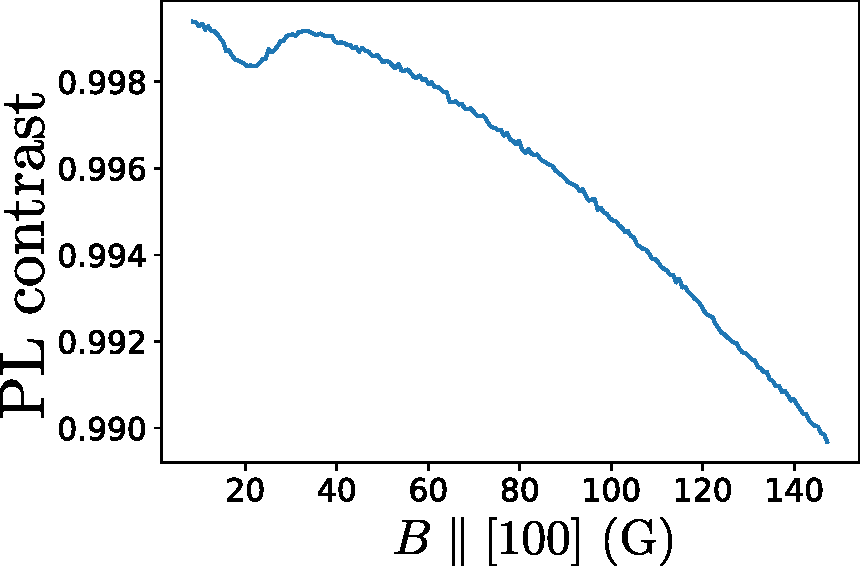
\includegraphics[width=.6\textwidth]{chapter 2/Figures/scan_100_Sumi4}
\caption{Change in PL as a function of a magnetic field scanned along the [100] axis for sample SUMI-4}
\label{scan sumi 4}
\end{figure}

The identification of the $\sim 20\ \rm G$ as CR between $^{13}$C-NV$^-$ and ``normal" NV centers also come from two observations. First, the lines are present on every single sample with dense ensemble ($\gtrapprox 1$ ppm), regardless of the fabrication process. Fig. \ref{scan sumi 4} for example shows a PL scan along the [100] axis for sample Sumi-4, an HPHT sample with [NV]$\approx 5\ \rm ppm$ and natural abundance of $^{13}$C \footnote{We could unfortunately not try a sample isotopically enriched in $^{12}$C since those samples are generally reserved to low-nitrogen concentration ($< 10\ \rm ppm$), which does not yield enough NV centers to perform CR spectroscopy. }. 

The second reason is the shape of the PL dip. The two other dips seem be formed of a single line and are reasonably well fitted with Gaussian curves. The 20 G dip however has a flat bottom which would indicate the presence of several overlapping lines, and Fig. \ref{121 vs 22 13C-NV} indeed predicts that there would be 4 CR lines between 18 and 25 G.

For this two reasons, we attribute the 20 G line to CR between $^{13}$C-NV$^-$ and ``normal" NV centers.

\bigskip

The CR spectra shown in this section can be used to detect the presence of particular impurities in the sample, but more quantitative information on these impurities can also be extracted from these spectra, which is the object of the following section.

\section{Quantitative estimates of the NV-Dark spins CR}

This section exploit the CR spectrum shown in Fig. \ref{CR VH exp} in order to extract information on the dark spins Hamiltonian parameters, linewidth and concentration.

\subsection{Dark spin Hamiltonian parameters}

First, as discussed in the last section, we can estimate the dark spin ZFS $D$ value with greater precision than EPR. While it would be in theory possible to measure other properties of the dark spins Hamiltonian - such as the $g$-factor - by changing the angle of the magnetic field, this would here quickly become intractable due to the increase in co-resonance conditions and the relative closeness of each of these transitions. DEER might prove more useful in this regard as only one class of NV centers at a time is probed.

\subsection{Dark spin linewidth}

The second quantitative estimate we can make is of the dark spin inhomogeneous broadening $T_2^*$: if we assume the change in PL to be proportional to the change in the NV lifetime $T_1$, which is true for small enough changes, then the linewidth of the PL dips in Fig. \ref{CR VH exp} is the convolution of the NV and dark spin spectrum. By deconvoluting the data with the NV spectrum, known for example from ODMR, we can then recover the dark spin spectral response as was done in \citep{hall2016detection}. 

This procedure will be discussed in more details in the next chapter. We find here that the linewidth of VH$^-$ and War1 are respectively (half width at half maximum) $5.7\pm 0.6$ and $15.7\pm 1.6$ MHz \footnote{We follow here the pseudo-Voigt deconvolution method described in the following chapter. The linewidth $W=2.7$ MHz (half witdth at half maximum) of the NV centers was measured from ODMR (see Fig. \ref{ODMR 1 classe}). It includes all three hyper-fine transistions}.

\subsection{Dark spin concentration}

Finally, the third estimate we can make is that of the dark spins concentration. We can indeed calibrate the measurement by using the $^{13}$C-NV$^-$ line, of which we know the concentration in natural abundance diamond: [$^{13}$C-NV$^-$] $\approx$ 3.3 \% [NV]. We can then, knowing the NV concentration, try to estimate the concentration of the dark spins. There are however several caveats:

\begin{itemize}
\item Since the change in $T_1$ is proportional to the $T_2^*$ of the probed spins (eq. \ref{delta gamma 1}), we should compensate that by integrating over the entire feature, instead of simply looking at the maximum of the line.
\item We have to take into account the loss of contrast of the NV centers as the transverse magnetic field grows, as explained in sec. \ref{CR contrast}.
\item The $^{13}$C-NV$^-$ are not ``dark spins", and its CR feature cannot be \textit{a priori} compared to the one from VH$^-$ and War1. We will see however in the next chapter that we can consider a fraction of the NV centers as dark spins, and that this fraction can be estimated. \citep{choi2017depolarization} found a ratio of $\sim 1/4$ dark NV centers for $\sim 3/4$ bright ones.
\end{itemize}

From these considerations, we can give an estimate of the concentrations of VH$^-$ and War1 based on the data on Fig. \ref{121 vs 22 VH}-b): 

For the VH$^-$ line we find that the area of the line is $\approx 1.4$ times bigger than that of the $^{13}$C-NV$^-$ one, from \ref{121 vs 22 contrast} we find that the expected CR contrast is $\approx 1.2$ times smaller at 55 G than at 20 G, and finally we chose a dark to bright NV ratio of 0.25 as found in \citep{choi2017depolarization}.

With an estimated NV concentration [NV] $\approx\ \rm 4.6 ppm$, giving us a concentration $[^{13}\rm{C-NV}^-]\approx \ \rm 130 ppb$, we then find $[\rm VH^-] \approx 58\ \rm ppb$. Similarly, we find $[\rm VH^-] \approx 68\ \rm ppb$. Given the large uncertainty on some parameters, in particular the dark to bright spin ratio, these estimates are probably only precise within an order of magnitude.

If we consider that the sampled volume in this experiment is $< 100 \mu \rm{m}^3$, the total number of dark spins detected here is then $< 10^6$. Even with very conservative estimates, the technique employed here is still more sensitive than EPR by several orders of magnitude.

\section{Temperature dependence of VH$^-$ and War1}


\subsection{Mofifications on CVD samples}
\begin{figure}[h]
\centering
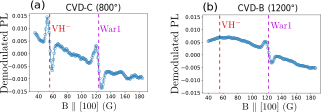
\includegraphics[width=\textwidth]{chapter 2/Figures/VH_CVD_chauffage}
\caption{Demodulated PL on samples CVD-C and CVD-B as a function of a magnetic field along the [100] axis. An additional oscillating magnetic field along the same direction was used to perform the lock-in detection. The VH$^-$ and War1 lines are taken from \ref{CR VH exp}}
\label{chauffage CVD}
\end{figure}

Given that the NV CR spectroscopy was both sensitive and relatively easy to setup, we decided in collaboration with the teams of Alexandre Tallaire at IRCP and Jocelyn Achard at LSPM to study the effect of annealing at high temperature on VH$^-$ and War1 \citep{ngambou2022improving}.

Fig. \ref{chauffage CVD} shows the results of this experiment. This time, a modulation of the magnetic field was used and the PL coming from the photodiode was demodulated through a lock-in amplifier, which explains the derivative shape of the lines. The fact that the background is not perfectly flat still comes from the transverse magnetic field. The same lock-in parameter were used on both plots so that the amplitudes should in theory be comparable.

Fig \ref{chauffage CVD}-a) shows the demodulated PL versus mganetic field amplitude along [100] on sample CVD-C, while \ref{chauffage CVD}-b) shows the same experiment on sample CVD-B. The fabrication and subsequent operations done on this two samples are detailed thoroughly in \citep{ngambou2022improving}, but the main difference between these two sample is that CVD-C was only annealed once after irradiation, for 2 hours at 800$^\circ$C, while CVD-B was annealed for 2 hours at 800$^\circ$C and then for 1 hour at 1000$^\circ$C and 1 hour at 1200$^\circ$C.

We can see that the VH$^-$ line in particular completely disappears on sample CVD-B, which we attribute to the additional annealing. This measurement also corroborate modifications in the infrared absorption spectrum, and an increase of the NV coherence time, associated with the annealing at higher temperature \citep{ngambou2022improving}.

The War1 line on the other hand is still present after the high temperature annealings, albeit slightly smaller. This information can give us some insights on the chemistry of the War1 defect. %Et en vrai je crois que c'était deja vu dans la thèse de Cruddace

\subsection{Modification on HPHT samples}

\begin{figure}[h]
\centering
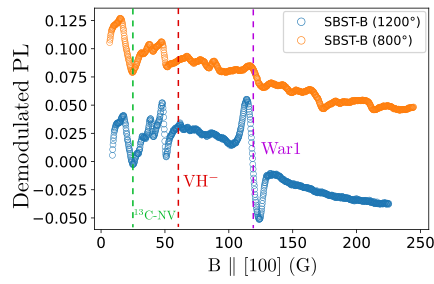
\includegraphics[width=.7\textwidth]{chapter 2/Figures/VH_HPHT_chauffage}
\caption{Demodulated PL on samples SBST-C and SBST-B as a function of a magnetic field along the [100] axis. The plot of SBST-C is offset for clarity}
\label{chauffage HPHT}
\end{figure}

An unexpected side-study was done on HPHT samples. Indeed, the CVD samples used previously are grown by homoepithaxy on top of a diamond substrate. In this case, the substrate was a type 1B HPHT diamond, which was irradiated and annealed along the CVD layer. We will name SBST-C and SBST-B the respective HPHT substrate of CVD-C and CVD-B.

Fig. \ref{chauffage HPHT} shows demodulated PL scans with B $\parallel$ [100] on both samples. They both show a line at $B \approx 20\ \rm G$ corresponding to the $^{13}$C-NV$^-$ line, and none of them show a line at $B = 56\ \rm G$ corresponding to the VH$^-$ line. There is however a stark difference for the War1 line: SBST-C seems to show a weak line, while SBST-B shows a very clear line, with an amplitude more than 5 times greater than SBST-C. 

We can also see that many weak lines on SBST-B seems to have disappeared in SBST-C, while an unidentified line at $B = 48\ \rm G$ seems to have grown similarly to the War1 line.

We first suspected that some of the War1 defects had been migrating from the CVD layer to the HPHT substrate with the high-temperature annealing, but not only is it very unlikely with the annealing time (1 hour) and substrate thickness (several mm), We also could not find a dependence on the War1 concentration with the depth in the substrate, whereas a diffusion would have given a higher concentration near the CVD layer. The War1 defects seem to have been created by the annealing.

These results suggest that, while some defects are removed by the high temperature annealing, such as the VH$^-$ and several unidentified defects in the HPHT substrate, some seem to be created by the annealing process, such as the War1 or the one associated with the line at $B = 48\ \rm G$ in the HPHT substrate.

\section{Conclusion and perspectives}

To conclude this chapter, we have seen how NV centers can be used to detect dark spins via cross-relaxations. This detection can be significantly more sensitive than the usual EPR spectroscopy, and considerably cheaper to set up. This technique however is only applicable to a few defects in NV-rich diamond, meaning that its main application would probably be to characterize the environment of samples with high NV density.

We have also seen the importance of the magnetic field direction, and the underused aspect of the [100] magnetic field scan which provides a significantly less noisy signal than the [111] scans for weak magnetic field.

Finally we have seen an application of the CR to detect and characterize optically two dark spins in CVD diamond, and to find out the response of these defects to high temperature annealing.

There still remains a lot of open questions and there are several experiments that could be build upon these results. Some of these questions are listed below.

\subsection{Unidentified CR lines}

There are still a large number of lines in CR spectra that have not been identified. While not every line necessarily correspond to a new defect - for example \citep{wunderlich2021magnetic} recently found lines corresponding to co-resonance between the $\ket{0} \to \ket{-1}$ transition of an NV center and the $\ket{-1} \to \ket{+1}$ of another NV center - the more likely hypothesis for each of these unidentified lines is still the presence of a new defect.

Such unidentified lines can be seen in Fig. \ref{chauffage CVD} and \ref{chauffage HPHT}. In particular we can see a line at 160 G in Fig. \ref{chauffage CVD}-a) and a line at 48 G in Fig. \ref{chauffage HPHT} that detach clearly from the background. 

Further studies would be needed to find how common these lines are, and what could be there sources.

\subsection{Measuring the spin dynamics of VH$^-$}

We found that NV-VH$^-$ CR in CVD could produce a change in PL of $\sim 0.2 \%$. This value is within one order of magnitude from ODMR contrast with NV ensembles (typically $<5 \%$), which means that it would be reasonable to probe the dynamics ($T_1$, $T_2$) of the VH$^-$ spin. The main issue comes from the fact that in order to measure the VH$^-$ spin states, it needs to be resonant with the NV center. Therefore, resonant microwave pulses with VH$^-$ will also be resonant with the NV centers, which will create an unwanted optical signal.

There are two solution to circumvent this problem: the first is to use a fast switching magnetic field in order to bring the VH$^-$ and NV centers in resonance when initializing or reading out the VH$^-$ state, and out of resonance to coherently manipulate the VH$^-$. This means that the magnetic field needs to be switched faster than the probed spin dynamics, which may be doable for the population dynamics $T_1$ but is likely too slow to probe the $T_2$ time.

The other solution consists in using the spin-1 nature of VH$^-$: when a NV$^-$-VH$^-$ CR occurs, only one of the transitions of VH$^-$ and NV$^-$ is brought to resonance. The other one ($\ket{0} \to \ket{-1}$ for the VH$^-$ and $\ket{0} \to \ket{+1}$ for the NV) is out of resonance. The idea would therefore be to keep the NV $\ket{0} \to \ket{-1}$ transition and VH $\ket{0} \to \ket{+1}$ transition resonant, and to coherently manipulate the VH $\ket{0} \to \ket{-1}$ transition. Further studies are needed to assess the effectiveness of this scheme.

\subsection{Isolating a single VH$^-$}

We estimated the concentration of VH$^-$ in CVD-pink to be $\sim 60\ \rm ppb$. This concentration is about two orders of magnitude too high to contemplate isolating a single emitter with a diffraction-limited microscope. We know however that we can reduce the VH$^-$ concentration arbitrarily by applying high temperature annealing. We could therefore reduce the VH$^-$ concentration to be in the $0.1 \sim 1\ \rm ppb$ range and optically isolate a single VH$^-$ center by scanning a confocal microscope with a fixed $B_{[100]}=56\ \rm G$ while monitoring the NV PL or $T_1$. It is however still unclear whether the present detection scheme is sensitive enough to detect single VH$^-$.


\chapter{NV-NV cross-relaxations : the fluctuator model}
This chapter will cover cross-relaxations between NV centers in the non-zero magnetic field regime, both from an experimental and theoretical point of view. The case of zero magnetic field will be treated in the next chapter.

The presence of strong NV-NV dipolar interaction in dense ensemble ([NV] $\gtrsim 1\ \rm ppm$) proved to be both an obstacle for ensemble magnetometry \citep{zhou2020quantum} and an opportunity to explore and use the many-body interaction resulting from it \citep{zhou2020quantum, choi2017observation, kucsko2018critical, zu2021emergent}.

We will see in this chapter how a model of fast and slow relaxing centers, the fluctuator model \citep{choi2017depolarization}, explains most observations related to the cross-relaxation, including the stretched exponential lifetime profile and the spectral broadening of the interaction.

\section{Experimental observation of NV-NV CR}
Let us start with the experimental proof of the presence of NV-NV CR in the samples with dense NV ensembles.

We make the distinction between what we will label ``equivalent" and ``non-equivalent" NV centers. Two equivalent centers are NV centers with the same spin Hamiltonian (cf eq. (\ref{eq. spin elec})), which implies that they both see the same transverse and longitudinal magnetic field. In contrast, non-equivalent centers are center with different single-spin Hamiltonian, which may result in different eigenstates and spin polarization for the two spins.

While the NV physics can explain cross-relaxations between non-equivalent NV centers, it cannot explain cross-relaxation between equivalent NV centers. Nevertheless, as we will see in this section, CR between both equivalent and non-equivalent NV centers is observed for samples with high NV density. 
\subsection{NV-NV CR between non-equivalent NV centers}
\label{non_equi_valent_CR}
\begin{figure}[h]
\centering
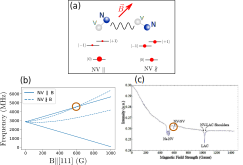
\includegraphics[width=\textwidth]{chapter 3/Figures/NV-NV_non_equivalent}
\caption{a) Illustration of the four possible direction of the the NV axis (four classes of NV centers) with a magnetic field along class 1 b) Representation of the polarization of two non equivalent spins, one aligned with the magnetic field (well polarized) and one misaligned with the magnetic field (unpolarized). c) Simulated frequencies for the $\ket{0} \to \ket{-1}$ and $\ket{0} \to \ket{+1}$ transitions when $\mathbf{B}\parallel [111]$ for the class aligned with B, and the 3 equivalent classes not aligned with B. d) Taken from \citep{armstrong2010nv}, PL change of an ensemble of NV centers as a magnetic field is scanned along the [111] axis.}
\label{non-equivalent NV-NV}
\end{figure}

In the absence of magnetic gradient, two NV centers can only be non-equivalent if the projection of the magnetic field upon their respective NV axis is different. Fig. \ref{non-equivalent NV-NV}-a) illustrates such a case: we label here the four possible NV axis orientation (or NV classes) 1 to 4 and we assume that the magnetic field is aligned with class 1. In this conditions, an NV center belong to class 1 will always be non-equivalent with NV centers from classes 2-4, as the projection of the magnetic field on their respective axis will never be the same. On the other hand, NV centers from the classes 2-4 are all equivalents, even though they do not necessary belong to the same class.

Fig. \ref{non-equivalent NV-NV}-b) shows the difference between the NV centers belonging to class 1 (labeled NV$_\parallel$) and those belonging to classes 2-4 (labeled NV$_\nparallel$). As explained in sec. \ref{sec champs transverse}, the transverse magnetic field leads to a mixing of the eigenstates \footnote{The states of the misaligned NV on Fig. \ref{non-equivalent NV-NV}-b) are labeled $\ket{0},\ket{\pm 1}$ which is an abusive (but common) notation since the mixing caused by the transverse field means that the eigenstates of $S_z$ are no longer the Hamiltonian eigenstates.} and to a loss of the optical polarization mechanism. As a result, the NV$_\nparallel$ spins are less polarized than the NV$_\parallel$ ones, which is a necessary condition to observe cross-relaxation.

Another necessary condition to observe cross-relaxation is the condition of co-resonance. In most situations, non-equivalent NV centers are not co-resonant, as the differences in the spin Hamiltonian generally leads to different eigenvalues. This is in contrast with equivalent NV centers which are by definition always resonant. Fig. \ref{non-equivalent NV-NV}-c) shows the transition frequencies of spin from class 1 and a spin from class 2-4 as a function of the magnetic field amplitude. Unintuitively, there is a co-resonance between the two $\ket{0} \to \ket{+1}$ transitions for $\abs{\mathbf{B}}=592\ \rm G$. For this particular value of the magnetic field, cross-relaxation between the NV centers from class 1 and those from classes 2-4 is possible.

Finally, Fig. \ref{non-equivalent NV-NV}-d), which was presented in the last chapter, shows the experimental value of the total NV PL as a function of the magnetic field amplitude, in a scenario similar to the one we just described. We can indeed observe the signature of NV-NV CR in the presence of a PL dip at $\abs{\mathbf{B}}=592\ \rm G$.

As previously mentioned, cross-relaxation between non-equivalent NV centers is easily explained by the physics of single NV centers, and has been known for more than thirty years \citep{holliday1989optical, van1989cross}.

\subsection{NV-NV CR between equivalent NV centers}

\begin{figure}[h]
\centering
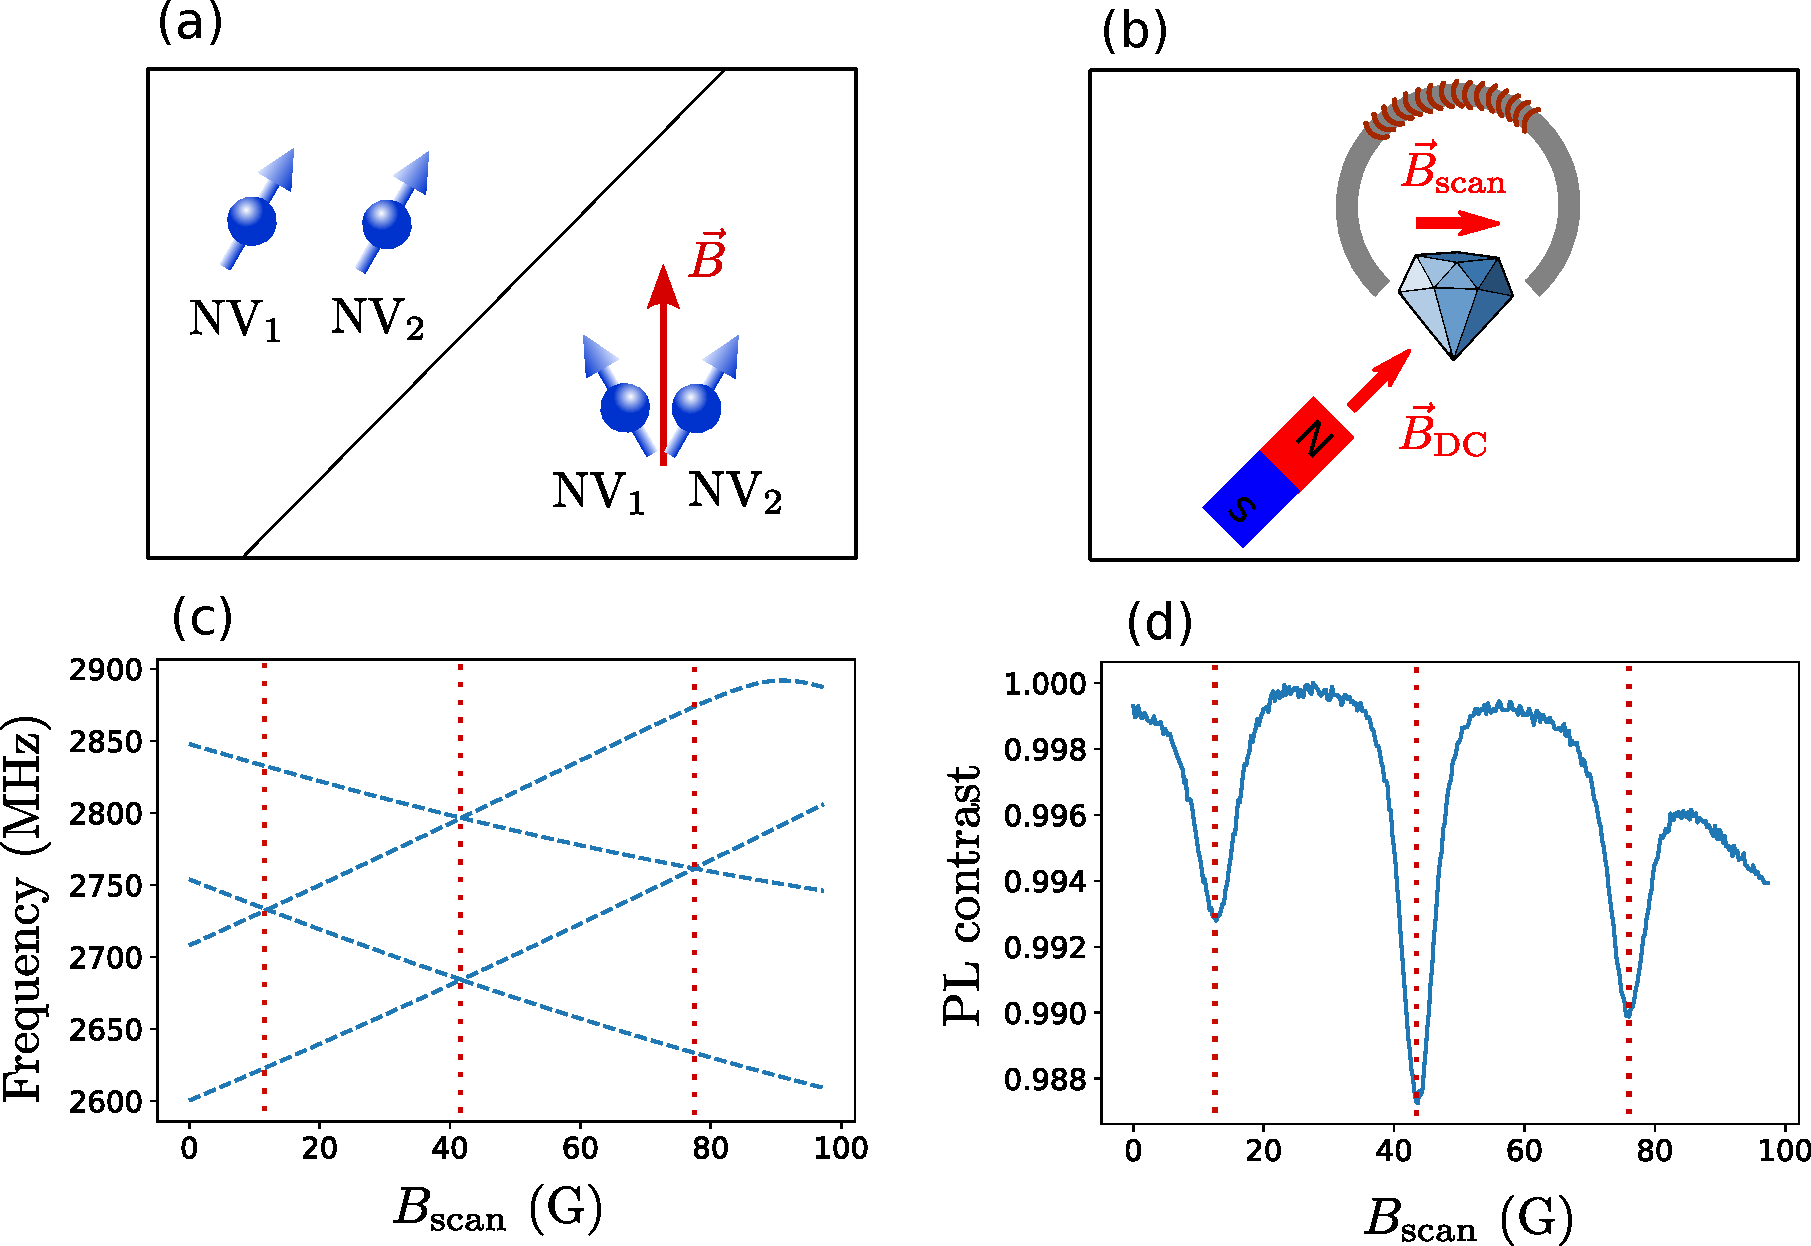
\includegraphics[width=\textwidth]{chapter 3/Figures/NV-NV_equivalent}
\caption{CR between equivalent NV centers for sample ADM-15-1. (a) Representation of equivalent NV centers: either two NVs from the same class, or two classes with the same projected magnetic field. (b) Magnetic setup used for the experiment: a permanent magnet is used to apply a bias magnetic field, and an electromagnet is used to add a variable magnetic field. (c) Simulation showing the $\ket{0}\to\ket{-1}$ transition frequencies for the 4 classes of NV centers as a function of the scanned magnetic field. The transitions were computed based on ODMR spectra recorded for different magnetic field values. (d) Change in the PL of the NV centers ensemble as a function of the scanned magnetic field.}
\label{equivalent NV-NV}
\end{figure}

More recently, experiments on dense NV ensemble ($[\rm NV ] >1\ \rm ppm$) or at low temperature have shown that there were cross-relaxations even between equivalent NV centers \citep{jarmola2012temperature, mrozek2015longitudinal, jarmola2015longitudinal, choi2017depolarization}.

Fig. \ref{equivalent NV-NV}-a) illustrates the two possible scenarios for equivalent NV centers: either two NVs from the same class, or two NVs from different classes with the same projection of the magnetic field upon their respective axis (i.e. $\mathbf{B}$ belongs to the plane of mirror symmetry of the two spins). 

In the second case, by moving the magnetic field in and out of the symmetry plane, we can change the resonance condition between the two NV classes and measure the contribution of NV-NV cross-relaxation to the NV PL and spin lifetime. To do so, we need to add an initial bias magnetic field in addition to the scanned magnetic field, as represented in Fig. \ref{equivalent NV-NV}-b). %When doing so, the magnetic field felt by the diamond won't have a fixed orientation during the scan, and when the magnetic field crosses certain crystalline planes (detailed below), its projection on two or more classes of NV centers will be the same.

Fig. \ref{equivalent NV-NV}-c) shows the transition frequencies of the $\ket{0}\to\ket{-1}$ transition for the 4 classes of NV centers on sample ADM-15-1, an HPHT micro-diamond with $[\rm NV]\sim 3\ \rm ppm$. There are three magnetic field values $B_{\rm scan} \approx$ 12, 42 and 77 G for which there is an inter-class resonance. These values are reported in the figure with red dotted lines. Unlike the case presented in Fig. \ref{non-equivalent NV-NV}, all the inter-class resonances reported in Fig. \ref{equivalent NV-NV}-c) are between equivalent classes.

Finally, Fig. \ref{equivalent NV-NV}-d) shows the PL contrast as the electromagnet field is scanned. There are 3 very clear dips when $B_{\rm scan} \approx$ 12, 42 and 77 G which coincide with inter-class resonances. We will see later that this PL dip is associated with a decrease of the NV centers spin $T_1$ time from both classes.

This observation, and similar ones made by many groups \citep{jarmola2012temperature, mrozek2015longitudinal, choi2017depolarization, akhmedzhanov2017microwave, giri2018coupled}, seem to indicate that there are CR between equivalent NV centers. This is however incompatible with our previous assumptions that equivalent NV centers are equally polarized and bright. To understand this phenomenon, we will need to introduce new hypotheses.

\section{NV inhomogeneity and the fluctuator model}

\subsection{CR in an inhomogeneous NV bath}
\begin{figure}[h]
\centering
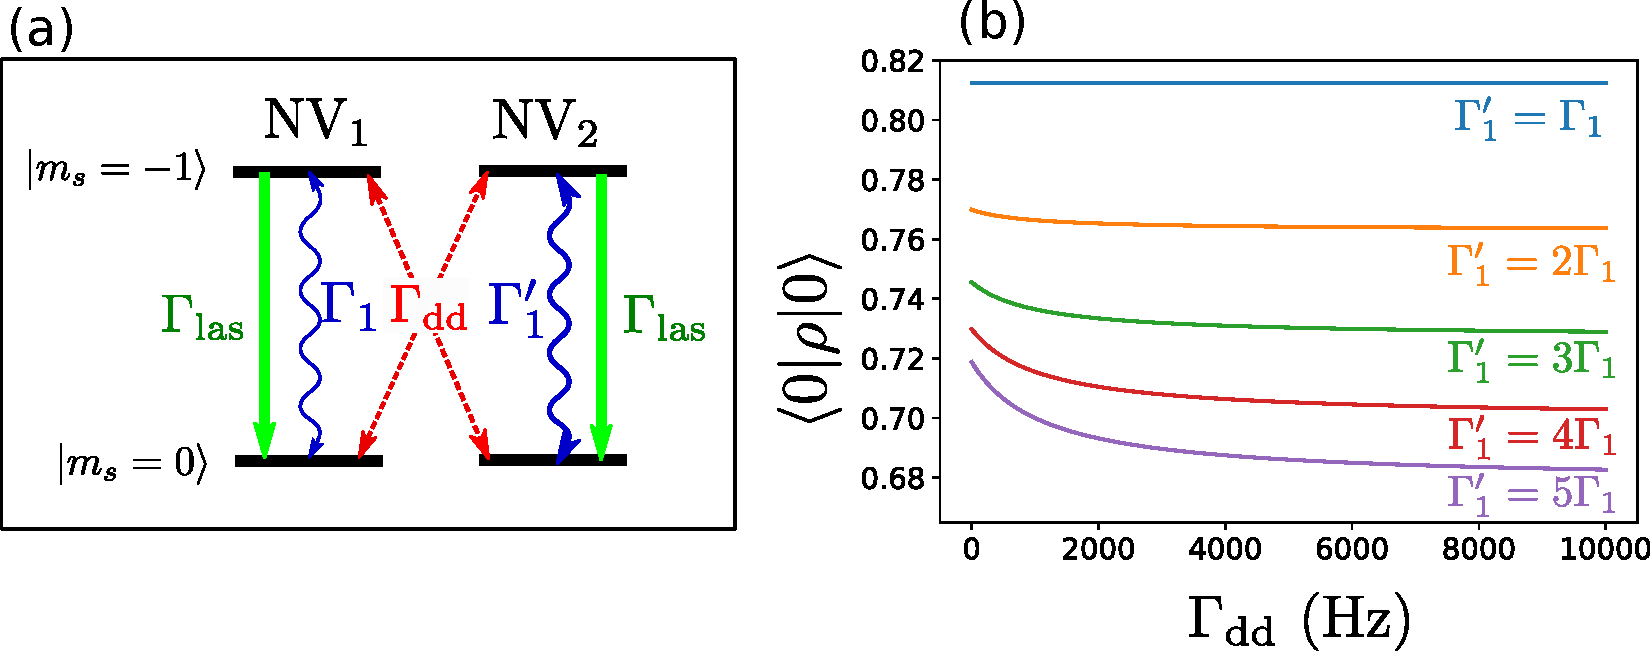
\includegraphics[width=\textwidth]{chapter 3/Figures/inhomogene_2_spins}
\caption{a) Schematics of the model: we consider a four level system consisting of 2 levels of 2 NV centers resonantly coupled through the flip-flop rate $\Gamma_{\rm dd}$. These two NV centers are each pumped in their respective $\ket{0}$ state via the green laser with a rate $\Gamma_{\rm las}$, and have their own relaxation rate $\Gamma_1$ and $\Gamma_1^*$ respectively. b) Average population of the two NV centers in the $\ket{0}$ state in the steady state as a function of $\Gamma_{\rm dd}$ and $\Gamma_1^*$. The steady state was computed by solving a classical rate equation where we fixed $\Gamma_{\rm las}=1000\ \rm Hz$ and $\Gamma_1=300\ \rm Hz$.}
\label{inhomogene}
\end{figure}
A likely explanation to the observed NV-NV CR is that the NV centers are not all equivalents.

Indeed, if we assume that, for instance, the relaxation rate $\Gamma_1=1/T_1$ is not strictly the same for each NV centers, but instead follows a certain distribution $\rho(\Gamma_1)$, then CR between NV centers with different $\Gamma_1$ can explain the observations in Fig. \ref{equivalent NV-NV}.

Fig. \ref{inhomogene}-a) and b) illustrates this case. Our model here consists of two (resonantly coupled) NV centers with two different relaxation rates $\Gamma_1$ and $\Gamma_1'$. To complete the model, we add the rate $\Gamma_{\rm las}$ which is the optical pumping rate from the $\ket{-1}$ to the $\ket{0}$ state of each spin, and $\Gamma_{\rm dd}$ the flip-flop rate between the two spins \footnote{We consider here a two level system instead of the full three levels of the spin 1. The choice of $\ket{-1}$ instead of $\ket{+1}$ is arbitrary.}. We only consider here the incoherent dynamics of the population, modeled with the rates reported on Fig. \ref{inhomogene}-a). Solving for the steady state of these rate equations, we can compute the final population in the $\ket{0}$ state for both spins. 

Fig. \ref{inhomogene}-b) shows the spin population in the $\ket{0}$ state of both spins, $\rho_{00}$, as a function of the flip-flop rate $\Gamma_{\rm dd}$ and for various values of $\Gamma_1'$. The first thing to notice is that, as $\Gamma_1'$ is increased,  $\rho_{00}$ decreases. This is because NV$_2$ becomes less polarized as its decay rate increases. The second thing to notice is that, when $\Gamma_1'=\Gamma_1$, i.e. when the two NV centers are truly equivalent, the flip-flop rate has no incidence on  $\rho_{00}$. However, when $\Gamma_1'>\Gamma_1$,  $\rho_{00}$ decreases when the flip-flop rate increases. Intuitively, this can be thought of as NV$_2$ acting as a polarization drain on NV$_1$. 

We can also notice that the influence of the flip-flop rate on $\rho_{00}$ increases when the difference in decay rates between NV$_1$ and NV$_2$ increases. As a result, we can suppose that a greater inhomogeneity between the NV centers would result in a stronger NV-NV cross-relaxation effect.


\subsection{Presentation of the fluctuator model}
\begin{figure}[h]
\centering
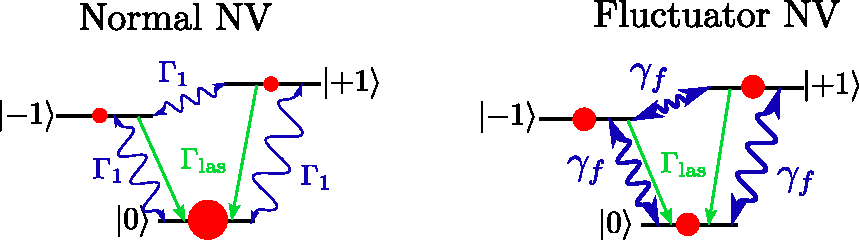
\includegraphics[width=.8\textwidth]{chapter 3/Figures/NV_vs_fluctuator}
\caption{Representation of a ``normal" NV center with spin depolarization rate $\Gamma_1 \ll \Gamma_{\rm las}$ and a fluctuator NV with spin depolarization rate $\gamma_f \gg \Gamma_{\rm las}$. Red circles represent the spin population in the steady state of each spin}
\label{NV vs fluct}
\end{figure}
Choi et al. in \citep{choi2017depolarization} take this approach a step further by separating the NV centers into two groups: ``normal" NV centers with a phonon-limited lifetime outside of dipole-dipole interaction, and ``fluctuators" which are NV centers with an intrinsic, extremely fast relaxation mechanism leading to a new depolarization rate $\gamma_f$. Normal and fluctuator NV are represented in Fig. \ref{NV vs fluct}: in their model, Choi et al. assume that the fluctuator decay rate is fast enough compared to the laser polarization rate $\gamma_f \gg \Gamma_{\rm las}$ that the fluctuators are effectively always depolarized. Fluctuators are therefore similar to the dark spins we introduced in the last chapter.

We should note here that, while this simplifications seem a bit extreme, the fluctuator model is more than a toy model. There are good evidence of the presence of these dark NV centers in dense NV ensemble, as will be discussed below.

In their model, the authors of \citep{choi2017depolarization} consider that the fluctuators act as a Markovian bath, meaning that the fluctuator density matrix will always read $\rho = \frac{1}{3} I$, regardless of its interaction with NV centers. With this assumption, the modification caused by the fluctuator bath on the ``normal" NV lifetimes can be analytically computed.

Other possibilities to explain the change in the relaxation rate were considered, such as spin diffusion to non-polarized NV centers (outside of the laser spot) or phonon superradiance, but they were not considered to be viable explanations: spin diffusion is orders of magnitude too slow to explain this phenomenon \citep{choi2017depolarization}, and the NV-NV CR seem to be independent of the crystal temperature \citep{jarmola2012temperature, mrozek2015longitudinal} which is incompatible with phonon superradiance \citep{choi2017depolarization}.

Before detailing the model's predictions, we will first contemplate the possible microscopic origin of these fluctuators, and review some physical systems were similar observations have been made.

 \subsection{Possible microscopic origin of the fluctuators}

We should note first that a similar problem of spin ensemble relaxation rate increasing with the spin concentration was observed more than six decades ago with phosphorus doped silicon \citep{feher1959electron,honig1960electron}. It was proposed that the cause of the relaxation was the presence of fast relaxing centers coupled to the slow relaxing centers through spin diffusion \citep{honig1960electron, sugihara1963spin, yang1968concentration, vugmeister1978spin, berman2005spin}. 

This conclusion was based on previous observations on the relaxation of nuclear spins \citep{bloembergen1949interaction, de1958relaxation, blumberg1960nuclear}, where some nuclear spins had a considerably reduced lifetime due to their proximity to paramagnetic ions. Similar observations were performed with Förster resonant energy transfer (FRET) in chromophore molecules \citep{forster1949experimentelle, eisenthal1964influence, yokota1967effects}, where excited donor molecules are coupled through (electric) dipole-dipole interaction to non-excited acceptor molecules.

In the case of P-doped Si, the origin of the fast relaxing centers is thought to be closely packed P impurities, so that the electronic wavefunctions of (at least) two P centers overlap. In that case two phenomena occur: the possibility of electron tunneling, and the apparition of a contact interaction term in the dipole-dipole Hamiltonian (cf eq. (\ref{eq. dipole quantique J coupling})). Both of these phenomena can lead to fast spin relaxation: electron tunneling can be accompanied by a spin reversal \citep{sugihara1963spin}, and the modulation of the contact interaction term ($J-$coupling) by the crystal phonons can directly excite the spin transitions \citep{honig1960electron}. While the dipole-dipole interaction terms (excluding the contact interaction) are also modulated by the phonons, this effect would be too small to account for the fast depolarization observed here.

Similarly, \citep{choi2017depolarization} suggests that the origin of fluctuators in NV centers are closely packed NV centers or NV-impurity pairs which undergo rapid electron hopping and spin depolarization. To prove their point, they look at the charge dynamics in their sample and find that there is charge recombination in the dark with a corresponding tunneling rate between neighboring sites of $\sim 10\ \rm ns$. In contrast to P-doped Si, the NV centers are not the most abundant electronic defects in the crystal, this is why the NV$^--$N$^+$ pair in particular is thought to be a likely candidate for the fluctuators \citep{manson2018nv}.

\subsection{Single NV center coupled to a single fluctuator}
We now turn to the computation of the depolarization induced by the fluctuator bath on the NV centers. We will follow here the notations and calculation steps in \citep{choi2017depolarization}. 

Let us first consider the interaction between a single NV center and a fluctuator. Since we assume the fluctuators to be always depolarized, this step is similar to the coupling of an NV center to a dark spin done in the last chapter.

We will first decompose the dipole-dipole Hamiltonian as a product between radial and angular part:
\begin{equation}
\mathcal{H}_{\rm dd} \approx - \frac{J_0}{r^3} \left[(g+ih)(\ket{0,+1}\bra{+1,0}+\ket{0,-1}\bra{-1,0}+qS_z^1 S_z^2 \right] + h.c. ,
\end{equation}
where the expression of $J_0, g, h$ and $q$ is given in appendix \ref{Appendix eta}. $g, h$ and $q$ are dimensionless factors that are function of the relative radial positions and orientation of the two dipoles.

We then introduce the dimensionless number $\eta$ defined as:
\begin{equation}
\label{eq eta}
\eta^2=\frac{1}{3} (\abs{g}^2+\abs{h}^2)  \frac{4\gamma_f^2}{(\omega_f - \omega_{NV})^2+4\gamma_f^2},
\end{equation}
where $\gamma_f$ is the fluctuator decay rate for each possible channel between $\ket{0}, \ket{-1}$ and $\ket{+1}$. This number $\eta$ encapsulates both the angular dependency (through $g$ and $h$) and the resonance condition between the NV center and the fluctuator.

We can note that the spectral response of a single fluctuator, for which we only consider the broadening caused by the decay rate $\gamma_f$, is a Lorentzian of half width $2\gamma_f$. This is different from the usual lifetime limited optical spectra which are Lorentzian of half width $1/2T_1=\Gamma_1/2$. The difference comes here from the fact that we consider thermalization going both ways (i.e. $\ket{e} \to \ket{g}$ and $\ket{g} \to \ket{e}$ instead of only $\ket{e} \to \ket{g}$) and that each state of the fluctuator can decay into two other states (see Fig. \ref{NV vs fluct}).

Finally, one finds that the additional depolarization rate induced by the fluctuator on the NV center reads:
\begin{equation}
\gamma_s(\mathbf{r})=\left(\frac{J_0}{r^3}\right)^2 \frac{\eta^2}{\gamma_f}.
\end{equation}
Compared to eq. (\ref{delta gamma 1}), the dependency on the inhomogeneous broadening of the spins $1/T_2^*$ is hidden in the $\eta$ factor, and we have the additional broadening $\gamma_f$ coming from the fluctuators very short lifetime.

\subsection{Ensemble of NV centers coupled to a bath of fluctuators}

\begin{figure}[h]
\centering
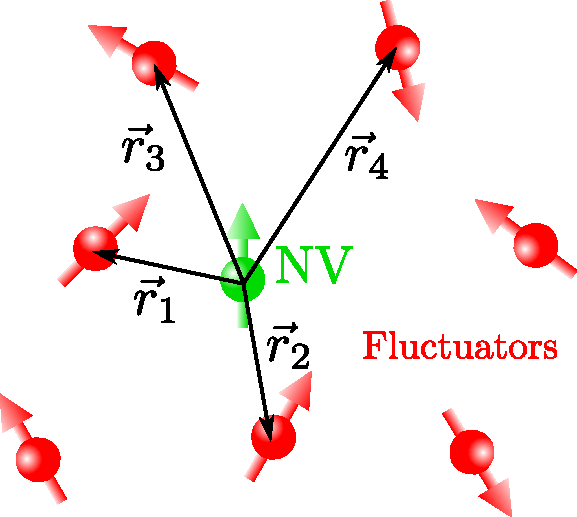
\includegraphics[width=.4\textwidth]{chapter 3/Figures/NV_dans_bain_fluct}
\caption{Schematics of an NV center in a fluctuator bath. The $\mathbf{r}_i$ vector represent the relative of position of fluctuator $i$ with respect to the NV center.}
\label{NV + bain fluct}
\end{figure}

The next step is to compute the depolarization caused by the ensemble of fluctuators on a single NV center.

We consider the situation pictured in Fig. \ref{NV + bain fluct}: the NV center is at the center of the frame and the position of each fluctuator is labeled $\mathbf{r}_i$. We consider that each fluctuator is an independent depolarization source, therefore the depolarization on a single NV center reads: 
\begin{equation}
\gamma=\sum_i \gamma_s(\mathbf{r}_i).
\end{equation}
We then want to compute the distribution $\rho(\gamma)$ defined as:
\begin{equation}
\rho(\gamma)=\int d\{r_i\} \rho(\{r_i\})\, \delta \left( \sum_i \gamma_s(\mathbf{r}_i) - \gamma \right).
\end{equation}
To do so, we need to determine the distribution of the fluctuators positions and orientations$\{r_i\}$. Assuming that they are homogeneously distributed in the bulk of the material, we find:
\begin{equation}
\rho(\gamma)=\frac{e^{-1/(4\gamma T)}}{\sqrt{4\pi \gamma^3 T}},
\end{equation}
where the time constant $T$ was introduced and is defined as:
\begin{equation}
\frac{1}{T}=\left(\frac{4\pi n_fJ_0\bar \eta}{3}\right)^2 \frac{\pi}{\gamma_f},
\label{eq 1/T}
\end{equation}
with $n$ the fluctuator density and $\bar \eta$ the averaged value of $\abs{\eta}$: 

\begin{equation}
\bar \eta = \int \rm{Prob}(\eta) \abs{\eta} d\eta.
\end{equation}

Finally, the polarization dynamics from the ensemble of NV centers can be computed:
\begin{equation}
P(t)=\int_0^\infty \rho(\gamma)\, e^{-\gamma t}d\gamma= e^{-\sqrt{t/T}}.
\end{equation}

In conclusion, the fluctuators causes a depolarization on the NV ensembles with a timsecale $T$ given by \ref{eq 1/T}, and the dynamics of this depolarization is that of a stretched exponential \footnote{Stretched exponential generally refer to functions of the form $\exp(-(t/\tau)^{\beta})$. In this manuscript, unless specified otherwise, we will always refer to the case $\beta=1/2$ when mentioning stretched exponential.}, unlike the phonon-induced depolarization which is purely exponential. 

It should be noted that the stretched exponential nature of the decay is not specific to the fluctuator model, but results from localized noise sources, randomly distributed in the bulk (3D). Indeed, \citep{hall2016detection} came to the same conclusion by analyzing the resonant coupling of NV centers with a P1 bath. Theodor Förster in 1949 also predicted and observed stretched exponential dynamics in the context of FRET, where the same scaling laws are observed \citep{forster1949experimentelle}.

\subsection{Computation of $\bar \eta$}
\label{sec computation eta}

The parameter $\bar \eta$ in eq. (\ref{eq 1/T}) is of crucial importance as it encapsulates the resonance condition between the NV centers and the fluctuators. This resonance condition, i.e. the spectral overlap between the fluctuators and the NV centers, can be decomposed in two essential parameters: one is the central frequency of each subgroup ($\omega_{NV}^0$ and $\omega_{f}^0$ respectively) which themselves depends on the magnetic field, the other is the spectral broadening of both the NV and the fluctuators. 

The aim of this section is to give an explicit formula of $\bar \eta$ as a function of $\omega_{NV}^0$, $\omega_{f}^0$ and $T_2^*$.

We will start by separating the factor $\eta$ given in eq. (\ref{eq eta}) into a a geometric and a spectral part:
\begin{align}
\eta^2&=G^2(\{\theta\}) R^2(\omega_f,\omega_{NV}), \\
G^2&=\frac{1}{3}\left(\abs{g}^2+\abs{h}^2 \right),  \\ 
R^2(\omega_f,\omega_{NV}) &= \frac{4\gamma_f^2}{(\omega_f - \omega_{NV})^2+4\gamma_f^2}.
\end{align}

$G$ is a function which depends purely on the various angles of the problem $\{\theta\}$, while $R$ represents the resonance condition between the NV and the fluctuator.

We then average the $\eta$ factor for an ensemble of fluctuators and NV centers:
\begin{align*}
\bar \eta &= \int \rm{Prob}(\eta) \abs{\eta} d\eta \\
&= \left(\int \rho(\{\theta\}) |G(\{\theta\})| d\{\theta\} \right) \\
&\, \times \left( \int \rho(\omega_{NV}) \rho(\omega_{f}) |R(\omega_f,\omega_{NV})| d\omega_{NV} d\omega_{f} \right) \\
&= \bar G \cdot \bar R,
\end{align*}
where we introduced $\rho(\{\theta\})$ the probability distribution of the angles $\{\theta\}$, $\rho(\omega_{NV})$ the inhomogeneous spectral distribution of the ensemble of NV centers and $\rho(\omega_{f})$ the inhomogeneous spectral distribution of the ensemble of fluctuators. We also introduced the notations $\bar G$ and $\bar R$ as the average of $|G|$ and $|R|$.

The computation of $\bar G$ will be further discussed in sec. \ref{sec quantitative T1} and in appendix \ref{delta gamma 1}. We will focus here on $\bar R$.

To perform the computation, we need to know the distributions $\rho(\omega_{NV})$ and $\rho(\omega_{f})$. We can experimentally measure $\rho(\omega_{NV})$ though ODMR, and we can reasonably expect $\rho(\omega_{f})$ to follow the same probability.

We unfortunately cannot analytically solve for $\bar R$ with standard distributions of $\rho(\omega_{f})$ and $\rho(\omega_{NV})$ (either Gaussians or Lorentzians). We can however solve for $\overline{R^2}$, which is close to $(\bar{R})^2$ as long as $2 \gamma_f \gg 1/T_2^*$.

For a Lorentzian profile of $\rho(\omega_{f})$ and $\rho(\omega_{NV})$ defined as:
\begin{align*}
\rho(\omega_{f})&=\frac{1}{\pi \Gamma_f} \frac{1}{1+ \left(\frac{\omega_f-\omega^0_f}{\Gamma_f}\right)^2} \\
\rho(\omega_{NV})&=\frac{1}{\pi \Gamma_{NV}} \frac{1}{1+ \left(\frac{\omega_{NV}-\omega^0_{NV}}{\Gamma_{NV}}\right)^2},
\end{align*}
where $\Gamma_{f}=1/T_2^*(\rm fluctuator)$ and $\Gamma_{NV}=1/T_2^*(\rm NV)$ are the inhomogeneous broadening of the NV and fluctuator ensembles, and $\omega^0_{NV}$ and $\omega^0_{f}$ are the central angular frequencies of the NV and fluctuator ensembles. We then find that:

\begin{align*}
\overline{R^2}&= \int \rho(\omega_{NV}) \rho(\omega_{f}) \frac{4\gamma_f^2}{(\omega_f - \omega_{NV})^2+4\gamma_f^2} d\omega_{NV} d\omega_{f} \\
&=\frac{2 \gamma_f}{2 \gamma_f + \Gamma_f + \Gamma_{NV}} \cdot \frac{1}{1+\left(\frac{\omega^0_{NV}-\omega^0_{f}}{2 \gamma_f + \Gamma_f + \Gamma_{NV}}\right)^2}.
\end{align*}

In the case where $\omega^0_{NV}=\omega^0_{f}$, meaning that either the considered NVs and fluctuators are from the same class, or from two classes perfectly resonant, by substituting $\overline{R ^2}$ for $(\bar{R})^2$ (which again is only approximately valid for $2 \gamma_f \gg 1/T_2^*$) in eq. \ref{eq 1/T}, we find that:
\begin{equation}
\label{eq 1/T avec T2*}
\frac{1}{T} \propto \frac{1}{2\gamma_f + \Gamma_f + \Gamma_{NV}}\cdot \frac{1}{1+\left(\frac{\omega^0_{NV}-\omega^0_{f}}{2 \gamma_f + \Gamma_f + \Gamma_{NV}}\right)^2}.
\end{equation}

If $\rho(\omega_{f})$ and $\rho(\omega_{NV})$ follow Gaussian profiles instead, $\overline{R^2}$ is the integral of a Voigt profile, the convolution of a Lorentzian and a Gaussian, which does not have a clear analytic solution.

Eq. \ref{eq 1/T avec T2*} was obtained via several approximations: the inhomogeneous distribution of the NV centers is generally not Lorentzian, and $\overline{R^2} \neq (\bar{R})^2$ in the general case. Nevertheless, it gives us a general idea of the evolution of $1/T$ with $T_2^*$, $\omega_{NV}^0$ and $\omega_{f}^0$, which will be crucial to compare the predictions of the model with experimental data.






\section{Experimental investigation of the fluctuator model}
We will now show experimental results related to the predictions of the fluctuator model.
\subsection{The stretched exponential lifetime}
\begin{figure}[h]
\centering
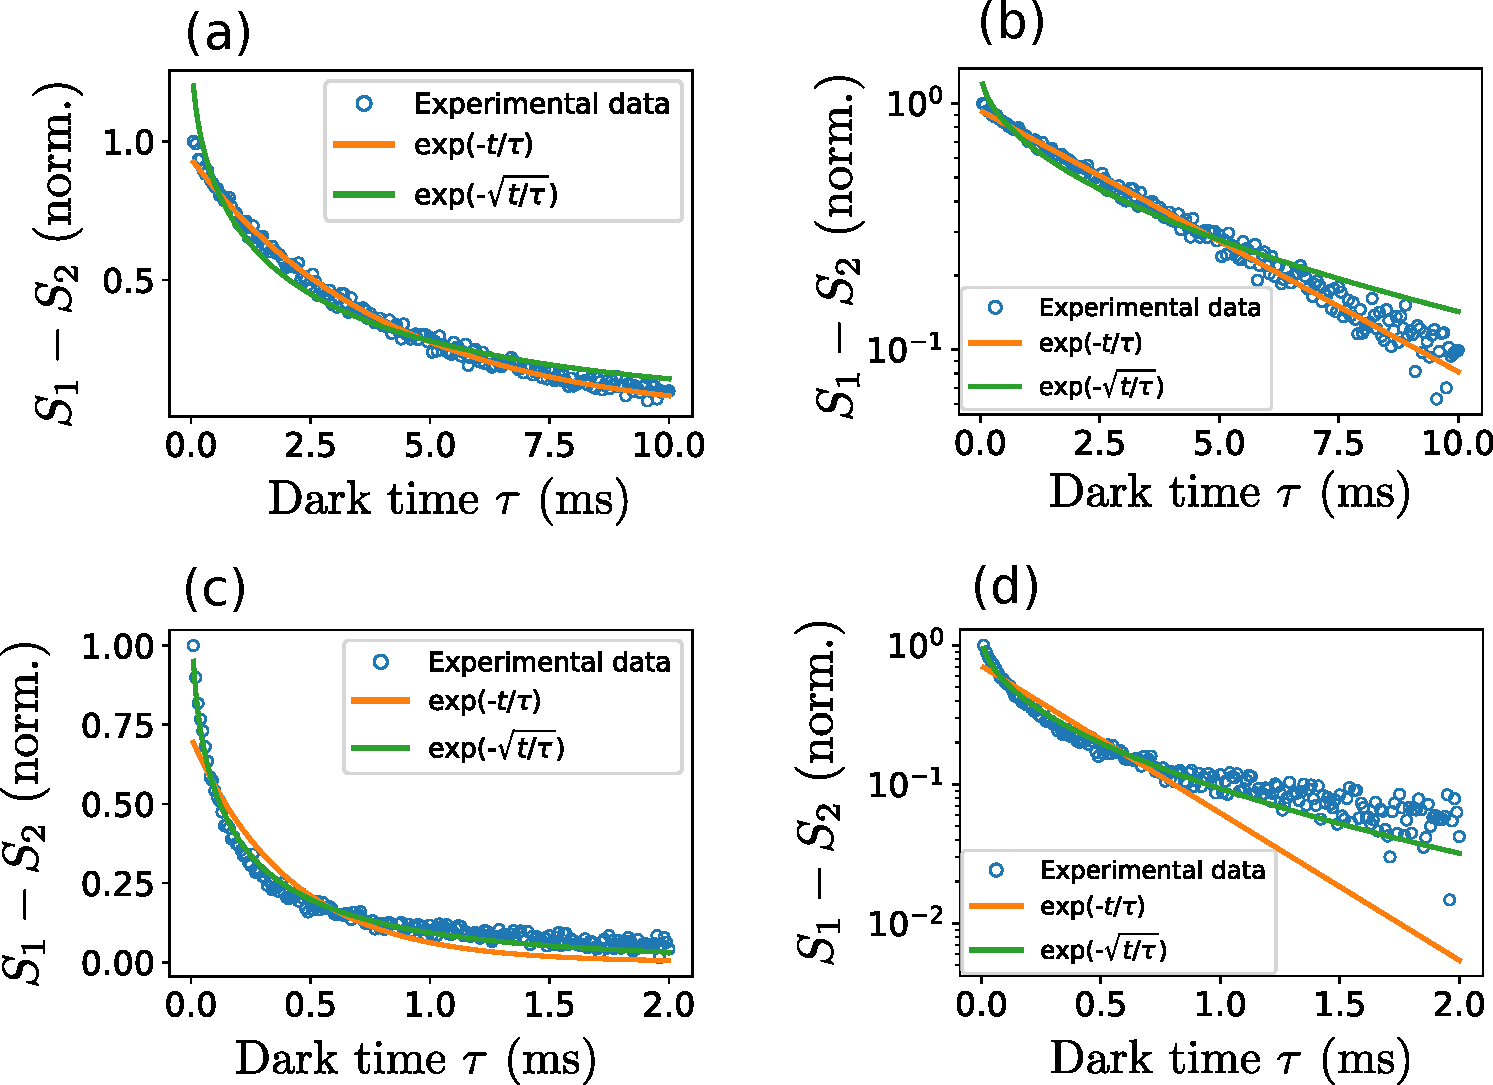
\includegraphics[width=\textwidth]{chapter 3/Figures/Stretch_vs_pas_stretch}
\caption{T1 measurement following the protocol described in Fig. \ref{T1 soustraction}. The best exponential and stretched exponential fits are given in every case. a) Sample CVD-pink with B$\neq$0 and a single  probed class. The optimal $T_1$ values are $T_1^{\rm stretch}=1.9\ \rm ms$ and $T_1^{\rm exp}=4.1\ \rm ms$. b) Same measurement as a) in log scale. c) Sample ADM-15-2 with B=0. The optimal $T_1$ values are $T_1^{\rm stretch}=150\ \mu \rm s$ and $T_1^{\rm exp}=410\ \mu \rm s$. d) Same measurement as c) in log scale.}
\label{stretch_or_not_stretch}
\end{figure}

The first prediction of the fluctuator model which can be experimentally verified is the stretched-exponential profile of the spin relaxation. The protocol to measure spin relaxation with a common mode rejection was presented in Fig. \ref{T1 soustraction}. 

Fig. \ref{stretch_or_not_stretch} shows the results of this protocol on two distinct samples and magnetic field configurations. In both cases, we show the results in linear and logarithmic scale as the log scale makes deviations from the standard exponential more apparent\footnote{The fits presented in Fig. \ref{stretch_or_not_stretch} and in the next figures were performed by fitting the real value of $S_1-S_2$ and not $\log(S_1-S_2)$.}.

The spin relaxation results presented in Fig. \ref{stretch_or_not_stretch}-a) and b) was performed on sample CVD-pink (see sample details in appendix \ref{Appendix samples}), which despite a relatively high NV concentration shows only moderate amount of dipole-dipole spin relaxation. In order to further minimize the amount of cross-relaxations, we chose a magnetic field for which all four NV classes are spectrally isolated, so that only fluctuators from the same class as the NV center could lead to relaxation. As a result, we can see a relaxation profile mostly exponential with a lifetime $T_1=4.1\ \rm ms$ comparable to the phonon-limited $T_1$ value of $\sim 5\ \rm ms$ at room temperature \citep{jarmola2012temperature}.

The second spin relaxation presented in Fig. \ref{stretch_or_not_stretch}-c) and d) was performed on sample ADM-15-2 which showed a great amount of dipole-dipole spin relaxation. To further enhance the cross-relaxation rate, the experiment was performed in zero external magnetic field so that every class of NV centers would be resonant. We can observe a relaxation profile that deviates significantly from tthe exponential profile, and which is nicely fitted by a stretched exponential. The $T_1$ value obtained from the fit is also an order of magnetite lower than the phonon-limited value, which is coherent with the fact that dipole-dipole interactions dominate the spin relaxation in this case.

\subsection{Fitting $T_1$ profile in the general case}

\begin{figure}[h]
\centering
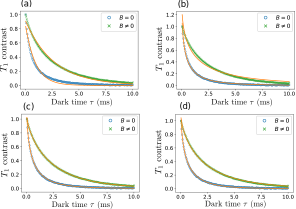
\includegraphics[width=\textwidth]{chapter 3/Figures/various_fit_formulae}
\caption{Different fitting procedure on two $T_1$ measurements done on sample ADM-150-1 for $B=0$ and $B\neq0$. \\ a) Exponential fit $S(\tau)=\exp (-\tau/T_1^{\rm ph})$. \\ b) Stretched exponential fit $S(\tau)=\exp (-\sqrt{\tau/T_1^{\rm dd}})$. \\ c) Bi-exponential fit $S(\tau)=\exp (-\tau/T_1^{\rm ph} -\sqrt{\tau/T_1^{\rm dd}})$. \\ d) Bi-exponential fit with fixed $T_1^{\rm ph}=5\ \rm ms$: $S(\tau)=\exp (-\tau/5 -\sqrt{\tau/T_1^{\rm dd}})$.}
\label{various_fit_formulae}
\end{figure}

\begin{table}[htbp]
\centering
\caption{Fitting parameters for Fig.
 \ref{various_fit_formulae}. The coefficient of determination $R^2$ for each fit is reported here.}
 \label{fitting table}
\begin{tabular}{c|ccc|ccc}
\toprule
Figure &  \multicolumn{3}{c}{$B=0$} & \multicolumn{3}{c}{$B\neq0$}\\
\midrule
{} &  $T_1^{\rm ph}$ (ms)& $T_1^{\rm dd}$ (ms) & $1-R^2$ &  $T_1^{\rm ph}$ (ms)& $T_1^{\rm dd}$(ms)& $1-R^2$\\
\midrule
Fig. a) & 0.95 & * & $2\cdot 10^{-2}$ & 2.64 & * & $6\cdot 10^{-3}$ \\
Fig. b) & * & 0.32 & $2\cdot 10^{-3}$& * & 1.03 & $2\cdot 10^{-2}$ \\
Fig. c) & 6.75 & 0.44 & $6\cdot 10^{-4}$ & 4.22 & 7.19 & $2\cdot 10^{-4}$\\
Fig. d) & \textbf{5} & 0.51 & $6\cdot 10^{-4}$ & \textbf{5} & 4.65 & $6\cdot 10^{-4}$\\
\bottomrule
\end{tabular}

Bold characters indicate parameters that were arbitrarily fixed.
\end{table}

For many samples, the $T_1$ profile is neither fully exponential nor fully stretched exponential, because the relaxation time associated with CR, which we will call $T_1^{\rm dd}$, is of the same order of magnitude as the phonon limited lifetime $T_1^{\rm ph}$. Sometimes the same sample can go from mostly exponential to mostly stretched exponential depending on the number of NV-NV co-resonances, meaning that we have to include both aspects in the fitting formula.

Fig. \ref{various_fit_formulae} shows four different fitting procedure on the two same relaxation measurements. The measurements were performed on the same sample ADM-150-1, with and without an external magnetic field ($\sim 50 G$). The magnetic field was strong enough to split the four classes and only one class was probed in the case $B\neq0$ , whereas all 4 classes were resonant in the case $B=0$, which strongly increases the NV-NV CR. 

The fits used here are either purely exponential or purely stretched exponential, or a combination of both where the exponential lifetime $T_1^{\rm ph}$ was either left as a free parameter or fixed at a value $T_1^{\rm ph}=5\ \rm ms$. The values of the different fitting parameters used is reported in Table \ref{fitting table}.

We can see that neither the purely exponential nor stretched exponential fits can be satisfying for both measurements: the $B=0$ curve is poorly fitted by the exponential fit and the $B \neq 0$ curve is poorly fitted by the stretched exponential. The protocols that include both exponential and stretched lifetimes correctly fit both curves. In the case of Fig. \ref{various_fit_formulae}-d), we arbitrarily fixed $T_1^{\rm ph}=5\ \rm ms$ since this is the value we typically measure on samples with low NV density, and we expect that the phonon-limited exponential lifetime is not modified by the NV concentration.

Both the protocol where $T_1^{\rm ph}$ was fixed and the one where it was not correctly fit our data. We therefore decided to use the protocol where $T_1^{\rm ph}$ was fixed in order to minimize the number of free parameter in the fitting function. This way, the values of $T_1^{\rm dd}$ obtained on different measurements can be directly compared. 

We should note however that the values of $T_1^{\rm dd}$ we obtain are not absolute. Indeed, in the case of Fig. \ref{various_fit_formulae}, the value of $T_1^{\rm ph}$ can be somewhat arbitrarily fixed between 3 and 6 ms with satisfying fits, and the resulting values $T_1^{\rm dd}$ can vary by almost an order of magnitude in the case of $B\neq0$. The values of $T_1^{\rm dd}$ obtained with this method have therefore to be be compared to values from the same method and the same fixed value of $T_1^{\rm ph}$.

\begin{figure}[h]
\centering
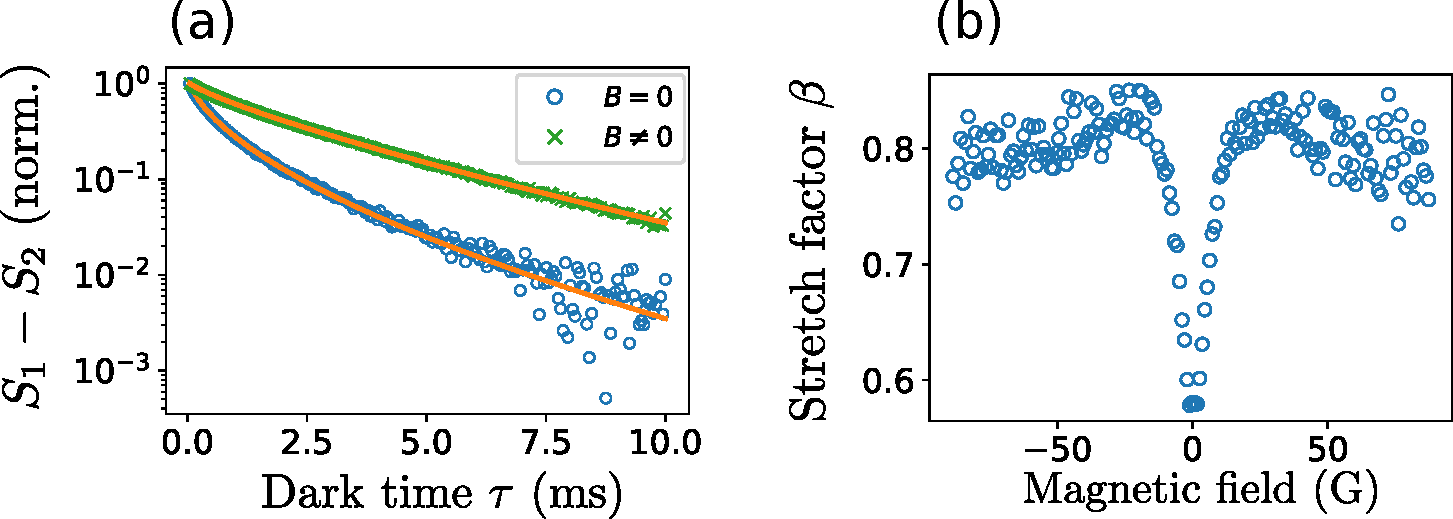
\includegraphics[width=\textwidth]{chapter 3/Figures/betas}
\caption{a) Same two measurements as Fig. \ref{various_fit_formulae} with the fitting formula $S(\tau)=\exp ((-\tau/T_1)^{\beta})$. The fitting parameters are $\beta=0.58$ and $T_1=0.46\ \rm ms$ for $B=0$, and $\beta=0.80$ and $T_1=2.15\ \rm ms$ for $B\neq0$. b) Optimal $\beta$ parameter found for each $T_1$ measurement as a function of the external magnetic field (still on sample ADM-150-1).}
\label{betas}
\end{figure}

Finally, another fitting procedure is shown in Fig. \ref{betas}. This time a single stretched exponential with an arbitrary stretch factor $\beta$ is used, and satisfyingly fits the data. Fig. \ref{betas}-b) shows the optimal $\beta$ parameter as a function of the external magnetic field. It confirms that the $T_1$ profile gets closer to a stretched exponential ($\beta=0.5$) when $B$ goes to 0. Even though this method also yields satisfying fits, it employs more free parameters ($\beta$ and $T_1$) than the method of \ref{various_fit_formulae}-d). We therefore decided to go with the later.

\subsection{The fluctuators linewidth}

\subsubsection{The fluctuators spectral response}
\begin{figure}[h]
\centering
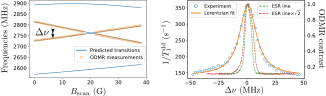
\includegraphics[width=\textwidth]{chapter 3/Figures/fluctuator linewidth}
\caption{Measurement of the fluctuators linewidth on sample ADM-150-2 using the same setup as in Fig. \ref{equivalent NV-NV}. a) Simulation of the $\ket{0} \to \ket{-1}$ transition frequency for the four classes of NV centers and actual frequencies of the two central classes from ODMR measurements. b) Measurement of $T_1^{\rm dd}$ as a function of the splitting $\Delta \nu$ between the two central classes, fitted with a Lorentzian of half-width $\sigma=8.8 \pm 0.2\ \rm MHz$. The green dashed line correspond to the ODMR spectrum of a single class of NV centers, and the red dashed one to the same line scaled up by a factor of 2}
\label{fluct linewidth}
\end{figure}

We now move to the second major prediction of the fluctuator model which is the spectral broadening of the fluctuators caused by the their relaxation rate $\gamma_f$. Indeed, following the arguments presented in \citep{choi2017depolarization}, the fluctuators homogeneous spectral response is a Lorentzian of half-width $2\gamma_f$. The inhomogeneous spectral response of the ensemble of fluctuators is then further broadened by the same electric, magnetic or strain noises than the NV centers, which is characterized by $1/T_2^*$.

The fluctuator are effectively dark to ODMR measurement since they are not polarized, meaning that we cannot directly measure their linewidth as we would do for normal NV centers. We can however measure their linewidth through cross-relaxation, similarly to the detection of dark spins presented in the previous chapter.

Fig. \ref{fluct linewidth} shows an experiment similar to the one presented in Fig. \ref{equivalent NV-NV}. A variable magnetic $B_{\rm scan}$ in addition to an offset magnetic field $B_{\rm DC} \sim 100\ \rm G$ are used in order to create a crossing between two classes of NV centers. This time however, the spin relaxation was measured instead of the PL.

Fig. \ref{fluct linewidth}-a) shows the simulated transitions of the four classes of NV centers as a function of the magnetic field. We took particular care in measuring the central frequencies of the two classes of interest (when the two lines could be clearly separated), since having a precise measurement of the detuning between the two classes $\Delta \nu$ is key to get a precise value of the fluctuator linewidth.


Fig. \ref{fluct linewidth}-b) shows the dipole-dipole induced relaxation rate $\Gamma_1^{\rm dd}=1/T_1^{\rm dd}$ as a function of the detuning $\Delta \nu$ between the two central classes. For each magnetic field value, a $T_1$ profile was recorded and fitted following the procedure described in Fig. \ref{various_fit_formulae}-d) where we again fixed $T_1^{\rm ph}=5\ \rm ms$. We also show the ODMR spectrum of a single NV class for comparison.

We can clearly see that the $\Gamma^{\rm dd}$ profile is much broader than the ODMR line of the NV centers, whereas in a standard CR process, we expect the decay rate to be proportional to the spectral overlap of the two classes \citep{hall2016detection}. If we assume that both NV classes spectral response are Lorentzian of same width $\sigma$, then the spectral overlap between the two classes is also a Lorentzian of width $2 \sigma$ \footnote{For other line profile, the overlap would be smaller than $2 \sigma$. For instances, the overlap of two Gaussians of width $\sigma$ is a Gaussian of width $\sqrt{2} \sigma$}. Fig. \ref{fluct linewidth}-b) also shows the ODMR line scaled by a factor $2$, which is still significantly narrower than the $1/T_1^{\rm dd}$ line.

We attribute this broadening to the fluctuators lifetime. Another potential explanation for the broadening could be the interaction strength between the NV center and the fluctuator, but for [NV] $\sim$ 5 ppm, the average dipole-dipole coupling strength between closest NV neighbor is $\expval{\mathcal{H}_{\rm dd}} \sim 46\ \rm kHz$, which cannot explain the $\sim 4\ \rm MHz$ broadening observed here.

\subsubsection{The fluctuators lifetime}
\label{sec fluctuators lifetime}
\begin{figure}[h]
\centering
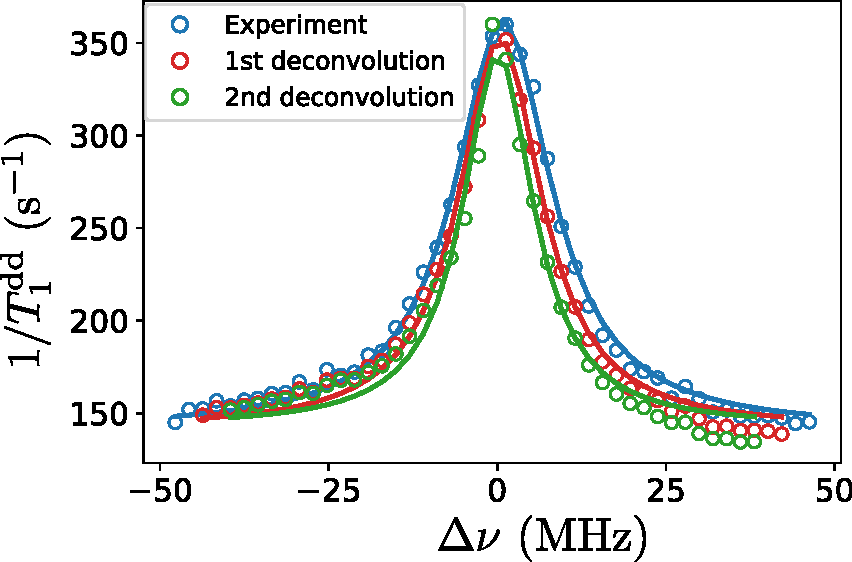
\includegraphics[width=0.6\textwidth]{chapter 3/Figures/deconvolution}
\caption{Blue curve $1/T_1^{\rm dd}$ data presented in Fig. \ref{fluct linewidth}. Red curve: deconvolution of the blue curve by the ODMR line shown on the same figure. Green curve: deconvolution of the red curve   by the ODMR line. All three curves are fitted with Lorentzian of respective half widths $8.8 \pm 0.2$, $7.5 \pm 0.3$ and $6.4 \pm 0.4$ MHz (the precision is determined by the variance of the optimal fit parameters)}
\label{deconvolution}
\end{figure}

We now want to extract the fluctuators lifetime $T_1^f=1/\gamma_f$ to get further information on their potential nature. 

To do this we first assume that the dipole induced decay rate is proportional to the overlap of the spectral responses of the NV centers and fluctuators $S_{NV}$ and $S_f$. We will take $S_{NV}( \omega)$ and $S_{f}( \omega)$ as functions centered in $\omega=0$, and consider that the spectral responses are shifted by $\omega^0_{NV}$ and $\omega^0_{f}$ respectively, the central frequencies of each group. We then have:
\begin{align*}
\frac{1}{T_1^{\rm dd}} &\propto \int S_{NV} (\omega-\omega_{NV}^0) S_f (\omega-\omega_{f}^0) d\omega \\
&= \int S_{NV} (\omega-\Delta \omega) S_f (\omega)
 d\omega \\
 &= (S_{NV}*S_{f})(\Delta \omega),
\end{align*}

where $\Delta \omega=\omega_{NV}^0-\omega_{f}^0$.

Using the approximation $\bar {R ^2} \approx (\bar{R})^2$ detailed in sec. \ref{sec computation eta}, we can then decompose the fluctuator spectral response as a convolution of the lifetime contribution and the inhomogeneous broadening:
\begin{equation}
S_{f}(\omega)=\left(S_f^*(\omega)\right)*\left(\frac{1}{1+\left(\frac{\omega}{2 \gamma_f}\right)^2} \right),
\end{equation}

where $S_f^*$ is the spectral broadening caused by the inhomogeneous distribution of the fluctuators, which we will suppose to be equal to $S_{NV}$. With these assumptions, we are now ready to extract $\gamma_f$ from the data of Fig. \ref{fluct linewidth}.

The first way to do this, as was done for NV-P1 CR in \citep{hall2016detection}, is to deconvolve the $1/T_1^{\rm dd}$ data by the ODMR spectrum using a Wiener deconvolution algorithm. The result of the deconvolution is shown in Fig. \ref{deconvolution}: the data is deconvolved once to get the spectral response of the fluctuator (red curve), and a second time to get only the lifetime contribution of the fluctuator (green curve). Fitting with Lorentzians, we find a final value $\Gamma_2 =2\gamma_f= (2\pi) 6.4 \pm 0.4\ \rm MHz$ which corresponds to a fluctuator lifetime $T_1^f=\frac{1}{\gamma_f}=50 \pm 3\ \rm ns$\footnote{We define here the fluctuators lifetime $T_1^f$ as $\frac{1}{\gamma_f}$ for simplicity, but it should be noted that the actual lifetime of the fluctuators states is $\frac{1}{2\gamma_f}$ due to the competition between the two possible decay channels for each state (cf Fig. \ref{NV vs fluct}).}.

Another, simpler alternative is to consider that the $1/T_1^{\rm dd}$ profile is a Voigt profile given by the convolution of two Gaussians of half width at half maximum (HWHM) $f_G=\frac{\sqrt{\ln (2)}}{\pi T_2^*}$ and a Lorentzian of HWHM $f_L=\frac{2 \gamma_f}{2 \pi}$:
\begin{align*}
\Gamma_1^{\rm dd}&\propto \mathcal{G}(f_G)*(\mathcal{L}(f_L)*\mathcal{G}(f_G)) \\
&\propto \mathcal{L}(f_L)*\mathcal{G}(\sqrt{2} f_G),
\end{align*}
where $\mathcal{G}(f_G)$ and $\mathcal{L}(f_L)$ denote Gaussian and Lorentzian functions of HWHM $f_G$ and $f_L$ respectively.
We can then use the formula of a pseudo-Voigt profile which gives an approximation of the Voigt profile's HWHM $f$ as a function of $f_G$ and $f_L$ \citep{ida2000extended}:
\begin{equation}
f = [f_G^5 + 2.69269 f_G^4 f_L + 2.42843 f_G^3 f_L^2 + 4.47163 f_G^2 f_L^3 + 0.07842 f_G f_L^4 + f_L^5]^{1/5}.
\end{equation}

With $f=8.8 \pm 0.2\ \rm MHz$ and $\sqrt{2}f_G=4.3 \pm 0.2\ \rm MHz$, we find $f_L=6.5 \pm 0.3\ \rm MHz$ for a final lifetime value $T_1^f = 49 \pm 2\ \rm ns$, a value consistent with the one found with the deconvolution method.

Doing similar experiments and calculations, \citep{choi2017depolarization} found $\gamma_f=1/T_1^f=(2\pi) 3.3\ \rm MHz$ which gives them a fluctuator lifetime value $T_1^f = 48\ \rm ns$, a value very close to the ones we obtained above, despite using a completely different sample.

In conclusion, we observed that the fluctuators linewidth was indeed broadened by their relaxation rate which justifies the initial hypothesis that $T_1^f \ll T_1^{NV}$. It even shows that $T_1^f$ is of the same order of magnitude as the optical lifetime ($\sim 15\ \rm ns$) which explains why the fluctuators cannot be optically polarized.

\section{Resonance between several NV classes}

The main tool to probe NV-NV CR is to use the co-resonances between the NV classes. While it is not possible to completely shut down the CR, because the NV centers from the same class are always resonant with each other, we can tune the density of resonant NV centers (and resonant fluctuators) by a factor of 4 by playing with the inter-class co-resonances. In this section, we will discuss the various scenarios where NV classes overlap, and quantify theoretically and experimentally the dipole-induced relaxation rate in each case.

\subsection{Geometric conditions for inter-class resonance}
\label{sec geometrie resonance}

\begin{figure}[h!]
\centering
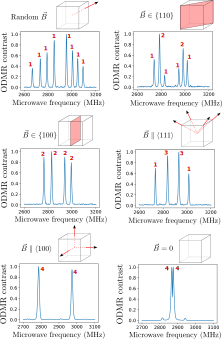
\includegraphics[width=0.8\textwidth]{chapter 3/Figures/Resonance_geometries}
\caption{ODMR spectra on sample ADM-15-3 as a function of the magnetic field orientation. The field amplitude is $\sim 60\ \rm G$. Red numbers represent the number of resonant classes for each ODMR line. The cubes represent the diamond unit cell, and the red planes/arrow the possible orientations of the magnetic field}
\label{ODMR_geometries}
\end{figure}

There are four possibilities to obtain inter-class resonance (aside from the non-equivalent CR discussed in sec. \ref{non_equi_valent_CR}). These possibilities are:
\begin{itemize}
\item $\mathbf{B} \in \{110\}$. We refer by $\{110\}$ as any plane orthogonal to a $\langle 110 \rangle$ or equivalent direction. In this magnetic configuration, two classes are at resonance and the two other ones are spectrally isolated.
\item $\mathbf{B} \in \{100\}$. In this magnetic configuration, the four classes form two pairs of co-resonance.
\item $\mathbf{B} \parallel \langle 111 \rangle$. In this configuration discussed in the last chapter, one class is aligned with the magnetic field and is spectrally isolated while the three other form a resonant triplet.
\item $\mathbf{B} \parallel \langle 100 \rangle$. In this configuration also discussed in the last chapter, the four classes are resonant.
\end{itemize}
We should add to this list the case $\mathbf{B}=0$ where all four classes are also resonant, and any other possibility (which we will label random $\mathbf{B}$) where all four classes are spectrally separated. 

An ODMR spectrum and a representation of the magnetic field in the diamond unit cell for each of these six possibilities is shown in Fig. \ref{ODMR_geometries}.

\begin{figure}[h]
\centering
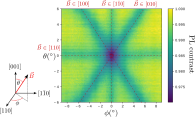
\includegraphics[width=\textwidth]{chapter 3/Figures/carte}
\caption{PL contrast as a function of the magnetic field polar and azimuthal angle with respect to the [100] axis on sample CVD-pink. The field amplitude is $\abs{B} \sim 115 G$. The locus of the magnetic field in specific planes is noted by red dashed lines.}
\label{Carte}
\end{figure}

This relation between NV-NV class resonances and the magnetic field being in specific crystalline planes or directions means that we can determine the crystal main axes simply by PL experiments.

Fig. \ref{Carte} shows a map where we monitored the PL of sample CVD-pink while scanning the magnetic field angle around the [001] axis, thanks to a permanent magnet on a motorized goniometer. We have also reported the locus of $\mathbf{B}$ being in the planes [100], [010], [110] and [$1\bar 1 0$].

We know that when $\mathbf{B}$ belongs to any of these four planes, there is a co-resonance between at least two NV classes. This co-resonance leads to an increase in NV-NV CR and a faster depolarization of the spins involved, which ultimately leads to a drop in PL. We can indeed see in fig. \ref{Carte} that there is clear correlation between the loci of $\mathbf{B}$ and drops in PL. We can also see that the PL is at its lowest when $\mathbf{B}\parallel [001]$, which corresponds to a four class degeneracy.

\subsection{Quantitative modification of $T_1$}
\label{sec quantitative T1}
\begin{table}[htbp]
\centering
\caption{Theoretical and experimental values of $\Gamma_1^{\rm dd}=1/T_1^{\rm dd}$ for various magnetic field configurations, expressed as a function of the value found for an isolated class. The experimental values were measured on sample ADM-15-3 using the protocol of Fig. \ref{various_fit_formulae}-d) with $T_1^{\rm ph}= 5\ \rm ms$. The uncertainty corresponds to the precision of the fit parameters.}
 \label{T1 champ mag}
\begin{tabular}{c|cc}
\toprule
$\Gamma_1^{\rm dd} (\mathbf{B})$ &  Theory & Experimental \\
\midrule
random $\mathbf{B}$ (1 class) & $\Gamma_0^{\rm th}$ & $1.53\pm 0.04$ ms$^{-1} \equiv \Gamma_0^{\rm exp}$ \\
$\mathbf{B} \in \{110\}$ (2 classes) & 10.0 $\Gamma_0^{\rm th}$ & $5.2 \pm 0.1$ $\Gamma_0^{\rm exp}$ \\
$\mathbf{B} \in \{100\}$ (2 classes) & 7.24 $\Gamma_0^{\rm th}$ & $4.2 \pm 0.1$ $\Gamma_0^{\rm exp}$ \\
$\mathbf{B} \parallel \langle 111 \rangle$ (3 classes) & 28.4 $\Gamma_0^{\rm th}$ & $11.6 \pm 0.4$ $\Gamma_0^{\rm exp}$ \\
$\mathbf{B} \parallel \langle 100 \rangle$ (4 classes) & 42.8 $\Gamma_0^{\rm th}$ & $14.1 \pm 0.5$ $\Gamma_0^{\rm exp}$ \\
$\mathbf{B}=0$ (4 classes) & 51+($^*$) $\Gamma_0^{\rm th}$ & $19.9 \pm 0.8$ $\Gamma_0^{\rm exp}$ \\
\bottomrule
\end{tabular}

($^*$) The case $\mathbf{B}=0$ will be detailed in the next chapter. The theoretical value is a lower bond.
\end{table}

The fluctuator model allows quantitative predictions of the change in the spin lifetime, thanks to eq. \ref{eq 1/T}. There are however several unknowns in this equation, such as the fluctuator density and lifetime which can be hard to estimate. It is however relatively easy to compare the predictions of eq. \ref{eq 1/T} for various magnetic field configurations.

We decided to take the case of an isolated class as the baseline value for the dipole-dipole decay rate $\Gamma_0$, and to express the decay rates when 2, 3 or 4 classes are co-resonant as a function of $\Gamma_0$. Doing so allows us to normalize $n_f$ and $\gamma_f$ in eq. \ref{eq 1/T} and to keep $\bar G$ the geometrical part of $\bar \eta$ as the only unknown.

$\bar G$ can be analytically or numerically computed for each of the magnetic configurations listed before, as detailed in appendix \ref{Appendix eta}. This allows us to predict the value of the spin decay rate in every situations as a function of the decay rate of an isolated class.

Table \ref{T1 champ mag} shows these predicted values, along with experimental ones on sample ADM-15-3. The experimental values were obtained with the protocol described in Fig. \ref{various_fit_formulae}-d) with a double exponential fit where we fixed again $T_1^{\rm dd}=5\ \rm ms$.

The theoretical values are in a good qualitative agreement with the experimental ones, both ranking the different scenarios in the same order. The quantitative predictions of the theory however are rather poor, being off by more than a factor of 3 for the shortest lifetimes.

It should be noted that the experimental values were heavily influenced by the choice of the parameter $T_1^{\rm ph}$. Using for example $T_1^{\rm ph}=2.5\ \rm ms$ gave results closer to the theoretical ones. Nevertheless, the fluctuator model generally tends to overestimate the depolarization rates.The authors of \citep{choi2017depolarization} for instance found that a 2-class degeneracy (the authors did not precise whether this was a $\mathbf{B} \in \{110\}$ or $\mathbf{B} \in \{100\}$ configuration) yielded an increased depolarization rate by a factor $\sim 4$, a value comparable to the one we found in table \ref{T1 champ mag}, and two times smaller than the predicted one\footnote{We can also see in Fig. \ref{fluct linewidth} that a $\mathbf{B} \in \{110\}$ configuration leads to a $\sim 2.5$ times increase in $\Gamma_1^{\rm dd}$, which is 4 times smaller than the predicted factor of 10.}.

The failure of the fluctuator model to accurately predict the changes in $T_1$ is one of the reasons that led us to believe that the model is incomplete. Other reasons will be presented in the following part.

\section{Conclusion and perspectives}

In conclusion, we have seen in this chapter that dense NV ensemble present ``anormal" CR between the NV centers, and we have shown how the fluctuator model developed by Choi et al. in \citep{choi2017depolarization} can explain this behavior. The fluctuator model not only explains the NV-NV CR, but also correctly predicts the stretched exponential lifetime profile. It also correctly predicts that the fluctuators have a broader spectral response than the other NV centers. Nevertheless, the model does not describe perfectly every aspects of NV-NV relaxation, and there still are many aspects of this problem, both theoretical and experimental, to explore.

In what follows we will describe what could be interesting investigation points to further understand the NV-NV relaxation and the fluctuator model.

\subsection{Limitations of the fluctuator model}
\begin{figure}[h]
\centering
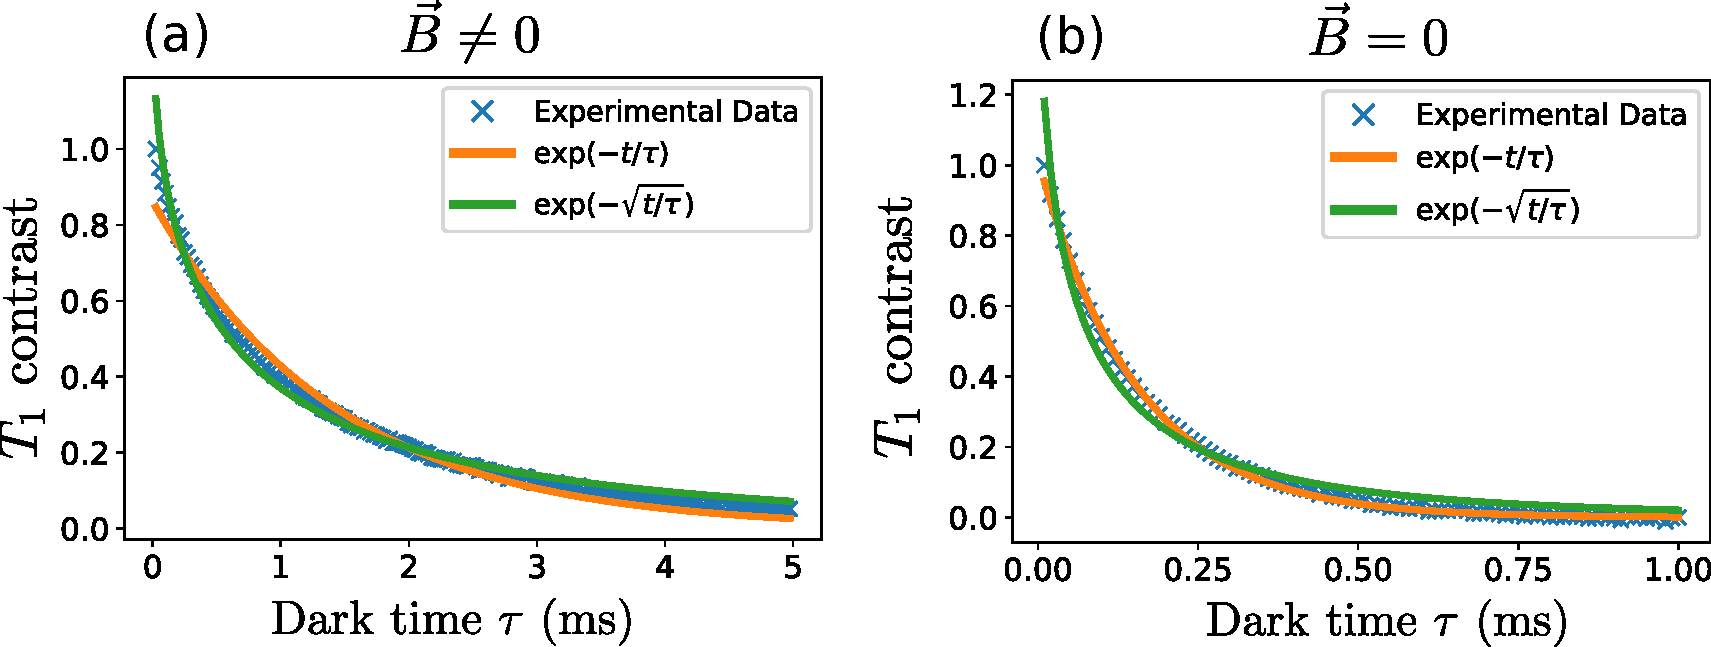
\includegraphics[width=\textwidth]{chapter 3/Figures/Anormal_T1}
\caption{$T_1$ measurements on sample ADM-15-4, fitted with pure exponential or stretched exponential. a) $T_1$ of a single isolated class when $\mathbf{B} \neq 0$. The optimal fit parameters are respectively $T_1^{\rm exp}=1.43\ \rm ms$ and $T_1^{\rm stretch}=0.56\ \rm ms$. b) $T_1$ of the four degenerate classes when $\mathbf{B}=0$. The optimal fit parameters are respectively $T_1^{\rm exp}=0.15\ \rm ms$ and $T_1^{\rm stretch}=0.05\ \rm ms$.}
\label{anormal T1}
\end{figure}

We mentioned previously that the discrepancy between the theoretical and experimental $T_1$  values were in contradiction with the current fluctuator model, although the difference could come in part from the $T_1$ fitting procedure. Another, more glaring problem is the fact that some $T_1$ profile are not stretched exponential.

Fig. \ref{anormal T1} shows $T_1$ measurement on sample ADM-15-4, either on a single isolated class ,where the dipole-dipole interactions are at their weakest, or on all four resonant classes at $\mathbf{B}=0$, where the interactions are at their strongest.

Although the spin lifetime still gets $\sim$ 10 times shorter in the $\mathbf{B}=0$ case, indicating that dipole-dipole interaction still plays an important role in the spin relaxation, this time the lifetime profile does not converge to a purely stretched exponential. In fact it seems to be the opposite: the lifetime profile is closer to a pure exponential for the shorter $T_1$ (especially for the very short times), and closer to a stretched exponential for the longer $T_1$, which is in complete contradiction with the fluctuator model and the previous observations in Fig. \ref{stretch_or_not_stretch} and \ref{various_fit_formulae}.

We should note that most sample studied follow the fluctuator model, in that the their lifetime profile gets closer to a stretched exponential when the dipole-dipole relaxation rate is increased. Sample ADM-15-4 seem to be an anomaly in this regard, since most of the samples from the same batch (including sample ADM-15-2 in Fig. \ref{stretch_or_not_stretch}) seem to follow the ``normal" behavior predicted by the fluctuator model. However, some other samples, including bulk HPHT samples and 150 $\mu$m Adamas micro-diamond also showed short (non stretched) exponential lifetimes.

It seems therefore that the current fluctuator model does not correctly describe the spin dynamics of every NV-dense samples. Looking at what was previously done for P-doped SI \citep{vugmeister1978spin} or for FRET \citep{yokota1967effects}, the fluctuator model could probably be improved by taking into account the finite lifetime of the fluctuators (i.e. the saturation of the NV-fluctuator CR), and the spin diffusion between NV centers (the fluctuator model only considers NV-fluctator interactions and not NV-NV interactions).

\subsection{Investigation of the fluctuators nature}
While the hypothesis of fluctuators being clusters of NV centers or NV-other spins is strengthened by the precedents in P-doped Si \citep{honig1960electron} or F centers in KCl \citep{warren1964spin}, there are still many unknowns on the exact nature of the fluctuators. There are at least two aspects that merit to be investigated.

The first one would be to study the fluctuator spectral profile on various samples showing NV-NV CR. In particular it would be interesting to know whether this profile is always Lorentzian, and what its linewidth is. In the sample studied on Fig. \ref{fluct linewidth}, we found a value for $\gamma_f$ surprisingly similar to the one found in \citep{choi2017depolarization}, even tough our sample only had $[\rm NV] \sim 3 ppm$ compared to the $[\rm NV] \sim 15 ppm$ sample used in \citep{choi2017depolarization} \footnote{Although the initial paper claimed a NV concentration $[\rm NV] \sim 45 ppm$, a more recent paper re-established the concentration at $\sim 15$ ppm \citep{zhou2020quantum}}. If $\gamma_f$ was found to be somewhat of a constant among all samples showing NV-NV CR, this would give us a lot of information on the potential nature of the fluctuators. Studying the temperature dependency of $\gamma_f$ could also give us information on whether the depolarization mechanism is due to tunneling or modulation of the $J-$coupling by the phonons.

The other aspect would be to identify potential defects that could form fluctuators when paired with NV centers. The main candidate for this would be substitutional nitrogen (P1 or P1$^+$ centers) since they are the most abundant electronic spin species in the diamond we use. The ideal way to confirm this hypothesis would be to compare the spin $T_1$ for  different samples with the same [NV] concentration, but different [P1] concentration. If indeed P1 centers play a role in the presence of fluctuators, we would expect a shorter NV $T_1$ time in the sample with high P1 concentration.



\chapter{NV-NV cross-relaxation at low magnetic field: application to magnetometry}

In the last chapter we have identified a dipole-dipole relaxation mechanism within dense NV centers ensemble, and we have studied its influence in non-zero magnetic field. In this chapter we will cover the low to zero magnetic field region and see how the depolarization at low magnetic field can be used for magnetometry.

This chapter is constructed as follows: We will first describe in sec. \ref{sec 4.1} the physics of NV centers under low or transverse magnetic field. In sec. \ref{sec causes zero field}
we will present the different zero field depolarization causes that we have identified as well as their theoretical impact on the NV relaxation rates according to the fluctuator model. In sec. \ref{sec 4.3} we will confront the predictions of the fluctuator model with experiments under low and transverse magnetic field. 

We will then focus on the low field depolarization magnetometry (LFDM) protocol which exploits the previously studied NV-NV CR at low magnetic field. We will start by giving a short overview of NV ensemble magnetometry in sec. \ref{sec 4.4} before characterizing the LFDM protocol in sec. \ref{sec LFDM} and comparing it to other magnetometry protocols in sec. \ref{sec 4.6}. Finally we will give some perspectives on how to improve LFDM and on potential applications.

The results presented in this chapter are based in large part on the article \citep{pellet2022spin}.

\section{NV spin Hamiltonian under low and transverse fields}
\label{sec 4.1}
We will start this chapter by studying the single NV physics under low and transverse magnetic field. On of the main difference with the previously studied regime is that the eigenstates of the Hamiltonian are no longer $\{ \ket{0}, \ket{+1}, \ket{-1} \}$, which will then in turn modify the dipole-dipole interaction between the NV centers.

We will first describe the spin Hamiltonian of the NV center under low magnetic field and determine the dominant factors in our samples, then do the same for transverse magnetic field, and finally investigate the modification of the ODMR lineshapes in those regimes.

\subsection{NV spin Hamiltonian in zero external magnetic field}
\label{sec. Hamltonian 0 B}
\begin{figure}[h]
\centering
\includegraphics[width=\textwidth]{chapter 4/Figures/ESR_simus}
\caption{Monte-Carlo simulations of inhomogeneous zero field ODMR for different noise sources. a) Magnetic noise: each of the $\mathbf{B}$ components is sampled over a Gaussian of deviation $\sigma=2\ \rm G$. b) Strain noise: each of the components of the strain tensor $\bar{\bar{\varepsilon}}$ is sampled over a Gaussian of deviation $\sigma=2\cdot 10^{-4}$. c) Electric noise: each of the $\mathbf{E}$ components is sampled over a Gaussian of deviation $\sigma=2\cdot 10^{5}\ \rm{V/cm}$. d) Experimental ODMR spectrum in zero external field taken on sample ADM-150-2}
\label{simus ESR}
\end{figure}

In the absence of a strong external magnetic field, the dominant terms of the NV spin Hamiltonian originate from local noises. These noises are: the random local magnetic fields caused by paramagnetic impurities, the local electric field caused by charged impurities, and the crystal strain \citep{doherty2012theory, udvarhelyi2018spin, mittiga2018imaging}. 

Due to the large zero field splitting $D=2870\ \rm MHz$ between the $\ket{0}$ and $\ket{\pm 1}$ states, we will consider the $\ket{0}$ state to always be an eigenstate of the spin Hamiltonian under zero external field. The problem is then reduced to the $\{ \ket{-1}, \ket{+1} \}$ subsystem.

The NV$^-$spin Hamiltonian in the $\{ \ket{-1}, \ket{+1} \}$ basis can be written as \citep{udvarhelyi2018spin}:
\begin{equation}
\mathcal{H}=\begin{pmatrix}
D-\gamma_e B_\parallel + f_\parallel(\mathbf{E}) + g_\parallel(\bar{\bar{\varepsilon}}) & f_\perp(\mathbf{E}) + g_\perp(\bar{\bar{\varepsilon}})\\
f^*_\perp(\mathbf{E}) + g^*_\perp(\bar{\bar{\varepsilon}})&D+\gamma_e B_\parallel + f_\parallel(\mathbf{E}) + g_\parallel(\bar{\bar{\varepsilon}})
\end{pmatrix},
\label{Hamiltonien pm1}
\end{equation}
where $B_\parallel$ is the component of the magnetic field along the NV axis, and $f_\parallel, f_\perp, g_\perp$, and $g_\parallel$ are functions of the electric field $\mathbf{E}$ and the strain tensor $\bar{\bar{\varepsilon}}$, whose expressions are:

\begin{align}
f_\parallel(\mathbf{E})&=d_\parallel E_z, \\
f_\perp(\mathbf{E})&=d_\perp ( E_x + i E_y), \\
g_\parallel(\bar{\bar{\varepsilon}})&= h_{41}(\varepsilon_{xx}+\varepsilon_{yy})+h_{43} \varepsilon_{zz}, \\
g_\perp(\bar{\bar{\varepsilon}}) &= \frac{1}{2} \left[ h_{16}(\varepsilon_{zx}+i \varepsilon_{zy}) + h_{15}\left(\frac{\varepsilon_{yy}-\varepsilon_{xx}}{2}+i\varepsilon_{xy}\right) \right],
\end{align}
where $d_\parallel=0.35 \ \rm{Hz\, cm/V}$ and $d_\perp=17\ \rm{Hz\, cm/V}$ have been measured experimentally \citep{van1990electric}, and $h_{43}=2300\ \rm{MHz}$, $h_{41}=-6420\ \rm{MHz}$, $h_{15}=5700\ \rm{MHz}$ and $h_{16}=19660\ \rm{MHz}$ were computed through DFT \citep{udvarhelyi2018spin} and show reasonable agreement with experiments \citep{barson2017nanomechanical}.

%Importantly, as pointed in \citep{mittiga2018imaging} we notice that both the electric field and the strain have a \textit{shifting} component ($f_\parallel$ and $g_\parallel$) which shifts equally both eigenstates of the Hamiltonian, and a \textit{splitting} component ($f_\perp$ and $g_\perp$) which splits in energy the two eigenstates. 
%
%The main difference between the electric field and the strain is in the numerical prefactors of these components: for the electric field, the splitting parameter $d_\perp$ is $\sim 50$ times higher than the shifting parameter $d_\parallel$, which will result on average to a strong energy split without much shifting. For the strain however, the splitting parameters $h_{15}$ and $h_{16}$ are only $\sim 3$ times higher than the shifting parameters $h_{43}$ and $h_{41}$. The shift in energy will therefore tend to blur the energy split when averaging over a large number of spins.

Fig. \ref{simus ESR}-a) b) and c) shows the result of Monte-Carlo simulations of the ODMR of an ensemble of NV centers for different noise sources. The simulation work as follow: one of the three possible noise source (magnetic field, electric field or strain) is sampled randomly while the two other are kept at zero. The eigenvalues of the spin Hamiltonian given in eq. \ref{Hamiltonien pm1} are then computed and the process is repeated $10^6$ times to create the histograms shown in Fig. \ref{simus ESR}.

Fig. \ref{simus ESR}-d) shows an experimental zero-field ODMR which is typical of the samples used in this manuscript. In particular we can notice a central splitting of the spectrum. This splitting is only present in the simulation when the dominant noise is the electric field. We then conclude that the dominant noise source in our sample (in the absence of external magnetic field) is the local electric field.

The authors of \citep{mittiga2018imaging} came to the same conclusion for the samples with dense NV ensemble that they studied by using a more sophisticated simulation model.

%We should note that another potential explanation for the splitting of the $\ket{\pm 1}$ states could be the presence of a residual magnetic field, not randomly distributed among all the spins but homogeneous on the whole sample. In particular, we do not shield for the earth magnetic field in our experiment. The splitting caused by the earth magnetic field however has a value $\gamma B_{\rm earth} \approx 1\ \rm MHz$, which is $\sim 4$ times weaker than the splitting we typically observe. 

Given that $d_\perp \approx 50 d_\parallel$, we can consider that the dominant electric field noise comes from the transverse electric field. We will then adopt the following simplified Hamiltonian for the zero external magnetic field regime:
\begin{equation}
\mathcal{H}=\begin{pmatrix}
D&0&d_\perp E_\perp^* \\
0&0&0 \\
d_\perp E_\perp &0&D
\end{pmatrix},
\end{equation}
whose eigenvectors are $\ket{0}$ and$\ket{\pm}$ of eigenvalues 0 and $D\pm d_\perp \abs{E_\perp}$, where $\ket{\pm}$ are defined as:
\begin{equation}
\ket{\pm}=\frac{\ket{+1}\pm e^{-i\phi_E}\ket{-1}}{\sqrt{2}},
\end{equation}
where $\tan(\phi_E)=E_y/E_x$.

\subsection{NV spin Hamiltonian under purely transverse magnetic field}
\label{sec B transverse}
%\begin{figure}[h]
%\centering
%\includegraphics[width=0.7\textwidth]{chapter 4/Figures/map_etats_propres}
%\caption{Closeness of the Hamiltonian most excited state $\ket{3}$ with either $\ket{+1}$ or $\ket{+}$ as a function of the external magnetic field amplitude and angle $\theta$ with respect to the NV axis.}
%\label{map champ transverse}
%\end{figure}

We now turn to the case of a magnetic field that is orthogonal to the NV axis, i.e. $\mathbf{B}=B_x \hat{e}_x + B_y \hat e_y$, and more specifically to the regime where $d_\perp E_\perp < \frac{(\gamma_e B_\perp)^2}{D} << D$. In practice, this generally corresponds to $20\ \rm G \lesssim B_\perp \lesssim 200\ \rm G$.

In this regime, the NV Hamiltonian eigenstates are similar to the case where it is dominated by the transverse electric field and can be written $\approx \ket{0}, \ket{-}, \ket{+}$\citep{qiu2021nuclear, qiu2022nanoscale}, of respective eigenvalues $\approx -\frac{(\gamma_e B_\perp)^2}{D},D,D+\frac{(\gamma_e B_\perp)^2}{D}$,  where:
\begin{equation}
\ket{\pm}=\frac{\ket{+1}\pm e^{-2i\phi_B}\ket{-1}}{\sqrt{2}},
\end{equation}
and $\tan(\phi_B)=B_y/B_x$.

For the case where $d_\perp E_\perp \sim \frac{(\gamma_e B_\perp)^2}{D}$ and $\phi_E \neq 2\phi_B$, the eigenstates of the Hamiltonian are still of the form $\ket{0},\ket{\pm}$ with a relative angle $\phi$ in between $\phi_E$ and $2\phi_B$.

In conclusion, whenever the spin Hamiltonian is dominated by the local electric field or by the transverse magnetic field, we can consider that the eigenstates of the spin Hamiltonian to be $\ket{0}, \ket{-}$ and $\ket{+}$, whereas when the Hamiltonian is dominated by the longitudinal magnetic field, its eigenstates are $\ket{0}, \ket{-1}$ and $\ket{+1}$.

\subsection{Hyperfine and inhomogeneous broadening}
\label{sec modif T2*}
\begin{figure}[h]
\centering
\includegraphics[width=\textwidth]{chapter 4/Figures/Comparaison_ESR_T2}
\caption{ODMR lineshapes for longitudinal, transverse and low magnetic fields on samples CVD-pink and Sumi-2. a) ODMR spectrum of a single class of NV centers for a longitudinal magnetic field ($B_\parallel \sim 100\ \rm G$). The microwave frequency is given with respect to the ODMR line central frequency. b) ODMR spectrum of a single class for a purely transverse magnetic field ($B_\perp \sim 100\ \rm G$). c) ODMR of all 4 classes for 0 external magnetic field. d) Table reporting the full width at half maximum of each ODMR line.}
\label{ESR for T2*}
\end{figure}

A consequence of the change in the Hamiltonian eigenstates from the $\{ \ket{0}, \ket{\pm 1} \}$ to the $\{ \ket{0}, \ket{\pm} \}$ basis is that the Hamiltonian eigenvalues are sensitive to different part of the environment. The energy of the $\ket{\pm 1}$ states depends linearly on the longitudinal magnetic field, and quadratically on the transverse electric and magnetic fields. On the contrary, the $\ket{\pm}$ states depend linearly on the transverse electric field, and quadratically on the longitudinal and transverse magnetic field \footnote{The transverse magnetic field is always of second order for weak magnetic field because $D\gg \gamma B_\perp$.}. 

The shape of the ODMR lines (i.e. the spectral response of the spins) is therefore dominated by the magnetic noise and the hyper-fine coupling in the $\{ \ket{0}, \ket{\pm 1} \}$ basis, and by the electric noise in the $\{ \ket{0}, \ket{\pm} \}$ basis, as we established in the previous part. Further details on the low magnetic field regime are available in \citep{jamonneau2016competition} and on the purely transverse magnetic field regime in \citep{qiu2021nuclear, qiu2022nanoscale}.

Fig. \ref{ESR for T2*} shows ODMR profile on two samples, CVD-pink which shows weak dipole-induced depolarization and Sumi-2 which shows strong dipole-induced depolarization, in three distinct regime: for a purely longitudinal magnetic field, for a purely transverse magnetic field, and without magnetic field. The linewidths of the spin transition \footnote{We consider here the full linewidth of the electronic levels, i.e. including all three hyper fine levels} for both samples are reported in the Table \ref{ESR for T2*}-d). In both cases, the linewidths are smaller in the $B=0$ and $B \perp NV$ cases than in the $B \parallel NV$ case, mainly due to the modification of the hyper-fine coupling. The linewidth modification reaches up to $\sim 50\ \%$ for the CVD sample and $\sim 20\ \%$ for the HPHT one.

We are particularly interested in the spin transition linewidth since it directly impacts the dipole-dipole relaxation rate (as seen in sec. \ref{sec computation eta}): the smaller the linewidth, the higher the dipole-dipole relaxation rate is.

\bigskip

To summarize this section, we have seen that (for the samples used in this chapter) the NV center spin Hamiltonian is dominated by transverse electric field at low external magnetic field, which causes a change of the Hamiltonian eigenstates from $\{ \ket{0}, \ket{\pm 1} \}$ to $\{ \ket{0}, \ket{\pm} \}$. 

We have also seen that the spin Hamiltonian has the same eigenstates for purely transverse magnetic field than it does for low magnetic field. 

Finally we have seen that this change of eigenstates occasions a modification of the spectral profile and linewidth of the spins.

\section{Theory of the low field depolarization}
\label{sec causes zero field}
\begin{figure}[h]
\centering
\includegraphics[width=\textwidth]{chapter 4/Figures/Shema_summary_theory_2}
\caption{Summary of the different depolarization effects in low magnetic field and their predicted depolarization rate. The ODMR spectra were taken on sample ADM-150-1}
\label{summary_theory}
\end{figure}

We will focus on this section on the mechanisms responsible for the depolarization of dense NV ensemble at low magnetic fields. We have identified four such mechanisms that lead to an increase in the resonant dipole-dipole coupling between NV and fluctuators, which in turn results in an increased spin depolarization rate.

Fig. \ref{summary_theory} summarizes these four mechanisms along with the theoretical increase in the depolarization rate caused by each of them. We will detail below the physical origin of these four mechanisms and the calculations that lead to the values presented in Fig. \ref{summary_theory}.

We should note that the values indicated in Fig. \ref{summary_theory} for the double flips and the $T_2^*$ contributions depend on experimental parameters, while the ones for the 4-classes degeneracy and the eigenbasis change are purely based on theory.

\subsection{Four classes degeneracy}

The first and main contribution to the low field depolarization is the degeneracy between the four classes as the magnetic field decreases. Following the arguments presented in the last chapter, the degeneracy between the four classes of NV centers causes in theory an increase in the relaxation rate by a factor $\sim 43$. This contribution is not specific to the zero field region, as we can observe the same resonance condition when $\mathbf{B} \parallel [100]$.


\subsection{Eigenstates modification}

The modification of the Hamiltonian eigenstates discussed in sec. \ref{sec. Hamltonian 0 B} from the eigenbasis $\{ \ket{0}, \ket{+1},\ket{-1} \}$ when $B\neq 0$ to the eigenbasis $\{ \ket{0}, \ket{+},\ket{-} \}$ when $B\sim 0$ changes the dipole-dipole interaction between the two spins. 

A consequence of this change is the absence of diagonal terms  in the dipole-dipole Hamiltonian written in the $\{ \ket{0}, \ket{+},\ket{-} \} \times \{ \ket{0}, \ket{+},\ket{-} \}$ basis, which explains why the NV centers states are protected from magnetic noises at low magnetic field \citep{jamonneau2016competition}. 

Another consequence is a slight modification of the flip-flop rates. Once averaged over all possible orientation and position, as detailed in appendix \ref{Appendix eta}, this modification of the flip-flop rates amount for an increase of $\Gamma_1$ by about $20\ \%$ in the $\{ \ket{0}, \ket{+},\ket{-} \}$ basis compared to the $\{ \ket{0}, \ket{+1},\ket{-1} \}$ basis.


\subsection{Double flips}

The double flip processes have been previously discussed in sec. \ref{sec flip-flop et double flip} and naturally arise from the dipole-dipole Hamiltonian. The ones that we consider here couple the states $\ket{0, \pm 1}$ and $\ket{\mp 1, 0}$ (in contrast with the flip-flop which couple the states $\ket{0, \pm 1}$ and $\ket{\pm 1, 0}$). These terms are generally not resonant because of the Zeeman splitting between the $\ket{+1}$ and $\ket{-1}$ states. 

In the low magnetic field regime however, we have to consider the new eigenstates $\ket{+}$ and $\ket{-}$ and the two-qubits states $\ket{0, \pm}$ and $\ket{\mp, 0}$. These terms are still not fully resonant because of the splitting between the $\ket{+}$ and $\ket{-}$ states caused by the local electric field, but they are close enough in energy that the double flip processes are not entirely suppressed.

The computation of the depolarization rate including the double flips is detailed in appendix \ref{Appendix eta}. To obtain a numerical value, we need to input the experimental values of the dipole-dipole interaction range \footnote{By interaction range we mean the value to be compared to the spectral detuning $\Delta \nu$ between the two groups. This is $2\gamma_f+\Gamma_{NV}+\Gamma_f$ in eq. (\ref{eq 1/T avec T2*})} which we measured to be $\Gamma=8.8\ \rm MHz$ in Fig. \ref{fluct linewidth}, as well as the average splitting $\Delta \nu$ between the $\ket{+}$ and $\ket{-}$ states. We typically measure $\Delta \nu \approx 8\ \rm MHz$ on type Ib HPHT samples.

For the value presented in Fig. \ref{simus ESR}, we inputted $\Gamma=\Delta \nu=8.8\ \rm MHz$.


\subsection{$T_2^*$ increase}

The last aspect we considered was the change in the ODMR lineshape discussed in sec. \ref{sec modif T2*} for weak magnetic field (we refer to the spectral linewidth as $T_2^*$ for conciseness).

To quantify the impact of the $T_2^*$ increase in the depolarization rate, we employ eq. (\ref{eq 1/T avec T2*}), where we use the values $2\gamma_f = 6.5\ \rm MHz$ estimated in the last chapter and we take for $\Gamma_f=\Gamma_{\rm NV}$ the values of half width at half maximum found in Fig. \ref{ESR for T2*}. We then find that the increase of $T_2^*$ in zero magnetic field occasions an increase of the decay rate by $\sim 9 \%$ for sample Sumi-2, and by $\sim 24 \%$ for sample CVD-pink. 

The value shown in Fig. \ref{summary_theory} corresponds to a $9 \%$ increase.

\bigskip

In conclusion, we predict that the 4-classes degeneracy is by far the dominant causes for low field depolarization ($\sim \Gamma_1 \times 40$), followed by the double flips ($\sim \Gamma_1 \times 2$). We will however see in sec \ref{sec LFDM} that the double flips, along with the change of eigenbasis and increase in $T_2^*$ are determinant factor in the sensitivity of the low field magnetometry protocol.

In the following section we will confront the theoretical results with experimental ones.

\section{Experimental investigation of the low field depolarization}
\label{sec 4.3}
In this section we will try to experimentally discriminate the contribution of the four depolarization sources described in Fig. \ref{summary_theory} and confront the experimental values with the theoretical ones. 

We will first determine the contribution of the 4-classes degeneracy by comparing [100] aligned and non-[100] aligned magnetic field in the weak magnetic field regime, before studying the influence of the double-flips thanks to purely transverse magnetic fields.

On top of the four previously discussed relaxation mechanisms, we have also considered two additional causes for the observation of low-field depolarization: the misalignment of the magnetic field (when $\mathbf{B}\parallel [100]$) and the influence of the laser polarization. Following further experiments detailed in appendix \ref{Appendix autres causes}, we have determined that these two effects were negligible compared to the four ones we identified before.

\subsection{NV-NV CR in the low magnetic field regime}


In this part, we will try to isolate the contribution of the 4-classes degeneracy from the three other ones by using the fact that all four classes can be at resonance for two distinct scenario:
\begin{itemize}
\item When $\mathbf{B}=0$.
\item When $\mathbf{B}\parallel [100]$ (cf. Fig. \ref{ODMR_geometries}).
\end{itemize}

\subsubsection{Magnetic scan in a random direction}

\begin{figure}[h]
\centering
\includegraphics[width=0.9\textwidth]{chapter 4/Figures/scan_1x1x1x1}
\caption{Low field depolarization on sample ADM-150-1 for $\mathbf{B}$ in an arbitrary direction. a) ODMR spectrum for B=0. b) ODMR spectrum for B=60 G. c) PL contrast as a function of the external magnetic field. d) $1/T_1^{\rm dd}$ as a function of the external magnetic field. A $T_1$ measurement was recorded for each magnetic field value and fitted accorded to the protocol described in Fig. \ref{various_fit_formulae} with $T_1^{\rm ph}=5\ \rm ms$}
\label{scan 1x1x1x1}
\end{figure}

First we will run a control experiment by scanning the magnetic field in a non [100] direction. Fig. \ref{scan 1x1x1x1}-a) and b) shows ODMR spectrum at the starting point ($|\mathbf{B}|=0$) and end point ($|\mathbf{B}|\approx 60\ \rm G$) of the magnetic field scan. The magnetic field orientation was chosen in order to maximize the splitting of the four classes.

Fig. \ref{scan 1x1x1x1}-c) and d) show the evolution of the NV PL and stretched lifetime $T_1^{\rm dd}$, defined in the last chapter, as a function of the magnetic field. We can observe a decrease of $T_1^{\rm dd}$ by a factor of $\sim 10$ in zero magnetic field compared to non-zero magnetic field, with a half-width at half maximum of $\sim 10\ \rm G$. Correspondingly, we can observe a drop in PL by $\sim 4\%$ in zero magnetic field \footnote{We can also note the decrease in PL for $|\mathbf{B}|> 30\ \rm G$ is not corroborated by an increase of $1/T_1^{\rm dd}$. This is because this drop of PL is associated with transverse magnetic field state mixing, and not with spin depolarization.}. 

We attribute the spin depolarization observed in Fig. \ref{scan 1x1x1x1}-d) to all four mechanisms described in the last part acting simultaneously. To determine the contribution of each mechanism individually, we will need to run dedicated experiments.

\subsubsection{Magnetic scan with $\mathbf{B} \parallel [100]$}

\begin{figure}[h]
\centering
\includegraphics[width=0.9\textwidth]{chapter 4/Figures/scan_100}
\caption{Same measurements as Fig. \ref{scan 1x1x1x1}, still on sample ADM-150-1, but with $\mathbf{B}$ along the [100] axis.}
\label{scan 100}
\end{figure}

This second experiment is similar to the last one except that the magnetic field was scanned in the [100] direction. Fig. \ref{scan 100}-a) and b) again show ODMR at the starting and ending point of the magnetic scan, while Fig. \ref{scan 100}-c) and d) show the PL and $1/T_1^{\rm dd}$ recorded during the scan.

The main difference with the previous experiment is that in this case, the degeneracy between the four classes is never lifted. We therefore attribute the increase in $1/T_1^{\rm dd}$ at low magnetic field to the three other identified mechanisms. The increase in the depolarization rate in zero field ($\sim 20\ \%$) as well as the decrease inPL ($\sim 0.5 \%$) are still present, but significantly smaller than in the previous case. We can note however that the half-width at half maximum of the zero field depolarization ($\sim 2\ \rm G$) is also smaller in this case.

We can also note a drop in PL and a corresponding increase of $1/T_1^{\rm dd}$ for $B \sim 20\ \rm G$ which corresponds to the NV$-^{13}$C-NV cross-relaxation discussed in sec. \ref{sec NV-13c-NV}. We can not explain however why the depolarization rate appear to be smaller at $B \sim 10\ \rm G$ than it is for $B > 30\ \rm G$.

The fact that the increase of the depolarization rate at zero field is about $\sim 50$ times weaker in Fig. \ref{scan 100} than it was in Fig. \ref{scan 1x1x1x1} confirms that the leading cause of depolarization in zero field is the degeneracy between the four classes of NV centers. 

\subsection{NV-NV CR under purely transverse magnetic field}

Thank to the two previous experiments, we were able to discriminate the contribution of the 4-classes degeneracy from the three other mechanisms that are which are the eigenbasis change, the double-flips and the $T_2^* increase$. We now seek to discriminate the contribution of each of these three mechanisms.

We unfortunately were not able to discriminate the change of eigenbasis from the $T_2^* increase$, which would likely require a statistical study over different samples with different $T_2^*$ values. We were however able to discriminate the double flip contribution from the two other ones by scanning the magnetic field in a direction orthogonal to one NV class ($\mathbf{B} \perp [111]$).

\subsubsection{Principle of the experiment}
\begin{figure}[h]
\centering
\includegraphics[width=\textwidth]{chapter 4/Figures/transis_transverse_field}
\caption{Simulation of the eigenstates of the NV Hamiltonian for  a purely transverse magnetic field $B_\perp$. In addition to the transverse magnetic field, we consider a fixed transverse electric field of value $d_\perp E_\perp=4\ \rm MHz$. (a) Eigenvalues for the spin Hamiltonian as a function of $B_\perp$. The three states are labeled $\ket{1}$, $\ket{2}$ and $\ket{3}$. (b) Splitting between the $\ket{2}$ and $\ket{3}$ states (blue curve) and closeness factor $\abs{\bra{3}\ket{+}}^2$ between the $\ket{3}$ and $\ket{+}$ (red curve)}
\label{eigenstates transverse field}
\end{figure}

The idea behind the experiment is that the Hamiltonian eigenbasis is the same (or close to be the same) when $\mathbf{B}=0$ than it is when $\mathbf{B} \perp [111]$, as described in sec. \ref{sec B transverse}. For simplicity, we will assume here that both the magnetic field and the transverse electric field lies along the NV $x$ axis : $\mathbf{B}=B_x \hat{e}_x$ and $\mathbf{E}_\perp =E_x \hat{e}_x$

Fig. \ref{eigenstates transverse field} shows a simulation of the eigenstates and eigenenergies for a NV Hamiltonian subject to transverse electric field and magnetic field. We labeled the eigenstates of the Hamiltonian $\ket{1}$, $\ket{2}$ and $\ket{3}$ in ascending order of energy.

Fig. \ref{eigenstates transverse field}-b) shows both the splitting $\Delta \nu$ between the $\ket{2}$ and $\ket{3}$ states, and how close the $\ket{3}$ state is to the $\ket{+}=\frac{\ket{+1}+\ket{-1}}{\sqrt{2}}$ state via the factor $\abs{\bra{3}\ket{+}}^2$. We should note that with the assumption that $B_\perp \parallel E_\perp$, the $\ket{2}$ state is strictly equal to the $\ket{-}$ state regardless of the magnetic field amplitude.

These two metrics, $\Delta \nu$ and $\abs{\bra{3}\ket{+}}^2$ are the relevant parameters of the experiment: the goal is to increase $\Delta \nu$ to the point where the double flips are completely suppressed, while $\abs{\bra{3}\ket{+}}^2$ remains close to 1 in order to preserve the eigenbasis and $T_2^*$ contribution. Based on the plots in Fig.\ref{eigenstates transverse field}-b), the region with $B_\perp \in$ [100 G,200 G] seems to satisfy both these criteria: $\Delta \nu\,(100\ \rm G) \approx 30\ \rm MHz \gg \gamma_f$\footnote{Technically, $\Delta \nu$ is to be compared with the dipole-dipole interaction width $2\gamma_f+\Gamma_{NV}+\Gamma_f$ which we measured to be $\Gamma=8.8\ \rm MHz$ in Fig. \ref{fluct linewidth}.} and $\abs{\bra{3}\ket{+}}^2\, (200\ \rm G) \approx 0.96$.

Ideally, we would have used an electric field instead of a transverse magnetic field to split the 4 classes energetically, but such an electric field would need to be $> 10^6\ \rm{V/cm}$ which is several order of magnitudes greater than the breakdown voltage of air and out of our experimental reach.

\subsubsection{Results}

\begin{figure}[h!]
\centering
\includegraphics[width=.8\textwidth]{chapter 4/Figures/scan_T1_perp}
\caption{Experimental data for the depolarization under purely transverse magnetic field on sample ADM-150-2. a) ODMR spectrum for $|\mathbf{B}|=20\ \rm G$. The transitions of the class orthogonal to the magnetic field are labeled $\nu_+$ and $\nu_-$. b) Dependency of $\nu_+$ and $\nu_-$ with the magnetic field, as measured through ODMR. c) Measurement of $T_1^{\rm dd}$ as a function of the transverse magnetic field. The corresponding energy splittings $\Delta \nu=\nu_+-\nu_-$ are written on top. We divided the plot between the A region where $1/T_1^{\rm dd}$ decreases, and the B region where it reaches a plateau with a value $1/T_1^{\rm dd}=185 \pm 5\ \rm s^{-1}$. We also indicate in green the value found for a purely longitudinal magnetic field $1/T_1^{\rm dd}=126 \pm 10\ \rm s^{-1}$}
\label{champ tranverse exp}
\end{figure}

Fig. \ref{champ tranverse exp}-a) shows an ODMR spectrum for $B=20\ \rm G$ with the two central lines corresponding to the $\ket{0} \to \ket{+}$ and $\ket{0} \to \ket{-}$ transitions of the class orthogonal to the magnetic field. We decided to start the scan of the magnetic field at $20\ \rm G$ because the class orthogonal to $\mathbf{B}$ was far enough ($> 20 MHz\ \rm MHz$) from the three other ones that flip-flop between them could be neglected\footnote{The small plateau at the beginning of the $1/T_1^{\rm dd}$ curve in Fig. \ref{champ tranverse exp}-c) confirms that flip-flop between the class orthogonal to $\mathbf{B}$ and the three other classes are indeed negligible compared to the other depolarization factors.}

Fig. \ref{champ tranverse exp}-b) shows the evolution of the $\nu_+$ and $\nu_-$ transition frequencies as a function of the magnetic field, measured via ODMR. The difference in frequency $\Delta \nu = \nu_+ - \nu_-$ is at first determined by the transverse electric field ($\sim 9\ \rm MHz$) and then grows qudratically with the transverse magnetic field up to a value of $\sim 50\ \rm MHz$.

Fig. \ref{champ tranverse exp}-c) shows the evolution of $1/T_1^{\rm dd}$ on a single class as a purely transverse magnetic field is scanned from 20 to 130 G. It also includes the $1/T_1^{\rm dd}$ value found for a purely longitudinal magnetic field which we will consider as a baseline, since the eigenbasis in this case is $\ket{\pm 1}$ and not $\ket{\pm}$. We have divided the graph in two regions labeled A and B:

In region A, $1/T_1^{\rm dd}$ decreases with the magnetic field. The difference in the depolarizing rate between the $\mathbf{B} \perp [111]$ case and the $\mathbf{B} \parallel [111]$ case comes from the double flips, the eigenbasis change and the $T_2^*$ increase. We measure an increase by a factor $\sim 3$ for B=20 G compared to the baseline.

In region B, $1/T_1^{\rm dd}$ reaches a plateau with a value of $\sim 180\ \rm s^{-1}$. We attribute this plateau to the fact that the double flips are completely quenched, which is coherent with the fact that $\Delta \nu \geq 30\ \rm MHz$. The remaining difference between the $\mathbf{B} \perp [111]$ and $\mathbf{B} \parallel [111]$ cases therefore comes from the eigenbasis change and the $T_2^*$ increase. This increase amount for $\sim$ 50\% of the relaxation rate baseline.

We should note that the theoretical increase from the double flips and the change of eigenbasis\footnote{The $T_2^*$ increase should still amount for $\sim 10\%$.} are not the values shown in Fig. \ref{summary_theory}: those were computed for a 4-class resonance, while we are looking here at a single class. The theoretical increase of the depolarization rate for a single class are detailed in Appendix \ref{Appendix eta}. They are:
\begin{itemize}
\item $\Gamma_1^{\ket{\pm}}=4 \Gamma_0$ when taking into account the change of eigenbasis.
\item $\Gamma_1^{dd}=1.6\Gamma_1^{\ket{\pm}}=6.5\Gamma_0$ when taking into account the double flips.
\end{itemize}
We have labeled here $\Gamma_0$ the relaxation rate coming from the flip-flop inside of a single class in the $\ket{\pm 1}$ basis (same definition as in table \ref{T1 champ mag} (table des valeurs chap 3). Experimentally, $\Gamma_0$ corresponds to the baseline shown in Fig. \ref{champ tranverse exp}-c).

Although we find again that the fluctuator model overestimates the actual relaxation rates, these experimental observations still confirm the qualitative predictions of the model. In particular, they confirm that the double-flips are the second leading cause of zero-field depolarization after the 4-classes degeneracy.

\subsection{Conclusion of the experimental observation}

\begin{figure}[h!]
\centering
\includegraphics[width=\textwidth]{chapter 4/Figures/Shema_summary_exp}
\caption{Summary of the different experimental investigation. A baseline value is indicated with the pink shaded region in all experimental plots. The left box indicates the relaxation mechanisms added compared to the baseline for the minimum value of B, and the right box those for the maximum value of B. (a) corresponds to Fig. \ref{scan 1x1x1x1}-d) where the baseline was measured to be $220\pm 20$ s$^{-1}$, (b) corresponds to Fig. \ref{scan 100}-d) with the same baseline, and (c) corresponds to Fig. \ref{champ tranverse exp}-c).}
\label{summary_exp}
\end{figure}

Fig. \ref{summary_exp} summarizes the experimental results of this section. We explicitly indicates which of the four depolarization mechanisms are responsible for the observed depolarization rate at the beginning and at the end of each curve.

The experiments confirm the overall predictions of the previous section: the dominant cause of depolarization in zero magnetic field is the degeneracy of the 4 NV classes, followed by the double-flips and then by the eigenbasis change and $T_2^*$ increase.

We will now cover the low-field magnetometry protocol, after a quick overview of the field of NV magnetometry, and see the role that the different depolarization mechanisms play in it.


\section{Introduction to ensemble NV magnetometry}
\label{sec 4.4}

There are two classes of NV magnetometer: single NV or ensemble. Single NVs offer a spatial resolution limited only by how far the magnetic source can be from the NV center (down to $\sim 10\ \rm nm$), but at the cost of a relatively low sensitivity (typically $\sim \mu \rm{T} / \sqrt{\rm Hz}$ \citep{pelliccione2016scanned}).

Ensemble NV centers center on the other hand offer sensitivities as low as $1\ \rm pT / \sqrt{\rm Hz}$ \citep{wolf2015subpicotesla}, at the cost of working with samples of sizes up to several mm.

We will only focus in this section on NV ensemble magnetometry since we want to give elements of comparisons with our technique based on NV-NV CR. We will not try to give a complete overview of this field, but only of the elements close to the technique we present. For a general overview on NV magnetometry, we recommend the excellent reviews  \citep{rondin2014magnetometry, degen2017quantum, barry2020sensitivity}.

\subsection{AC and DC magnetometry}
The most sensitive NV magnetometry protocols use the free precession of the spins to map a small change in the Zeeman energy into the phase of the spins, which is then converted into spin population. These protocols are generally separated between DC-broadband and AC-narrow band.

For DC-broadband magnetometry, the general technique consists of a Ramsey interferometry experiment, presented in chapter 1, the sensitivity of which is limited by the spin inhomogeneous coherence time $T_2^*$ (which can reach up to $\ \rm{\mu s}$ for NV ensembles). The bandwidth of the protocol is limited by the repetition rate of the experiment, generally up to $\sim 100\ \rm kHz$. Although less sensitive in theory, continuous-wave (CW) ODMR and pulsed ODMR are also often employed for DC magnetometry. The state of the art DC ensemble magnetometr operates with a sensitivity of $\sim 20\ \rm pT/ \sqrt{\rm Hz}$ \citep{barry2016optical, chatzidrosos2017miniature}.

For AC magnetometry, the basic protocol consists of a spin echo measurement, also presented in chapter 1, which extends the coherence time $T_2^*$ to $T_2 = 10 \sim 100 \rm{\mu s}$, and which can be extended even further to $\sim \rm ms$ times with dynamical decoupling \citep{pham2012enhanced}. Due to the longer ``free" precession time, a larger phase can be imprinted on the spin for a similar magnetic field. The AC magnetic field however has to be in phase with the rephasing pulses, which limits the AC sensing to a relatively narrow band. The state of the art in term of AC sensing is $\sim 1\ \rm pT/\sqrt{\rm Hz}$ \citep{wolf2015subpicotesla}.

Recently, \citep{xie2021hybrid} have achieved new records in both DC ($\sim 200\ \rm fT/\sqrt{\rm Hz}$) and AC ($\sim 10\ \rm fT/\sqrt{\rm Hz}$) NV magnetometry by using flux concentrators which are ferromagnets concentrating the magnetic field in a small volume, similarly to an electromagnet. The technology of flux concentrator could be applied to any NV magnetometry protocol. We will here only compare experimental results obtained without a flux concentrator.

\subsection{Low field magnetometry}
Magnetometry at low magnetic fields ($\gamma B < d_\perp E_\perp$) is challenging since in this regime the NV eigenstates and eigenenergies do not depend on the magnetic field to the first order. This complication is often lifted  by simply using a bias magnetic field.

Some systems however need to be kept under low to zero external magnetic fields, for example to study the J-coupling between spins \citep{sutter2012computational}, or the phase of skyrmions \citep{zazvorka2020skyrmion}. To study these systems with NV centers, new protocols for low field NV magnetometry are required.

The main technique for low field magnetometry consists in using circularly polarized microwaves, which can only excite the $\ket{0} \to \ket{-1}$ and $\ket{0} \to \ket{+1}$ transitions, even when these states are not the Hamiltonian's eigenstates \citep{mrozek2015circularly, zheng2019zero, lenz2021magnetic, vetter2022zero}. These states are linearly dependent on the magnetic field and can therefore be used to perform magnetometry. The best sensitivity achieved with this technique was $250\ \rm pT/\sqrt{\rm Hz}$ \citep{zheng2019zero}.

Another technique consists in using the $^{13}\rm{C}-$NV complex we discussed in sec. \ref{sec NV-13c-NV} which because of the magnetic field offset caused by the $^{13}\rm{C}$ nucleus are first order sensitive to the magnetic field even in zero external magnetic field \citep{wang2022zero}. With natural abundance $^{13}\rm{C}$ however, this means that only $\sim 3\%$ of the NV centers are used, and increasing the $^{13}\rm{C}$ concentration can lower the coherence of the NV centers. 

\subsection{Microwave-free DC magnetometry}
All the previously described magnetemetry protocols relied on the use of a controllable microwave field to coherently manipulate the NV spin state.

%There are other protocols which correlate the magnetic field to the spin $T_1$ time (relaxometry). These protocols can operate without microwave field and work for either DC or high frequency AC sensing.

%\subsubsection{microwave-less DC magnetometry}
The DC microwave-free protocols rely on sharp features in the PL for specific magnetic fields values. Fig. \ref{CR P1 exp} in chapter 2 show such PL features, in particular the ground state level anti-crossing (GSLAC, simply labeled LAC on the figure), the sharpest of these features.

The GSLAC occurs for a purely longitudinal magnetic field where $\gamma B_z = D$, which corresponds to $B=1024\ \rm G$. In these conditions, the normally bright $\ket{0}$ state and the dark $\ket{-1}$ state become resonant and any residual mixing between these two states (coming from the electric field, the strain or the residual transverse magnetic field) will cause a drop in the NV polarization, and in the PL \citep{broadway2016anticrossing}. 

A protocol based on the GSLAC line has been implemented, first only for longitudinal magnetic field measurements \citep{wickenbrock2016microwave} and then for 3D vector measurement \citep{zheng2020microwave} with a sensitivity $\sim 300\ \rm pT/\sqrt{\rm Hz}$.

Another DC microwave-less protocol was proposed based on NV-NV CR \citep{akhmedzhanov2017microwave, akhmedzhanov2019magnetometry}. This technique reconstructs the external magnetic field by scanning an other magnetic field, similar to Fig. \ref{equivalent NV-NV} in chapter 3, and by measuring the position of the NV-NV CR lines. The 3D external magnetic field can then be recovered by scanning the magnetic field in different directions. The author of this paper did not measure the sensitivity of this protocol, but they predict a shot noise limited sensitivity of $24.7\ \rm nT/\sqrt{\rm Hz}$.

%\subsubsection{microwave-less AC magnetometry}
%The AC microwave-less protocols rely on a direct excitation of the $\ket{0} \to \ket{-1}$ or $\ket{0} \to \ket{+1}$ transitions by the magnetic field probed. The detection bandwidth is adjusted with an external DC magnetic field to bring the NV transitions in resonance with the field probed, which has been implemented from $\sim 10\ \rm MHz$ to $27\ \rm GHz$ \citep{magaletti2022quantum}.
%
%Sensitivities as low as a few $\rm pT/\sqrt{\rm Hz}$ have been recorded near 2.87 GHz \citep{wang2022picotesla, alsid2022solid}, but both protocols are not microwave-free as they rely on a secondary controllable microwave field (either for an heterodyne detection or to add additional pulses).

\subsection{Orientation-free magnetometry}
All protocols described so far require precise knowledge of the Larmor frequency between the $\ket{0}$ and $\ket{\pm 1}$ states for a given magnetic field. This knowledge implies that the direction of each NV axis in the frame of the magnetic field is known, because of the strong anisotropy in the NV Hamiltonian. 

For a single crystal, these axes can always be calibrated through ODMR. However, for a polycrystalline diamond, diamond powder or even a single diamond with an erratic motion, the knowledge of these axes is not possible. New protocols need to be found if one wants to perform magnetometry with these materials.

To our knowledge, the only known orientation-free protocol for DC magnetometry is to use the change in PL caused by the transverse field, which is a property that depends only weakly on the field orientation, especially with an ensemble of NV centers with multiple axes. This protocol has a very low sensitivity but is still sometimes used in the absence of alternative \citep{rondin2012nanoscale, tetienne2012magnetic, maletinsky2012robust, chapman2013background, jones2020selective, zhu2022sunlight}.

Orientation-free magnetometry can also be performed for noise sensing, provided that that the noise is sufficiently broadband to directly excite the NV transitions regardless of their Larmor frequencies. The noise can be probed either by measuring the spin $T_1$ time \citep{kolkowitz2015probing, andersen2019electron} (which does not require a knowledge of the Larmor frequency), or via the PL \citep{finco2021imaging}.

\section{Low field depolarization magnetometry}
\label{sec LFDM}
We will now present and characterize the low field depolarization magnetometry (LFDM) protocol which rely on the depolarization of dense NV ensemble at low magnetic field. This protocol works for DC or slowly varying ($\lesssim 10\ \rm kHz$) magnetic field, is microwave-free, orientation-free, and operates at low magnetic field, although a small additional AC field is required to improve performances.

We will first describe its operation and characterize it before comparing it to the previously mentioned NV magnetometry protocols.

\subsection{Principle of the experiment}

\begin{figure}[h!]
\centering
\includegraphics[width=\textwidth]{chapter 4/Figures/setup_magneto}
\caption{Principle of the LFDM protocol a) Experimental setup. The confocal microscopy setup is similar to the one described in sec \ref{Sec setup cahp 1}, the lock-in amplifier (LIA) is used here to add a modulation on the magnetic field, instead of the microwave. Both the PL and the LIA signal are monitored. b) example of LIA signal on sample ADM-15-4 when scanning the magnetic field $B_0$ between -150 and 150 G. c) PL signal corresponding to the LIA signal}
\label{setup magneto}
\end{figure}

Fig. \ref{setup magneto} shows the principle of the LFDM protocol. The experimental setup is similar to the one presented in chapter 1 without any microwave field. The magnetic field generated by the electro-magnet contains both a DC or slowly variable component $B_0$ and an oscillating component $\tilde{B}_{\rm AC}$ used for the modulation. We typically use a modulation frequency $f_{\rm mod} \approx 1\ \rm kHz$, the same value we use for ODMR measurements. The main voltage $V_0$ responsible for the DC field and the oscillating voltage $\tilde{V}_{\rm AC}$ responsible for the AC field are summed via a homemade bias tee.

Fig. \ref{setup magneto}-b) and c) show the PL measured on the photodiode and on the lock-in respectively, when the DC magnetic field is slowly varied ($f_{\rm scan}<1\ \rm Hz$) from -150 to +150 G. For this configuration, the magnetic field was randomly oriented with respect to the NV axes and did not match any particular crystalline axis.

Both AC (up to $\sim$ 10 kHz) and DC-magnetometry are possible with this setup. To improve the sensitivity however, an AC field needs to be added for the DC sensing, and inversely a DC field needs to be added for the AC sensing. Both of these added fields are typically of a few G for optimal performances, which limits the ultra-low field applications.

\begin{figure}[h!]
\centering
\includegraphics[width=0.9\textwidth]{chapter 4/Figures/AC_and_DC_sensing}
\caption{DC and AC LFDM sensing protocols on sample ADM-15-5. The magnetic field is scanned in an arbitrary direction. a) DC sensing: $B_0$ is scanned between $-$80 and +80 G while an AC field of amplitude 10 G is used for the lock-in detection. b) AC sensing: $B_0$ scans are performed for 5 different $|\tilde B_{\rm AC}|$ values between 2 and 10 G. The best AC sensitivity is achieved for $B_0\approx 5\ \rm G$.}
\label{AC and DC sensing}
\end{figure}

Fig. \ref{AC and DC sensing} shows how the AC and DC sensing work for LFDM: for DC sensing the LIA signal around $B_0=0$ provide a sharp linear slope to convert the LIA voltage into a magnetic field. For AC sensing, the LIA signal is directly proportional to the amplitude of the field. The optimal AC field amplitude for DC sensing has to match the width of the PL dip $|\tilde{B}_{\rm AC}| = \sigma \approx 10\ \rm G$ in order to maximize the slope of the lock-in signal around $B_0=0$. the optimal DC field to use for AC sensing is $B_0= \sigma/2$ corresponding to the region where the lock-in signal is most sensitive to AC field. 

\subsection{Sensitivity of the LFDM protocol}
\begin{figure}[h!]
\centering
\includegraphics[width=\textwidth]{chapter 4/Figures/sensi_alternee}
\caption{Sensitivity measurement of the LFDM on sample ADM-15-4. a) Temporal trace of the LIA signal when applying an alternating external magnetic field of amplitude 35 $\mu$T and frequency $f=1\ \rm Hz$. b) Histogram of the DC measurement over 50 s. The data is fitted with Gaussians of width $1.6\ \rm{\mu T}$.}
\label{sensei alternee}
\end{figure}

We will now look at the performances of the LFDM protocol before comparing it to the other magnetometry protocols. The characterization was only done for DC sensing. The samples used for the characterization were 15 $\mu$m micro-diamond bought as is from Adamas nanodiamond (see sample details in appendix \ref{Appendix samples}).

We characterize the DC sensitivity by looking at the noise floor on the LIA signal when sitting on the steepest sloped ($B_0\approx 0$). The following parameters were used: $|\tilde{B}_{\rm AC}|\approx 10\ \rm G$ and $f_{mod} \approx 1\ \rm kHz$, the laser power was $\approx 1\ \rm mW$ and the collected PL power $\approx 1\ \rm{\mu W}$. The lock-in low-pass filter time constant was set to $\tau=3\ \rm ms$.

Fig. \ref{sensei alternee} shows the sensitivity measurement protocol. First, the applied magnetic field is calibrated with ODMR spectra, then an alternating DC field of known amplitude (here $\Delta B_0=35\ \rm{\mu T}$) is applied on the sample. Fig. \ref{sensei alternee}-a) shows the temporal trace of the LIA signal in response to this alternating DC field. Knowing the amplitude of the alternating field, we can then convert the voltage signal into a magnetic field amplitude, with in this case a ratio $45 \pm 3\ \rm{\mu T /V}$.

Fig. \ref{sensei alternee}-b) shows an histogram of the measured magnetic field amplitude for both the high and low value of the applied magnetic field. The total acquisition time was 50 s with the external field being alternated every second. The histograms are nicely fitted with Gaussian profiles of width $\sigma=1.5\pm 0.1\ \rm{\mu T}$ which allows us to estimate the DC sensitivity of the protocol:
\begin{equation}
\eta = \frac{\sigma}{\sqrt{2 \tau}}= 116 \pm 10\ \rm{nT} / \sqrt{\rm Hz},
\end{equation}

where $\tau=3\ \rm ms$ is the LIA low-pass filter time constant. 

We estimate that the sensitivity is mostly shot-noise limited because the same LIA voltage noise ($\sqrt{\langle \delta V^2 \rangle} \approx 35\ \rm mV$) was observed on a magnetic insensitive region (for $B_0 \approx 100\ \rm G$), and is far above the electrical noise measured when no optical signal is sent to the photodiode ($\sqrt{\langle \delta V^2 \rangle} < 1\ \rm mV$). The remaining noise could also come from laser intensity fluctuations.

\subsection{Angular dependence of the sensitivity}
\label{sec angular sensi}
\begin{figure}[h!]
\centering
\includegraphics[width=\textwidth]{chapter 4/Figures/sensi_angulaire}
\caption{Angular dependence of the sensitivity. a) LIA signal for $B_0$ scanned between $-$150 and +150 G along the [100] axis, or along a direction 20$^\circ$ off the [100] axis. b) Zoom-in of the LIA signal on the zero-field slopes. c) Measured sensitivity as a function of the magnetic field angle with the [100] axis.}
\label{angular sensi}
\end{figure}

We will now study the dependence of the sensitivity with respect to the magnetic field angle. In particular, we will compare the sensitivity for two scenarios: the case $\mathbf{B}\parallel [100]$and the four classes remains degenerate when $\mathbf{B}$ increases, and the case $\mathbf{B}\nparallel [100]$ where there is a lift of degeneracy between the four classes. We previously saw in Fig. \ref{scan 1x1x1x1} and \ref{scan 100} that the PL and $T_1$ contrast was much smaller when $\mathbf{B}\parallel [100]$, but we now focus on the sensitivity which is related to the slope of the PL change, and not directly to the contrast.

Fig. \ref{angular sensi}-a) and b) show the LIA signal when the DC field $B_0$ is scanned from $-150$ G to +150 G on the same sample ADM-15-4, but for two different angles of $B_0$. For the blue curve the field was scanned along the [100] axis, while for the orange curve it was scanned with an angle of $\sim 20\ ^\circ$ compared to the [100] axis. We can see that the maximum amplitude of the lock-in signal (relevant for AC sensing) is of the same order of magnitude for both case, and the slope around $B_0$ (relevant for DC sensing) is almost identical. Fig. \ref{angular sensi}-c) shows the sensitivity, measured with the protocol described in Fig. \ref{sensei alternee}, with respect to the angle between the magnetic field and the [100] axis. We can notice that the sensitivity depends only weakly on the magnetic field angle. 

The fact that the sensitivity is similar when $\mathbf{B}\parallel [100]$ or $\mathbf{B}\nparallel [100]$ means that the degeneracy between the four classes plays a lower role in the sensitivity than the three other mechanisms detailed in sec. \ref{sec causes zero field}. We cannot measure the individual impact of each of these three mechanisms, but based on the experimental results shown in Fig. \ref{champ tranverse exp}, we can assume that the double-flips are the dominant factor in the LFDM sensitivity.

It should be noted that this low angular dependence was particularly marked on sample ADM-15-4. Other samples, including from the same batch, showed a higher angular dependence with typically a sensitivity $2 \sim 3$ times worse for $B\parallel [100]$ than for the other directions.

\subsection{Temporal stability}
\begin{figure}[h!]
\centering
\includegraphics[width=\textwidth]{chapter 4/Figures/Temporal_just_0B}
\caption{Temporal stability of DC-LFDM as measured on sample ADM-15-5. a) Temporal trace of the LIA signal for $B_0 \approx 0$. The Lock-in signal was converted to a measured magnetic field with the previously described protocol. b) Estimated signal to noise ratio for a signal of 100 nT as a function of the total acquisition time $T$. The noise value is computed by averaging the variance of the temporal trace over each time duration $T$. A curve $y=0.5\, T^{1/2}$ is added for comparison}
\label{temporal 0B}
\end{figure}

An important aspect of sensors is their stability in time. The sensitivity being expressed in $\rm{nT} / \sqrt{\rm Hz}$ suggests that the signal to noise ratio (SNR) given by repeating the measurement increases as $\sqrt{T}$ where $T$ is the total acquisition time. This is true for an ideal system, but in practice drifts and low frequency noise mean that the actual SNR for long acquisition time will be worse than the SNR at short time scaled by a factor $\sqrt{T}$.

One of the main source of drift for NV magnetometry based on spin resonance is the crystal lattice temperature change: the $D$ factor in the NV Hamiltonian (eq. (\ref{eq. spin elec})) is sensitive to the lattice temperature because of the thermal dilatation of the crystal, which is the basis for NV thermometry \citep{kucsko2013nanometre}. This means that thermal fluctuations will impact the Larmor frequency of the spins and may cause a detuning with the initial measured frequency for long acquisition times. The LFDM protocol however does not rely on a specific resonance frequency, but rather on a co-resonnance condition between neighboring spins, which does not depend directly on the crystal temperature.

Fig. \ref{temporal 0B} shows the temporal stability of the LFDM protocol over an acquisition time of 100 s. Fig. \ref{temporal 0B}-a) shows a temporal trace of the LIA signal where we have converted the signal into a measured magnetic field. Fig. \ref{temporal 0B}-b) shows the estimated SNR for a signal of 100 nT as a function of the total acquisition time and was computed from the temporal trace.

We can see that the SNR does not deviate from the $\sqrt{T}$ scaling for times up to 50 s, and could probably be extended for longer times. The non-linearity for shorter times comes from the LIA low-pass filter.

\section{Comparison between LFDM and other magnetometry protocol}
\label{sec 4.6}
Now that we have characterized the LFDM protocol, we can compare its performances with the previously mentioned magnetometry protocols. The best sensitivity achieved with the LFDM ($\sim 100 \rm{nT} / \sqrt{\rm Hz}$) is about $10^5$ times worse than the best NV ensemble sensitivity. This discrepancy however come in large part to the smaller sensor volume used in the characterization, and to a relatively low PL collection efficiency compared to the other experiments.

\subsection{Comparison with microwave based protocols}

\begin{table}[htbp]
\centering
\caption{Comparison of the volume-normalized sensitivity of the best AC and DC protocols with LFDM}
 \label{table sensi volumiques}
\begin{tabular}{c|ccc}
\toprule
{} & Zhou et al. \citep{zhou2020quantum} (AC) & Barry et al.\citep{barry2016optical} (DC) & LFDM (DC) \\
\midrule
$\eta\ (\rm{nT} / \sqrt{\rm Hz})$ & 92&0.015& 116 \\
$V\ (\mu \rm{m}^3)$ &$8.1 \cdot 10^{-3}$ &$5.2 \cdot 10^{6}$& $3.3 \cdot 10^{3}$ \\
$\eta_v\ (\rm{nT}\mu \rm{m}^{3/2} \rm{Hz}^{-1/2})$ &8.3&34&6700 \\
\bottomrule
\end{tabular}
\end{table}

A better metric than the sensitivity to compare different protocols is the volume-normalized sensitivity defined in \citep{zhou2020quantum} as $\eta_v=\eta\cdot \sqrt{V}$ where $\eta$ is the sensitivity and $V$ the effective volume of the sensor. This scaling assumes that each NV center in an ensemble is an independent magnetic field probe, and as the total number of NV centers is proportional to $V$, the sensitivity should scale as $1/\sqrt{V}$.

Table \ref{table sensi volumiques} reports the best AC and DC volume-normalized sensitivities found in the literature. The LFDM protocol performs $\sim 200$ times worse than the best DC magnetometer. It should be noted however that the PL collection in our measurement, where we use a confocal microscope with a numerical aperture NA=0.65, is estimated to be $\sim 1 \%$ \citep{le2012efficient}, while the best collection schemes \citep{le2012efficient,wolf2015subpicotesla,wang2022picotesla, alsid2022solid} achieve a collection efficiency above 50 \%.

\begin{figure}[h!]
\centering
\includegraphics[width=\textwidth]{chapter 4/Figures/compariason_0B_MW}
\caption{Comparison between LFDM and microwave-based magnetometry on the same experimental setup. The sample used is ADM-15-5 and the magnetic field is aligned close to a [111] axis. a) Schematics of the experiment: the setup is the same as the one described in Fig. \ref{setup magneto} with the addition of a continuous microwave tone at the frequency $\nu=2600\ \rm MHz$. b) LIA signal as $B_0$ is scanned from $-$150 to +150 G. The two lines at $\pm 100\ \rm G$ are caused by the microwave. c) Temporal trace of the measured B field for $B_0 \approx 0$ (on the middle of the zero field slope) and $B_0 \approx 100\ \rm G$ (on the middle of the microwave slope). The orange curve is shifted by $\approx 100\ \rm G$ to sit on the same scale as the blue curve. d) Estimated SNR fo a signal of 100 nT for $B_0 \approx 0$ and $B_0 \approx 100\ \rm G$ as a function of the total acquisition time}
\label{comparaison 0B MW}
\end{figure}

Fig. \ref{comparaison 0B MW} shows a comparison between LFDM and microwave-based magnetometry using our setup. A fixed microwave tone (here at 2600 MHz) is sent to the diamond and a magnetic field $B_0$ close to the [111] axis is scanned along an oscillating field $\delta B$ to perform a lock-in detection. 

Fig. \ref{comparaison 0B MW}-b) shows the LIA recorded during a $B_0$ scan: the profile is similar to the one in Fig. \ref{setup magneto}-b) with the addition to two sharp lines for $|B_0| \approx 100\ \rm G$. These two lines correspond to the resonance condition between the microwave tone and the $\ket{0} \to \ket{\pm 1}$ transition of the class parallel to the magnetic field\footnote{We would need to increase the amplitude of the magnetic field in order to see the three other classes.}. The microwave power used here correspond to a Rabi frequency $\Omega \approx (2\pi) 3\ \rm MHz$ comparable with $1/T_2^*$ and the slope on the steepest part of the microwave line is $\sim 2.5$ times higher than the slope in zero field.

Fig. \ref{comparaison 0B MW}-c) and d) show the temporal stability of the sensor similarly to Fig. \ref{temporal 0B}, on both the zero field line and the microwave line. While we can see that the microwave signal is more sensitive thanks to the higher slope, it is also more prone to drift, most likely because of the shift of the Larmor frequency caused by temperature fluctuations. As a consequence, we can see that the LFDM becomes more sensitive than the microwave-based measurement for acquisition times beyond 10 s.

We should stress that this microwave-based detection is not optimal: the technique used here is analogous to CW ODMR which is not the most sensitive DC magnetometer \citep{barry2020sensitivity}. In particular techniques based on double-quantum transition can be both more sensitive and less affected by thermal drifts. The sample used here is also poorly suited for traditional microwave magnetometry due to its low $T_2^*$ value. 

\subsection{Comparison with microwave-less protocols}
The most studied NV-based microwave-less protocols are the GSLAC protocols that we described previously \citep{wickenbrock2016microwave, zheng2020microwave}. Unfortunately the sensing volume in this studies is not known, meaning that we can not directly compare the volume normalized sensitivity of both approaches. Both GSLAC protocols and LFDM however work under the same basis, which is to exploit the dependency of the NV PL with the magnetic field. In order to compare both approach, we can simply focus on the characteristics (width and depth) of the GSLAC PL feature and the zero-field PL feature.

In Fig. \ref{setup magneto}-c) we can observe a PL dip with a contrast $C=4.7\pm 1 \% $ for a full width at half maximum $\Gamma=20 \pm 1\ \rm G$. In comparison, in \citep{wickenbrock2016microwave} the authors observe a GSLAC PL dip with a contrast $C=4.5 \%$ for a full width of $12 \ \rm G$ with a type Ib irradiated diamond, similar to the ones we use. In \citep{zheng2020microwave} they manage to keep a contrast of 4.5 \% while reducing the GSLAC linewidth to $0.38\ \rm G$ by using a CVD sample isotopically enriched in $^{12}$C with a lower [NV] and [N] density.

The zero field technique is therefore comparable to the GSLAC technique for samples with high NV and impurity concentration, but unlike the GSLAC magnetometry, it is still unclear what kind of material engineering would improve its sensitivity.

%Je parle pas de la dépendence en puissance ou du champ transverse, je laisse ça pour plus tard.
\section{Conclusion and perspectives}
We have explored in this chapter the reasons behind the depolarization of dense NV ensemble at low magnetic field. We have identified four mechanisms by which the depolarization is increased in zero-field: the degeneracy of the classes, the double flips, the change in the NV eigenstates and the modification of the spins $T_2^*$.We have then quantified both theoretically and experimentally the contribution of each of these mechanisms to the zero-field depolarization.

We have also shown that this low-field depolarization can be applied to perform magnetometry experiments. We have characterized the sensitivity, temporal stability, and angular dependence of such a magnetometer, and we have compared its performances to the established NV magnetometry protocols.

We will now describe what could be interesting investigation points to further improve the LFDM performance, as well as potential applications.

\subsection{LFDM optimization}
\begin{figure}[h!]
\centering
\includegraphics[width=\textwidth]{chapter 4/Figures/double_adamas}
\caption{a) PL of two distinct samples ADM-15-1 and ADM-15-4 as the magnetic field is scanned in an arbitrary direction (which splits the 4 classes similarly in both cases). b) Same measurement with $B\parallel [100]$ c) $T_1$ measurement on both samples on a single class for $B\approx 50\ \rm G$. d) $T_1$ measurement on both samples on all four classes for $B=0$.}
\label{double dragon}
\end{figure}

One of the main path for LFDM optimization is be the material optimization of the samples.

For traditional DC microwave-based magnetometry, the material optimization path is relatively straightforward: if we assume every NV centers to be independent the sensitivity of a magnetometer for a given sample volume V scales as $1/\sqrt{\rho}$. Similarly, according to theory \citep{barry2020sensitivity}, the sensitivity of DC microwave based magnetometers scale as $1/\sqrt{T_2^*}$. In order to improve the performance of sample, one should aim to increase the figure of merit $\rho T_2*$.

The same figure of merit cannot be used to characterize the LFDM: the sensitivity of the protocol does not scale as $1/\sqrt{T_2^*}$ due to the spectral broadening of $\gamma_f$, and the density of fluctuators not only impacts the number of sensor per unit volume, but also the density and properties of fluctuators, as well as the average flip-flop rate between NV and fluctuators. Further studies with higher NV concentrations than those used in this manuscript will be required to find the correct material optimization path.

We should note that we observed large discrepancy in the zero field depolarization among the samples that we studied, even from samples coming from the same batch.

Fig. \ref{double dragon}-a) shows the PL on two distinct 15-$\mu$m Adamas microdiamonds for a magnetic field scanned in a random direction, and Fig. \ref{double dragon}-b) for a magnetic field scanned along the [100]. We can notice that the PL contrast in zero field is twice as big for sample ADM-15-4 when $B \nparallel [100]$, and 5 time as big when $B \parallel [100]$, which would directly impact their respective sensitivity in LFDM.

Fig. \ref{double dragon}-c) and d) shows $T_1$ measurement on both samples either on a single class for $B\neq 0$ or for all four classes for $B=0$. Interestingly, we can notice that the $T_1$ of sample ADM-15-1 is both shorter than the one of ADM-15-4 for $B\neq 0$, and longer for $B=0$. This could indicate that another relaxation mechanism is competing with the NV-fluctuator one on sample ADM-15-1, which would limit the LFDM sensitivity on this sample.

Other non-material parameters in the LFDM protocols should also be investigated. This includes the temperature of the sample, the intensity and wavelength of the laser and the frequency and amplitude of the AC magnetic field. 

\subsection{Potential applications for LFDM}

\begin{figure}[h!]
\centering
\includegraphics[width=\textwidth]{chapter 4/Figures/Applications}
\caption{Schematics of two potential application for LFDM. The two application are detailed in the main text}
\label{applications}
\end{figure}

We will now turn to potential applications for LFDM, which could be useful even without material optimization.

Fig. \ref{applications} illustrates two potential applications for LFDM. The first one consists in the wide-field magnetic imaging on a surface with micron-sized irregularities. The current leading technology for wide field imaging is to use a bulk CVD diamond with a very well polished surface in direct contact with the probed sample \citep{levine2019principles, scholten2021widefield}. While the diamond surface can be controlled within a few nm, the same is not always true for the sample, especially for paleomagnetism or biologic samples \citep{scholten2021widefield}. 

Instead we propose to deposit a thin layer of 1 $\mu$m diamonds on top of the sample in order to always always keep a sensor within $\sim$ 1 $\mu$m of the sample. Going below 1 $\mu$m may not prove useful as the spatial resolution is ultimately limited by the diffraction limit of the lens. One advantage of this method is that commercially available samples (Adamas Nano 1 $\mu$m red fluorescent diamond) are well suited for this task. We have measured the sensitivity on some of these samples and found the same volumetric sensitivity $\eta_v \sim 6 \ \rm{\mu T}\mu \rm{m}^{3/2} \rm{Hz}^{-1/2}$ than for the 15 $\mu$m samples. This sensitivity is already better than some previous applications of wide field imaging at $20  \ \rm{\mu T}\mu \rm{m} \rm{Hz}^{-1/2}$ \citep{glenn2017micrometer}. Another potential advantage of LFDM is that a homogeneous magnetic field or microwave intensity along the sample is not required. Only a $\sim 10 \ \rm G$ AC magnetic field is required, and the sensitivity does not depend critically on the AC field homogeneity.

Another potential application for LFDM is shown in Fig. \ref{applications}-b. It consists in the detection of magnetic field gradient thanks to a nano-diamond probe attached to a nano-resonator. The resonator motion transforms the DC gradient in an AC field which can then be probed following the protocol described in Fig. \ref{AC and DC sensing}-b). This idea is based on previous work with NV centers \citep{arcizet2011single} and magnetic resonance force microscopy (MRFM) \citep{rugar2004single}. A very similar protocol was recently developed with microwave based AC sensing \citep{huxter2022scanning}. 

In order to use AC LFDM with a scanning probe setup, one would need to have a nano-diamond with at least one NV center and one fluctuator. This may not be such a rare event: a (20 nm)$^{3}$ nanodimaond with [NV]=5 ppm contains on average $\approx 4$ NV centers. If we take a fluctuator proportion of 30 \% as measured in \citep{choi2017depolarization}, then finding a nanodiamond with at least one NV and one fluctuator  seems feasible. We have not studied the regime with few or single NV and fluctuator, which is in itself an interesting prospect, and we therefore cannot estimate the sensitivity of such a probe. 

LFDM could also find applications in biosensing. The lack of microwave is a significant advantage in this field to prevent heating of the living organisms, and nano and micro-diamonds are already readily used as trackers for fluorescence microscopy \citep{mohan2010vivo}. The use of LFDM could allow to perform background free fluorescence imaging (with a higher sensitivity than what was done with transverse magnetic field \citep{chapman2013background}). It could also be used to perform real time magnetometry with diamonds floating in a liquid environment, as was done in \citep{feng2021association}, but without having to constantly calibrate the diamond axes through ODMR which significantly hinders the temporal resolution of microwave-based technique.

Finally, LFDM could be a good candidate to be scaled up since the protocol is not sensitive to strain or thermal variations ,does not require a homogeneous magnetic field or microwave field along the sample, and can be used with polycrystalline samples which are easier to produce in large size. A recent paper demonstrates an energy-efficient and cost-effective NV magnetometer which uses sunlight as the the optical excitation source, and exploits the transverse field dependence of the NV PL to measure the magnetic field\citep{zhu2022sunlight}. The use of LFDM instead of transverse field could improve the sensitivity of this magnetometer by an order of magnitude.



\chapter*{Conclusion}

The work presented in this manuscript is part of an ongoing effort to develop quantum technologies, and NV centers, among many other systems, are a part of this new ecosystem. While the properties of single NV centers have been thoroughly studied in the past 20 years, we showed in this thesis that emerging properties of NV ensemble can still be discovered. These ensemble properties are relevant for the many fields using NV ensembles \citep{ barry2020sensitivity, eills2022spin, fu2007characterization, perdriat2021spin}. They also are relevant to explore fundamental aspects \citep{choi2017observation, kucsko2018critical, angerer2018superradiant} and for new potential applications \citep{akhmedzhanov2017microwave, pellet2021optical, pellet2022spin}.

At the heart of this manuscript is the notion of cross-relaxation with NV centers. Cross-relaxations are a powerful spectroscopic tool, and NV centers are naturally suited to cross-relaxation studies due to their ability to be optically polarized and read-out, in opposition to their environment.

We have showed how cross-relaxations can be used in a CVD-grown diamond to detect trace amount of other spin impurities, with higher sensitivity than the standard EPR apparatus, and only a fraction of the cost. These observations allowed us to study the temperature dependence of these impurities, and could eventually allow the detection and coherent manipulation of single dark spins through their interaction with an NV bath.

We have then studied the cross-relaxation between NV centers, thanks to the multiple classes of NV and the ability to tune them in and out of resonance. The observation of cross-relaxation between seemingly equivalent spins has led previous researchers to postulate the existence of dark NV centers called fluctuators. We investigated experimentally the predictions of the fluctuator model, in particular the prediction of a stretched exponential profile for the depolarization of the spins, and a broadening of the fluctuators spectra compared to those of regular NV centers. Our observations for the large part comfort the fluctuator model, although we did notice some deviations which could indicate some limitations of the model. 

Dipole-dipole interaction within dense ensemble of NV centers ([NV] > ppm) can be responsible for an increase of the depolarization rate by more than a factor of 10. This changes considerably the properties of NV ensemble compared to single NV. Having a better understanding of the fluctuators and of their microscopic origin will be a crucial point in the future development of NV ensemble technologies. The further steps to determine the nature of the fluctuators could include the study of dedicated samples grown with specific concentrations of NV and other defects, as well as the study of nano-diamonds to try to isolate a single fluctuator.

Finally, we investigated the depolarization of NV ensemble at low magnetic field. We identified 4 different contributions to the zero field depolarization which we analyzed both theoretically through the fluctuator model, and experimentally by varying the magnetic field orientation. We concluded that the dominant factor in the zero field depolarization was the degeneracy of the 4 NV classes, followed by the double flips. 

The depolarization of NV ensemble in zero field can in itself be used to measure magnetic field. We characterized such a magnetometer and compared it to the state of the art NV magnetometers. We found in particular that the dominant factor in the sensitivity of the magnetometer was the presence of the double flips, and not the classes degeneracy. 

The low-field depolarization magnetometer is unique among the NV magnetometers in that is does not require a microwave or a precise orientation of the magnetic field to work, which makes it usable with powdered or polycrystalline samples. Applications of magnetometry with powders include wide-field imaging of uneven surfaces, background free fluorescence microscopy, and microwave-free nano-probe sensing.


\appendix
 
\chapter{Diamond samples}
\label{Appendix samples}
This appendix document the known properties of every diamond samples used in this manuscript.

\section{CVD samples}
\begin{table}[htbp]
\centering
\caption{Concentration in nitrogen and NV centers for the CVD samples}
\label{Table samples CVD}
\begin{tabular}{c|cc}
\toprule
Name &  [NV$^-$]  & [N] \\
\midrule
CVD-pink & 4.6 ppm & 26 ppm \\
CVD-B & 0.43 ppm & 10-30 ppm \\
CVD-C & 0.43 ppm & 10-30 ppm \\

\bottomrule
\end{tabular}
\end{table}
Table \ref{Table samples CVD} summarizes the most relevant parameters in our study which are the concentration in (negatively charged) NV centers and the total concentration of nitrogen in the sample.
\subsection{CVD-pink}
The growth process and characterization of sample CVD pink are detailed in \citep{tallaire2020high}. The sample was grown by CVD in a gas environment containing 500 ppm of N$_2$O. The sample was then irradiated by a 10 MeV electron beam at a fluence of $2\cdot 10^{18}\ \rm cm^{-2}$ for 20 hours, while heated to 900 $^\circ$C during the irradiation process.

The concentration of NV centers and nitrogen impurities was determined via UV-visible absorption and FTIR.

\subsection{CVD-B and CVD-C}
The growth process and characterization of sample CVD pink are detailed in \citep{ngambou2022improving}. These two samples were grown with a N$_2$O concentration of 100 ppm in the gas phase, and were irradiated similarly to sample CVD-pink. The main difference between the two sample is the further annealing step on sample CVD-B, as detailed in chapter 2.

\section{HPHT samples}
\subsection{Adamas fluorescent microdimaonds}
\begin{table}[htbp]
\centering
\caption{Concentration in nitrogen and NV centers for the HPHT samples}
\label{Table samples adamas}
\begin{tabular}{c|cc}
\toprule
Name &  [NV$^-$] & [N] \\
\midrule
Adamas & 2.5-3.5 ppm & $\sim$100 ppm \\

\bottomrule
\end{tabular}
\end{table}

The main HPHT sample studied in this manuscript are the commercially available red fluorescent agents from Adamas nano. Samples labeled ADM-15-$n$ correspond to 15 $\mu$m micro-diamonds, and samples labeled ADM-150-$n$ to 150 $\mu$m micro-diamonds. The Adamas website indicates that the fluorescent diamonds contain $\sim 100$ ppm of nitrogen impurities, and that the micro-diamonds are irradiated with 2-3 MeV electron beams and annealed, without further information. The [NV] concentration, also indicated on the website, was measured via EPR.

\subsection{Other HPHT samples}
\subsubsection{Sumi-2}
Sample Sumi-2 is a type Ib HPHT sample bought from Sumitomo and irradiated with a 2 MeV electron beam and a fluence of $7\cdot 10^{18}\ \rm cm^{-2}$ which were further annealed at 800 $^\circ$C for two hours. The NV and N concentration were not measured on this sample.
\subsubsection{SBST-B and SBST-C}
Samples SBST-B and SBST-C are the type Ib HPHT substrates on which the samples CVD-B and CVD-C grew. They were irradiated and annealed along the CVD layers. The NV and N concentrations in these samples has not been measured.

\chapter{Computation of $\bar \eta$}
\label{Appendix eta}
We will discuss here the specifics to the computation of the  $\bar \eta$ factor for different geometric configurations, and how to compute the $\Gamma_1$ rates in table \ref{T1 champ mag} of chapter 3, and table Fig. \ref{summary_theory} of chapter 4.

As a reminder, $\bar \eta$ is defined as the averaged value of $\eta$ over all possible configurations.

\begin{equation}
\bar \eta = \int \rm{Prob}(\eta) \abs{\eta} d\eta,
\end{equation}

where $\eta$ is defined as:

\begin{equation}
\label{eq. eta debut annexe}
\eta^2=\frac{1}{3} \left(\frac{\mel{i}{\mathcal{H_{\rm dd}}}{f}}{\frac{J_0}{r^3}}\right)^2 \frac{4\gamma_f^2}{(\omega_f - \omega_{NV})^2+4\gamma_f^2},
\end{equation}

and where $\mathcal{H_{\rm dd}}$ is the dipole-dipole Hamiltonian and $\ket{i}$ and $\ket{f}$ the initial and final two-qubits states of the flip-flop or double flip process.

\section{$\bar \eta$ in the magnetic basis $\{ \ket{0}, \ket{+1}, \ket{-1}\}$}

\begin{figure}[h]
\centering
\includegraphics[width=.7\textwidth]{chapter 3/Figures/Shema_annexe}
\caption{Schematics of the ``normal" NV center NV$_s$ and the fluctuator NV$_f$ in and their respective basis ($\hat x_s,\hat y_s,\hat z_s$) and ($\hat x_f,\hat y_f,\hat z_f$), as well as the relative position $\mathbf{r}(r,\theta,\phi)$ between the two spins.}
\label{shema spins annexe}
\end{figure}

The computation of $\bar \eta$ when the single spin Hamiltonian of each spin is diagonal in the magnetic basis $\{ \ket{0}, \ket{+1}, \ket{-1}\}$ was treated in \citep{choi2017depolarization}. We will summarize their results here and consider a few different geometries than the ones presented in the article.

Fig. \ref{shema spins annexe} represents the two spins and the three relevant angles in the problem $\theta,\phi$ and $\psi$. We label with $s$ the properties associated with the ``normal " NV center and $f$ those associated with the fluctuator. For instance the two-qubits state $\ket{m_s=0,m_f=+1}\equiv\ket{0,+1}$ corresponds to the convolution of the single-spin states $\ket{m=0}$ for the NV and $\ket{m=+1}$ for the fluctuator.

The two Cartesian basis ($\hat x_s,\hat y_s,\hat z_s$) and ($\hat x_f,\hat y_f,\hat z_f$) were chosen so that the spin vector Hamiltonian of each spin could be written:
\begin{equation}
\mathbf{S}_i=S_x \hat x_i + S_y \hat{y}_i + S_z \hat{z}_i,
\end{equation}
where :
\begin{align*}
S_x&=\begin{pmatrix}
0&1/\sqrt{2}&0 \\
1/\sqrt{2}&0&1/\sqrt{2} \\
0&1/\sqrt{2}&0
\end{pmatrix} \\
S_y&=\begin{pmatrix}
0&i/\sqrt{2}&0 \\
-i/\sqrt{2}&0&i/\sqrt{2} \\
0&-i/\sqrt{2}&0
\end{pmatrix} \\
S_z&=\begin{pmatrix}
-1&0&0 \\
0&0&0 \\
0&0&+1
\end{pmatrix}.
\end{align*}

The relative position between the two spins is noted with the vector $\mathbf{r}=r\hat{u}$. The vector's spherical coordinate are given in the Cartesian basis of the NV center ($\hat x_s,\hat y_s,\hat z_s$).

The angle $\psi$ between the two spins $z$ axes is defined by the crystal lattice and can take three values within [0,$\pi$] which are: 0 (same class), $\cos^{-1}(1/3) \approx 70.5\ ^\circ$ and $\cos^{-1}(-1/3) \approx 109.5\ ^\circ$. Two distinct classes can either have a relative angle $\psi=70.5 \ ^\circ$ or $\psi=109.5 \ ^\circ$ depending on the external magnetic field: we choose by definition that $\mathbf{B}\cdot\hat{z}_i >0$, which imposes the orientation of $z_i$ and therefore the angle between $\hat z_s$ and $\hat z_f$. This point will be further developed when discussing the $\{100\}$ and $\{110\}$ type resonances.

The direction $\hat x_s=\hat x_f$ is chosen arbitrarily to be : $$\hat x=\frac{\hat z_s \times \hat z_f}{\norm{\hat z_s \times \hat z_f}}.$$
The arbitrary choice of the $\hat x$ direction is justified by the symmetry of the problem in the ($\hat x, \hat y$) plane. We chose here to neglect the symmetry-breaking part of the transverse magnetic field which is justified by the fact that we do not take into consideration the mixing of the eigenstates caused by the transverse field.

Following the notation introduced in \citep{choi2017depolarization}, we can rewrite the dipole-dipole Hamiltonian as:
\begin{equation}
\mathcal{H}_{\rm dd} \approx -\frac{J_0}{r^3}\left[(g+ih)(\ket{0,+1}\bra{+1,0}+\ket{0,-1}\bra{-1,0}) + h.c. + q S_z^sS_z^f \right],
\end{equation}
with 
\begin{align}
g&=\frac{1}{2}\left[3(\hat{u}\cdot\hat{x}_s)(\hat{u}\cdot\hat{x}_f) - (\hat{x}_s \cdot \hat{x}_f) + 3(\hat{u}\cdot\hat{y}_s)(\hat{u}\cdot\hat{y}_f) - (\hat{y}_s \cdot \hat{y}_f) \right] \\
h&=\frac{1}{2}\left[3(\hat{u}\cdot\hat{x}_s)(\hat{u}\cdot\hat{y}_f) - (\hat{x}_s \cdot \hat{y}_f) - 3(\hat{u}\cdot\hat{y}_s)(\hat{u}\cdot\hat{x}_f) + (\hat{y}_s \cdot \hat{x}_f) \right] \\
q&= 3(\hat{u}\cdot \hat{z}_s)(\hat{u}\cdot \hat{z}_f) - (\hat{z}_s \cdot \hat{z}_f).
\end{align}

We should note that the double flips have been omitted because we consider here the case $B\neq0$ for which the $\ket{+1}$ and $\ket{-1}$ states of each spin are far out of resonance.

Eq. \ref{eq. eta debut annexe} can then be written:
\begin{equation}
\eta^2=\frac{1}{3} (\abs{g}^2 + \abs{h}^2) \frac{4\gamma_f^2}{(\omega_f - \omega_{NV})^2+4\gamma_f^2}.
\end{equation}

In order to compute $\bar \eta$, we first decompose $\eta$ as a product of $R$ and $G$ as defined in sec. \ref{sec computation eta}:
\begin{equation}
\eta^2=G^2(\theta, \phi, \psi) R^2(\omega_f,\omega_{NV})
\end{equation}
with
\begin{align*}
G^2(\theta, \phi, \psi)&=\frac{1}{3}\left(\abs{g}^2+\abs{h}^2 \right),  \\ 
R^2(\omega_f,\omega_{NV}) &= \frac{4\gamma_f^2}{(\omega_f - \omega_{NV})^2+4\gamma_f^2}.
\end{align*}

$R$ and $G$ can be averaged separately as they do not depend on the same variables, which means that:
\begin{equation}
\label{eq. eta bar r bar g bar}
\bar \eta = \bar R \cdot \bar G.
\end{equation} 

The computation of $\bar{R}$ has been discussed in sec. \ref{sec computation eta}, we will focus here on $\bar{G}$ defined as:

\begin{equation}
\label{eq. eta base mag}
\bar{G}= \iint \abs{G} \frac{\rm d\theta \cos \theta \rm d\phi}{4 \pi}.
\end{equation}

Eq. \ref{eq. eta base mag} can be solved analytically for the case $\psi=0$ and numerically for $\psi=70.5 \ ^\circ$ or $\psi=109.5 \ ^\circ$. The three values are reported in Table \ref{table G mag}. The values found for $\psi=0$ and $\psi=70.5 \ ^\circ$ are the same that were found by the authors of \citep{choi2017depolarization} \footnote{They differ by a factor $\sqrt{1/3}$ because of the definition of $G$.}.

\begin{table}[htbp]
\centering
\caption{Computation of $\bar G$ in the magnetic basis}
 \label{table G mag}
\begin{tabular}{c|c|c}
\toprule
$\psi=0$ & $\psi=70.5 \ ^\circ$ & $\psi=109.5 \ ^\circ$ \\

$\frac{2}{9}=0.222$ & 0.3757 & 0.4808 \\
\bottomrule
\end{tabular}
\end{table}

\subsection{Interclass resonance and magnetic field orientation}

\begin{figure}[h!]
\centering
\includegraphics[width=.8\textwidth]{chapter 3/Figures/110_vs_100}
\caption{(a) Illustration of the co-resonance condition between a NV center parallel to the [111] axis and a fluctuator parallel to the [$\bar 1$11] axis. The $\hat z$ direction is defined by the condition $\mathbf{B}\cdot\hat{z} >0$. (b) 8 individual $T_1$ measurements on sample ADM-15-3 on a two-class resonance for 8 different values of the magnetic field (4 $\mathbf{B} \in \{110\}$ and 4 $\mathbf{B} \in \{100\}$).}
\label{110 vs 100 annexe}
\end{figure}

As discussed in sec. \ref{sec geometrie resonance}, there are 4 classes of magnetic field orientations for which at least two NV classes are co-resonant: $\mathbf{B} \in \{110\}$ (two-class resonance), $\mathbf{B} \in \{100\}$ (2$\times$two-class resonance), $\mathbf{B} \parallel \langle 111 \rangle$ (three-class resonance) and $\mathbf{B} \parallel \langle 100\rangle$ (four-class resonance).

Fig. \ref{110 vs 100 annexe}-a) illustrates the difference in the angle $\psi$ for the case $\mathbf{B} \in \{110\}$ and $\mathbf{B} \in \{100\}$. We consider here an NV center parallel to the [111] axis and a fluctuator parallel to the [$\bar 1$11] axis. Without external fields, the $\hat z$ direction of the NV center could be either [111] or [$\bar 1 \bar 1 \bar 1$], however the condition $\mathbf{B}\cdot\hat{z} >0$ imposes in the left case $\hat z_s=[111]$ and in the right cases $\hat z_f=[\bar 1 \bar 1 \bar 1]$. 

For the NV center and the fluctuator to be resonant, the magnetic field needs to have the same projection on the $\hat z_s$ and $\hat z_f$ axes, which in this case means either $\mathbf{B} \in (100)$ or $\mathbf{B} \in (011)$. The angle $\psi$ between the $\hat z_s$ and $\hat z_f$ axes however is different in both cases. The same can be generalized for every $\mathbf{B} \in \{110\}$ and $\mathbf{B} \in \{100\}$ type resonance: the angle $\psi \in [0,\pi]$ between two resonant classes is equal to $70.5 \ ^\circ$ for a $\mathbf{B} \in \{100\}$ type resonance, and $109.5 \ ^\circ$ for a $\mathbf{B} \in \{110\}$ type resonance.

Because $\bar G$ is greater for $\psi=109.5 \ ^\circ$ than it is for $\psi=70.5 \ ^\circ$, then following eq. \ref{eq. eta bar r bar g bar}, we should expect a faster depolarization rate when $\mathbf{B} \in \{110\}$ than when $\mathbf{B} \in \{100\}$. Fig. \ref{110 vs 100 annexe}-b) Shows 8 different $T_1$ measurement performed on the same sample for 8 different magnetic fields, four of which were in the $\mathbf{B} \in \{110\}$ scenario and four in the $\mathbf{B} \in \{100\}$ scenario. We can clearly see a slower relaxation rate for all four $\mathbf{B} \in \{100\}$ measurements compared to all four $\mathbf{B} \in \{110\}$, which agrees with the predictions of the model.

For a perfect resonance matching (i.e. no detuning between the central frequencies of the different resonant classes), we can assume that $\bar R$ is a constant ($\bar R \equiv \bar R^0 \approx \frac{2 \gamma_f}{2 \gamma_f + \Gamma_f + \Gamma_{NV}}$ according to eq. (\ref{eq 1/T avec T2*})). We then have:

\begin{align}
\bar \eta(\rm{1\ class})&=\bar G(\psi=0) \bar R_0 \\[1em]
\frac{\bar \eta(\mathbf{B} \in \{110\})}{\bar \eta(\rm{1\ class})}&= \frac{\bar G(\psi=70.5 \ ^\circ)+ \bar G(\psi=0)}{\bar G(\psi=0)}\\[1em]
\frac{\bar \eta(\mathbf{B} \in \{100\})}{\bar \eta(\rm{1\ class})}&= \frac{\bar G(\psi=109.5 \ ^\circ)+ \bar G(\psi=0)}{\bar G(\psi=0)}\\[1em]
\frac{\bar \eta(\mathbf{B} \parallel \langle 111 \rangle)}{\bar \eta(\rm{1\ class})}&= \frac{2\bar G(\psi=109.5 \ ^\circ)+ \bar G(\psi=0)}{\bar G(\psi=0)}\\[1em]
\frac{\bar \eta(\mathbf{B} \parallel \langle 100 \rangle)}{\bar \eta(\rm{1\ class})}&= \frac{2\bar G(\psi=70.5 \ ^\circ)+ \bar G(\psi=109.5 \ ^\circ) + \bar G(\psi=0)}{\bar G(\psi=0)}
\end{align} 

Finally, the values in Table \ref{T1 champ mag} are computed thanks to the relation: \begin{equation}
\frac{\Gamma_1}{\Gamma_0}= \left(\frac{\bar \eta}{\bar \eta(\rm{1\ class})} \right)^2.
\end{equation}

Note that we only give here the relaxation rates for a single class. To estimate the total PL, one would need to compute the relaxation rate of all 4 classes independently, for instance in a $\mathbf{B} \in \{110\}$ scenario, two classes have a relaxation rate $\Gamma(\mathbf{B} \in \{110\})$ and two classes have a relaxation rate $\Gamma_0$.

\section{$\bar \eta$ in the non-magnetic basis $\{ \ket{0}, \ket{+}, \ket{-}\}$}

In this part we will study the averaged flip-flop and double flip rates in the $\{ \ket{0}, \ket{+}, \ket{-}\}$ basis which corresponds to the various mechanisms discribed in chapter 4.

We will define here the $\ket{\pm}$ states as:
\begin{equation}
\ket{\pm}=\frac{\ket{+1}\pm\ket{-1}}{\sqrt{2}}.
\end{equation}

In this basis, the spin operators become:
\begin{align*}
S_x&=\begin{pmatrix}
0&0&0 \\
0&0&1 \\
0&1&0
\end{pmatrix} \\
S_y&=\begin{pmatrix}
0&-i&0 \\
i&0&0 \\
0&0&0
\end{pmatrix} \\
S_z&=\begin{pmatrix}
0&0&1 \\
0&0&0 \\
1&0&0
\end{pmatrix}.
\end{align*}


Importantly, we have to note the breaking of the symmetry in the (xy) plane. This comes from the transverse electric or magnetic field dominating the single spin Hamiltonian. By convention, we define the $x$ direction as the direction of the dominant transverse electric or magnetic field.

\subsection{Flip-flops in the $\{ \ket{0}, \ket{+}, \ket{-}\}$ basis}
\label{sec flip-flop +/-}
Rewriting the dipole-dipole Hamiltonian in the $\{ \ket{0}, \ket{+}, \ket{-}\} \times \{ \ket{0}, \ket{+}, \ket{-}\}$ changes the value of the flip-flop and double flip prefactors. For instance, the prefactor of the $\ket{+,0}\bra{0,+}$ term is: \begin{equation}
-\frac{J_0}{r^3}\left[3(\hat{u}\cdot\hat{x}_s)(\hat{u}\cdot\hat{x}_f) - (\hat{x}_s \cdot \hat{x}_f)\right]
\end{equation}
while the prefactor of the $\ket{+1,0}\bra{0,+1}$ term was: \begin{equation}
-\frac{J_0}{r^3}\frac{1}{2}\left[3(\hat{u}\cdot\hat{x}_s)(\hat{u}\cdot\hat{x}_f) - (\hat{x}_s \cdot \hat{x}_f) + 3(\hat{u}\cdot\hat{y}_s)(\hat{u}\cdot\hat{y}_f) - (\hat{y}_s \cdot \hat{y}_f) \right] 
\end{equation}

\begin{figure}[h]
\centering
\includegraphics[width=0.7\textwidth]{chapter 3/Figures/appendix_alpha_s_et_f}
\caption{Illustration of then angles $\alpha_s$ and $\alpha_f$ defined by the angle formed by $\hat x_s$ and $\hat x_f$ with the reference axes $\hat x_s^0$ and $\hat x_f^0$. Blue arrows symbolize the local transverse electric field acting on the NV and the fluctuator respectively.}
\label{alpha s et f}
\end{figure}

Because of the symmetry breaking of the $(xy)$ plane, we now have to consider the relative orientation of $x_s$ and $x_f$ on top of the previously mentioned angles $\theta$, $\phi$ and $\psi$. We define $\alpha_s$ and $\alpha_f$ in Fig. \ref{alpha s et f} as the relative angle formed by the $x_s$ and $x_f$ axes with the arbitrary axes $\hat x_s^0$ and $\hat x_f^0$ in their respective $(xy)$ plane (the arbitrary axis can be defined for instance in the lab frame of reference). 

Because we assume that the physical orientation of the $x_s$ and $x_f$ axes in zero external magnetic field is determined by a random local electric field, we will sample than angles $\alpha_s$ and $\alpha_f$ on a uniform [0,$2\pi$] distribution independently for each spin.

The integral to compute the $\bar G$ factor of the dipole-dipole interaction in the $\{ \ket{0}, \ket{+}, \ket{-}\}$ basis then becomes\footnote{The flip-flop term considered here is $\ket{+,0}\bra{0,+}$. The $\ket{-,0}\bra{0,-}$ term gives the same numerical values once averaged.}
\begin{equation}
\bar G= \frac{1}{\sqrt{3}} \iiiint \abs{3(\hat{u}\cdot\hat{x}_s)(\hat{u}\cdot\hat{x}_f) - (\hat{x}_s \cdot \hat{x}_f)} \frac{\rm d\theta \cos \theta \rm d\phi}{4 \pi} \frac{d \alpha_s}{2\pi} \frac{d \alpha_f}{2\pi}.
\end{equation}

The numerical values obtained are reported in table \ref{table G flip-flop non mag}.
\begin{table}[htbp]
\centering
\caption{Computation of $\bar G$ in the $\ket{\pm}$ basis}
 \label{table G flip-flop non mag}
\begin{tabular}{c|c|c}
\toprule
$\psi=0$ & $\psi=70.5 \ ^\circ$ & $\psi=109.5 \ ^\circ$ \\

0.410 & 0.394 & 0.394 \\
\bottomrule
\end{tabular}
\end{table}

Finally the value $\Gamma_1^{\rm th}= 51.4 \Gamma_0^{\rm th}$ shown in Fig. \ref{summary_theory} was computed from:
\begin{equation}
\frac{\Gamma_1^{\rm th}}{\Gamma_0^{\rm th}}=\left(\frac{\bar G_{\ket{\pm}}(\psi=0) + 3 \bar G_{\ket{\pm}}(\psi\neq 0) }{\bar G_{\ket{\pm 1}}(\psi=0)}\right)^2
\end{equation}
\subsection{Double-flips in the $\{ \ket{0}, \ket{+}, \ket{-}\}$ basis}
Including the double flips, there are two possible relaxation path for each transition of the regular NV center. For instance the transition $\ket{0} \to \ket{-}$ can involve either the flip flop $\ket{0,-} \bra{-,0}$ or the double-flip $\ket{0,+} \bra{-,0}$.

The inclusion of the double flips require to modify the  expression of $\eta^2$ to include both relaxation path. According to the more general definition given in \citep{choi2017depolarization}, the $\eta^2$ term corresponding to the $\ket{0} \to \ket{-}$ transition of the NV center can be written\footnote{The $\ket{\pm}$ states in the formula can be replaced by $\ket{\pm 1}$ depending on the eigenbasis of the single spin Hamiltonian.}:
\begin{align}
\label{eq eta2 avec DQ}
\eta^2&=\frac{1}{3} \left(\frac{\mel{0,-}{\mathcal{H_{\rm dd}}}{-,0}}{\frac{J_0}{r^3}}\right)^2 \frac{4\gamma_f^2}{\left(\Delta_{\omega_f}^{(0,-)} - \Delta_{\omega_{NV}}^{(0,-)}\right)^2+4\gamma_f^2} \nonumber\\
&+\frac{1}{3} \left(\frac{\mel{0,+}{\mathcal{H_{\rm dd}}}{-,0}}{\frac{J_0}{r^3}}\right)^2 \frac{4\gamma_f^2}{\left(\Delta_{\omega_f}^{(0,+)} - \Delta_{\omega_{NV}}^{(0,-)}\right)^2+4\gamma_f^2},
\end{align}
where $\Delta_{\omega_{NV}}^{(0,\pm)}$ corresponds to the central frequency of the $\ket{0} \to \ket{\pm}$ transition of the NV center, and $\Delta_{\omega_{f}}^{(0,\pm)}$ that of the fluctuator.

Eq. (\ref{eq eta2 avec DQ}) can no longer be factorized as a product of a spectral and spatial function. To compute the value of $\bar eta$ in zero magnetic field, we will proceed to the following assumptions: $\Delta_{\omega_{NV}}^{(0,\pm)}=\Delta_{\omega_{f}}^{(0,\pm)}$, and $|\Delta_{\omega_{NV}}^{(0,\pm)}-\Delta_{\omega_{f}}^{(0,\mp)}|=2 \gamma_f$\footnote{This second assumption is justified by experimental measurements.}. Eq. (\ref{eq eta2 avec DQ}) then become:
\begin{equation}
\eta^2=\frac{1}{3} \left(\frac{\mel{0,-}{\mathcal{H_{\rm dd}}}{-,0}}{\frac{J_0}{r^3}}\right)^2 
+\frac{1}{3} \left(\frac{\mel{0,+}{\mathcal{H_{\rm dd}}}{-,0}}{\frac{J_0}{r^3}}\right)^2 \frac{1}{2}.
\end{equation}

Following the same procedure as in the last section, we then compute $\bar \eta$ in the $\{ \ket{0}, \ket{+}, \ket{-}\}$ basis and report the values in table \ref{table eta double flip non mag}. These values are used to compute the double-flip term in Fig. \ref{summary_theory}

\begin{table}[htbp]
\centering
\caption{Computation of $\bar \eta$ in the $\ket{\pm}$ basis including the double flips.}
 \label{table eta double flip non mag}
\begin{tabular}{c|c|c}
\toprule
$\psi=0$ & $\psi=70.5 \ ^\circ$ & $\psi=109.5 \ ^\circ$ \\

0.554 & 0.532 & 0.532 \\
\bottomrule
\end{tabular}
\end{table}

\subsection{Flip-flops and double flips in the $B\perp [111]$ regime}

We will focus here on the case detailed in Fig. \ref{champ tranverse exp}: a single class of NV centers whose Hamiltonian is dominated by the transverse magnetic field. Unlike the case presented in Sec. \ref{sec flip-flop +/-}, the $x$ direction is fixed for all spins and imposed by the direction of the magnetic field.

The expression of $\bar G$ then becomes:
\begin{equation}
\bar{G}= \frac{1}{\sqrt{3}}\iint \abs{3(\hat{u}\cdot\hat{x})^2 - 1} \frac{\rm d\theta \cos \theta \rm d\phi}{4 \pi}= \frac{4}{9}\approx 0.444.
\end{equation}

The increase in the decay rate of the eigenbasis when considering only the flip-flop is:
\begin{equation}
\frac{\Gamma_1^{\rm th}}{\Gamma_0^{\rm th}}=\left(\frac{\bar G_{\ket{\pm}}(\psi=0)}{\bar G_{\ket{\pm 1}}(\psi=0)}\right)^2=4.
\end{equation}

To include the double-flip, we once again make the assumption that $|\Delta_{\omega_{NV}}^{(0,\pm)}-\Delta_{\omega_{f}}^{(0,\mp)}|=2 \gamma_f$ and find $\bar \eta=0.567$. The increase in the decay rate when including the decay rate is:
\begin{equation}
\frac{\Gamma_1^{\rm th}}{\Gamma_0^{\rm th}}=\left(\frac{\bar \eta_{\ket{\pm}}(\psi=0)}{\bar \eta_{\ket{\pm 1}}(\psi=0)}\right)^2\approx 6.5.
\end{equation}

\chapter{Influence of the magnetic field misalignment and laser polarization on the low field relaxation}
\label{Appendix autres causes}
\section{Magnetic field alignment}
\begin{figure}[h]
\centering
\includegraphics[width=.7\textwidth]{chapter 4/Figures/alignement_rose}
\caption{PL of sample CVD-pink as a function of the magnetic field for 7 different misalignment of the field with respect to the [100] axis}
\label{alignement rose}
\end{figure}

A potential cause for the observation of depolarization at low magnetic field when $\mathbf{B} \parallel [100]$ could be a misalignment of the magnetic field with the [100] axis. Indeed, such a misalignment would cause a splitting of the 4 classes as the magnetic field increases which would reduce the inter-class flip-flop rate. %This hypothesis is not consistent with the observations in Fig. \ref{scan 100}-d): we would expect a small  misalignment to cause a slow but steady decrease of $1/T_1^{\rm dd}$ as the magnetic field is increased. Instead we observe a sharp decrease followed by a pseudo-plateau.
Fig. \ref{alignement rose} shows the PL of sample CVD-pink as the magnetic field is scanned with various misalignments compared to the [100] axis. We estimate our alignments to be precise within $\pm 1^\circ$. We can see that the central feature is almost unaffected by the orientation within [$-3^\circ$:$+3^\circ$] which confirms that the low field depolarization in the $\mathbf{B} \parallel [100]$ case does not come from a field misalignment.

\section{Laser polarization}
\begin{figure}[h]
\centering
\includegraphics[width=.7\textwidth]{chapter 4/Figures/pola_laser}
\caption{PL of sample ADM-150-3 as a function of the magnetic field for six different laser polarization angles. The magnetic field orientation was chosen arbitrarily in the plane of polarization of the laser field}
\label{pola laser}
\end{figure}

Other studies \citep{anishchik2015low, filimonenko2020weak} previously observed a correlation between the zero magnetic field PL dip and the polarization angle of the laser with respect to the magnetic field. 

Fig. \ref{pola laser} shows PL scans on sample ADM-150-3 for various polarization angle of the incident laser. We chose to apply the magnetic field in the laser polarization plane, in a direction that did not match any particular crystalline planes.

We can see no clear differences between the different polarization angles used, whereas \citep{anishchik2015low} and \citep{filimonenko2020weak} saw an antiline growing inside the PL dip when $B \perp E_{\rm las}$. We think that the difference between our experiments come from the fact that we are using denser NV ensembles, and that any effects tied to the laser polarization are hidden by the stronger effects discussed previously.

\printbibliography
\end{document}
